% Use the University of Michigan thesis class.
\documentclass[thesis]{./tex/thesis-umich}

% Title of the thesis
\title{Design Document for the OpenJOY Program}

% Author name
\author{OpenJoy Team}

% Department
\department{}

% Year of completion
\year=2016

% Frontispiece
\frontispiece{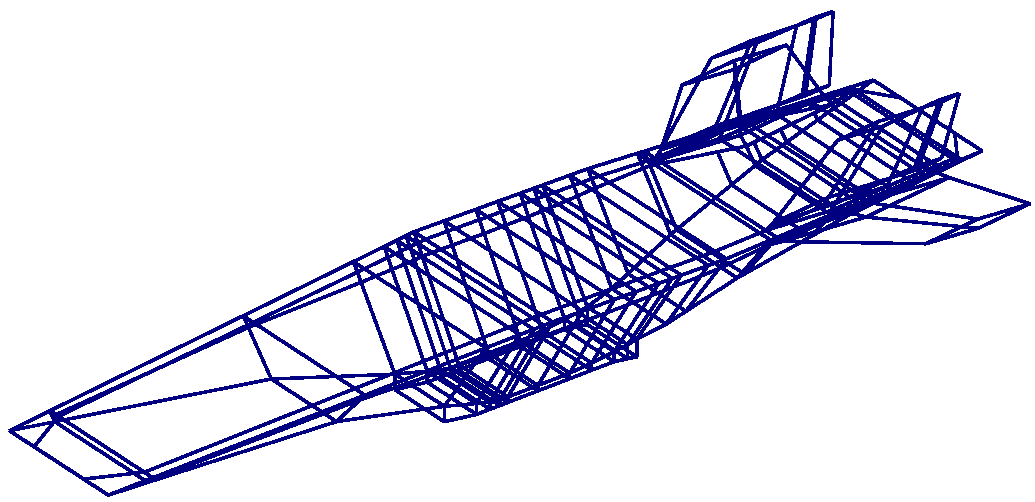
\includegraphics[width=4in]{./pics/frontispiece.pdf}}

% Default style for front pages
\frontpagestyle{1}

% Dedication
% \dedication{ %
% This dissertation is in honor of Adlai Stevenson and William Jennings
% Bryan, who were both twice the Democratic nominee for President of the
% United States without winning either time.  As an interesting side note,
% Adlai Stevenson's grandfather, Adlai E. Stevenson I, was William
% Jennings Bryan's running mate in the 1900 election.
%}

% Acknowledgments
% \acknowledgments[6]{ %
% It is imperative that I thank all of the authors of the dissertation
% template from the Department of Atmospheric, Oceanic and Space Sciences,
% which is available online at
% \href{http://aoss.engin.umich.edu/pages/current/dissertation-template}{%
% http://aoss.engin.umich.edu/}.  To my knowledge, the authors of that
% template include Jin Ji, Roque D. Oliveira, and Jason Gilbert.  I also
% must thank Sara Spangelo for suggesting that this template be ready by
% the end of April 2011.}
% This command sets the width of the acknowledgments area as a fraction
% of the total width of the text area.
\acknowledgmentswidth{0.8}

% Preface
% \preface[2]{ %
% The text of this document is of course mainly meant to show how the
% template works.  The topic is thus a basic problem which has been solved
% in a great number of ways.  This sample topic, which is solving
% equations of one variable using iterative techniques, allows us to use
% sample equations and figures so that we can see how they will look in
% this template.  In addition to this subject, the text also serves as a
% very unusual users' manual.  Chapter \ref{chap:manual}, which does not
% match the other chapters at all, gives instructions on the actual
% commands that are used with this template.}

% Committee
\committee{ %
Software Center, IAPCM, Beijing China}
%University of Michigan, Ann Arbor, USA (In honor of)

% Chair must be entered separately for formatting reasons.
% \chair{James F. Driscoll}

% Commands to hide or show lists of figures, tables, etc.
%\hidelistoftables
\showlistofprograms
\showlistofappendices

% Definition of any abbreviations used.
\abbreviations{
 \acro{CFD}{Computational Fluid Dynamics}
 \acro{MSRSF}{Monotonic, Single-Root Scalar Function}
}

% Some abstract text
\abstract{
The OpenJOY program is an open source nuclear data processing framework, which intends to provide the community a research tool that enables them to test new ways of development.}
%\hideabstractpagenumber

\usepackage{array}
\newcolumntype{L}[1]{>{\raggedright\let\newline\\\arraybackslash\hspace{0pt}}m{#1}}
\newcolumntype{C}[1]{>{\centering\let\newline\\\arraybackslash\hspace{0pt}}m{#1}}
\newcolumntype{R}[1]{>{\raggedleft\let\newline\\\arraybackslash\hspace{0pt}}m{#1}}
\usepackage[]{algorithm2e}
\usepackage{longtable}

%% DOCUMENT AREA
\begin{document}


\chapter{Introduction}   \label{chap:intro}

\chapter{CMS: Constants Maintenance System} \label{chap:cms}
We begin with the discussion of a very simple module of the OpenJOY: the constants maintanance system (CMS), which defines the commonly used constants across the computer codes.

\section{List of constants used}
The constants commonly used are listed in Table \ref{tb:cms_consts}.
\begin{table}[htb]
\centering
\caption{The constants commonly used in OpenJOY}
\begin{tabular}{L{2cm} | L{4cm} | L{6cm}}
\hline
Symbol & Meaning & Value \\\hline
$k$ & Boltzmann Constant & $8.6173324\times10^{-11}$ MeV/K, $8.6173324\times10^{-5}$ eV/K \\\hline
\end{tabular}
\label{tb:cms_consts}
\end{table}


\section{C++ Data Structures}
The data structure used in the computer code is given below.
\begin{program}[!htb]
\centering
\begin{verbatim} 
class CMS {
public:
    // Boltzmann Constants
    constexpr static const double BoltzmannMevK = 8.6173324e-11;
    constexpr static const double BoltzmannEvK  = 8.6173324e-5;
    
};
\end{verbatim}
\caption{ \label{program:ndls_cpp_api}
C++ public APIs for CMS module}
\end{program}

\chapter{NIST: NIST Nuclear Data System} \label{chap:nist}
\section{Isotopes and Elements}
The purpose of the NIST module is for describing all elements and isotopes in an organized format. The ENDF material identifier and ACE ZAID identifier number are mapped to a NIST element or isotope or even its excited meta state. This module serves as a base for linking evaluated nuclear files between different evaluation system. 

\begin{small}
\begin{longtable}{| l | c | c || l | c | c |}
\hline 
Isotopes & ENDF ID & ACE ZAID & Isotopes & ENDF ID & ACE ZAID \\ \hline
H-$n$ & $125+3(n-1)$ & $1000+n$ & He-$n$ & $225+3(n-3)$ & $2000+n$ \\ \hline
Li-$n$ & $325+3(n-6)$ & $3000+n$ & Be-$n$ & $425+3(n-9)$ & $4000+n$ \\ \hline
B-$n$ & $525+3(n-10)$ & $5000+n$ & C-$n$ & $625+3(n-12)$ & $6000+n$ \\ \hline
U-$n$ & $9225+3(n-234)$ & $92000+n$ & & & \\ \hline
H-1 & 125 & 1001 & & & \\ \hline
H-1 & 125 & 1001 & & & \\ \hline
H-1 & 125 & 1001 & & & \\ \hline
H-1 & 125 & 1001 & & & \\ \hline
H-1 & 125 & 1001 & & & \\ \hline
H-1 & 125 & 1001 & & & \\ \hline
H-1 & 125 & 1001 & & & \\ \hline
H-1 & 125 & 1001 & & & \\ \hline
H-1 & 125 & 1001 & & & \\ \hline
H-1 & 125 & 1001 & & & \\ \hline
H-1 & 125 & 1001 & & & \\ \hline
H-1 & 125 & 1001 & & & \\ \hline
H-1 & 125 & 1001 & & & \\ \hline
H-1 & 125 & 1001 & & & \\ \hline
H-1 & 125 & 1001 & & & \\ \hline
H-1 & 125 & 1001 & & & \\ \hline
H-1 & 125 & 1001 & & & \\ \hline
H-1 & 125 & 1001 & & & \\ \hline
H-1 & 125 & 1001 & & & \\ \hline
H-1 & 125 & 1001 & & & \\ \hline
H-1 & 125 & 1001 & & & \\ \hline
H-1 & 125 & 1001 & & & \\ \hline
H-1 & 125 & 1001 & & & \\ \hline
H-1 & 125 & 1001 & & & \\ \hline
H-1 & 125 & 1001 & & & \\ \hline
H-1 & 125 & 1001 & & & \\ \hline
\caption{Meaning for ENDF material id and ACE ZAID}
\label{tab:endf-ace-id-table}
\end{longtable}
\end{small}

\chapter{ENDF: ENDF Evaluated File System} \label{chap:endf}
\section{ENDF-6 Format}
The ENDF neutron data-files are stored in text files. Each row of the text file is an array of 80 characters. The first 66 characters are formatted depending on the type of the record. Then it follows by 4 characters of material number (MAT), 2 characters of file number (MF), 3 characters of section number (MT), and 5 characters of line number (NS). An illustration of the line structure is shown in Figure \ref{fig:endf-6-record}. The data array at the beginning contains 66 characters whose form depends on the type of the record.  The possibilities are:

\begin{itemize}
\item A string of 66 characters, or
\item Six numbers with each occupying 11 characters.
\end{itemize}

\begin{figure}[h]
\begin{center}
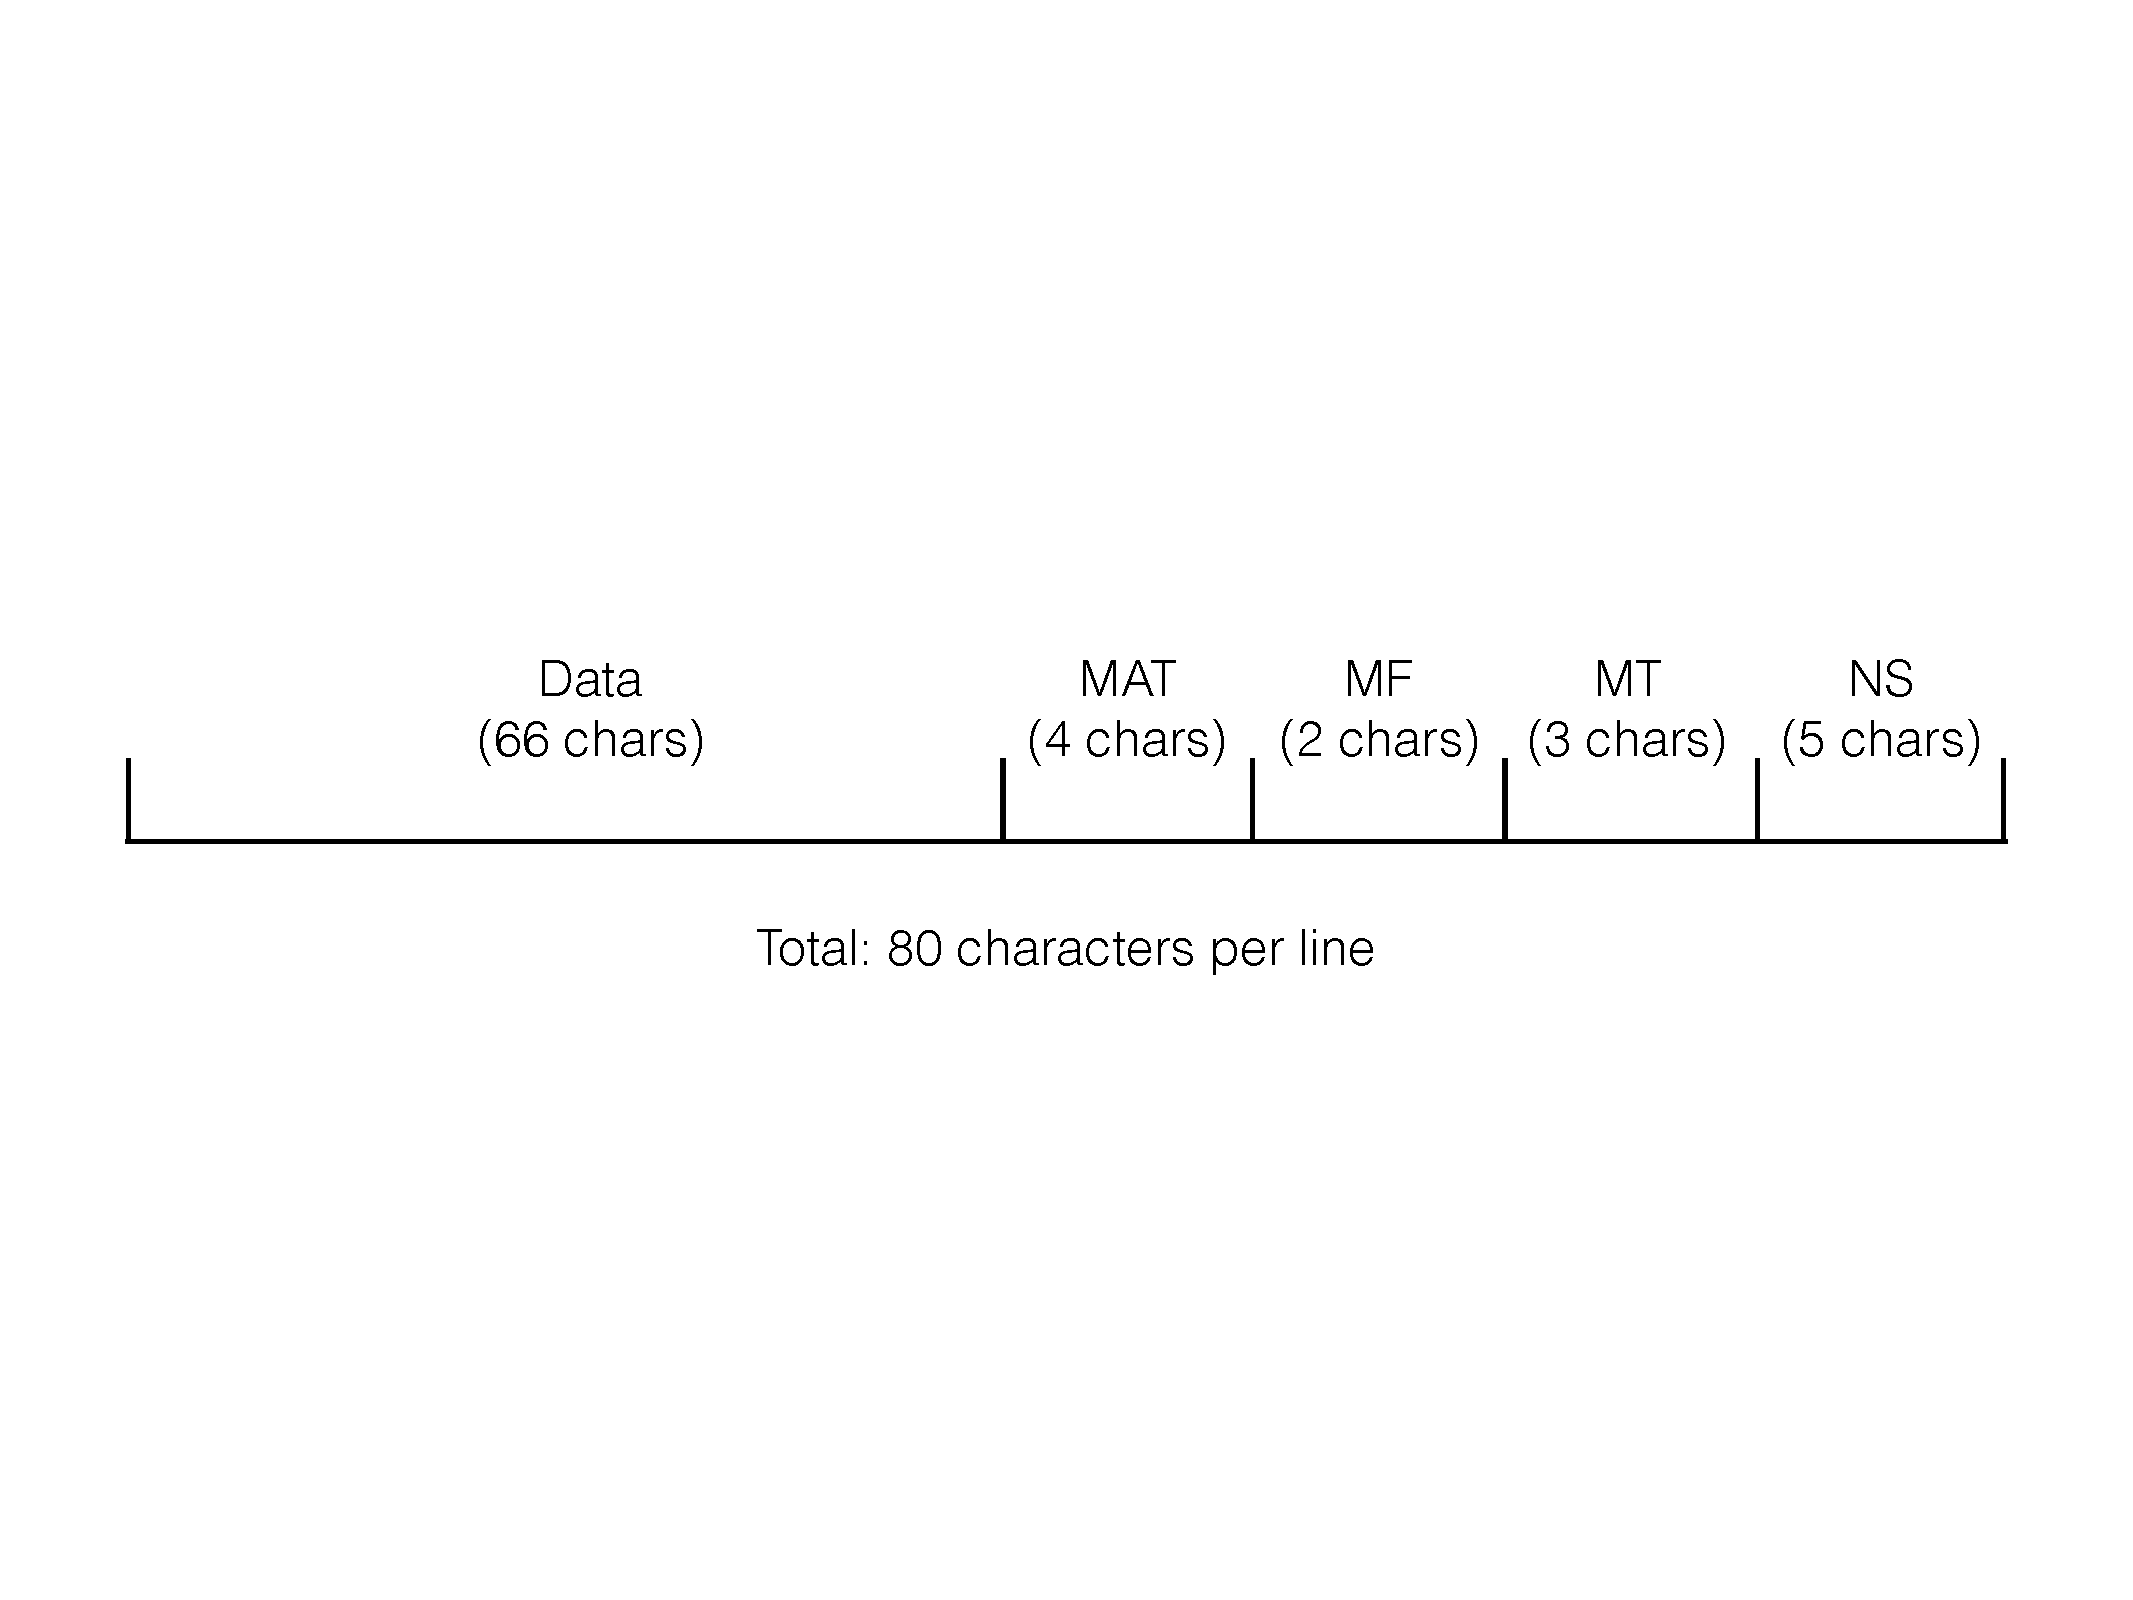
\includegraphics[scale=0.4]{./pics/endf-6-record.pdf}
\end{center}
\caption{ \label{fig:endf-6-record}
An example line of record for ENDF file}
\end{figure}

The ENDF-6 format specifies five types of commonly used records: TEXT, CONT, LIST, TAB1, and TAB2. 

\subsection{TEXT Records}
A TEXT records describes some text information, for example the meta information of the cross section.. The data section of the TEXT record is contains only one field: HL, which takes 66 characters. An illustration of the text record is shown in Figure \ref{fig:endf-6-record-text}.

\begin{figure}[h]
\begin{center}
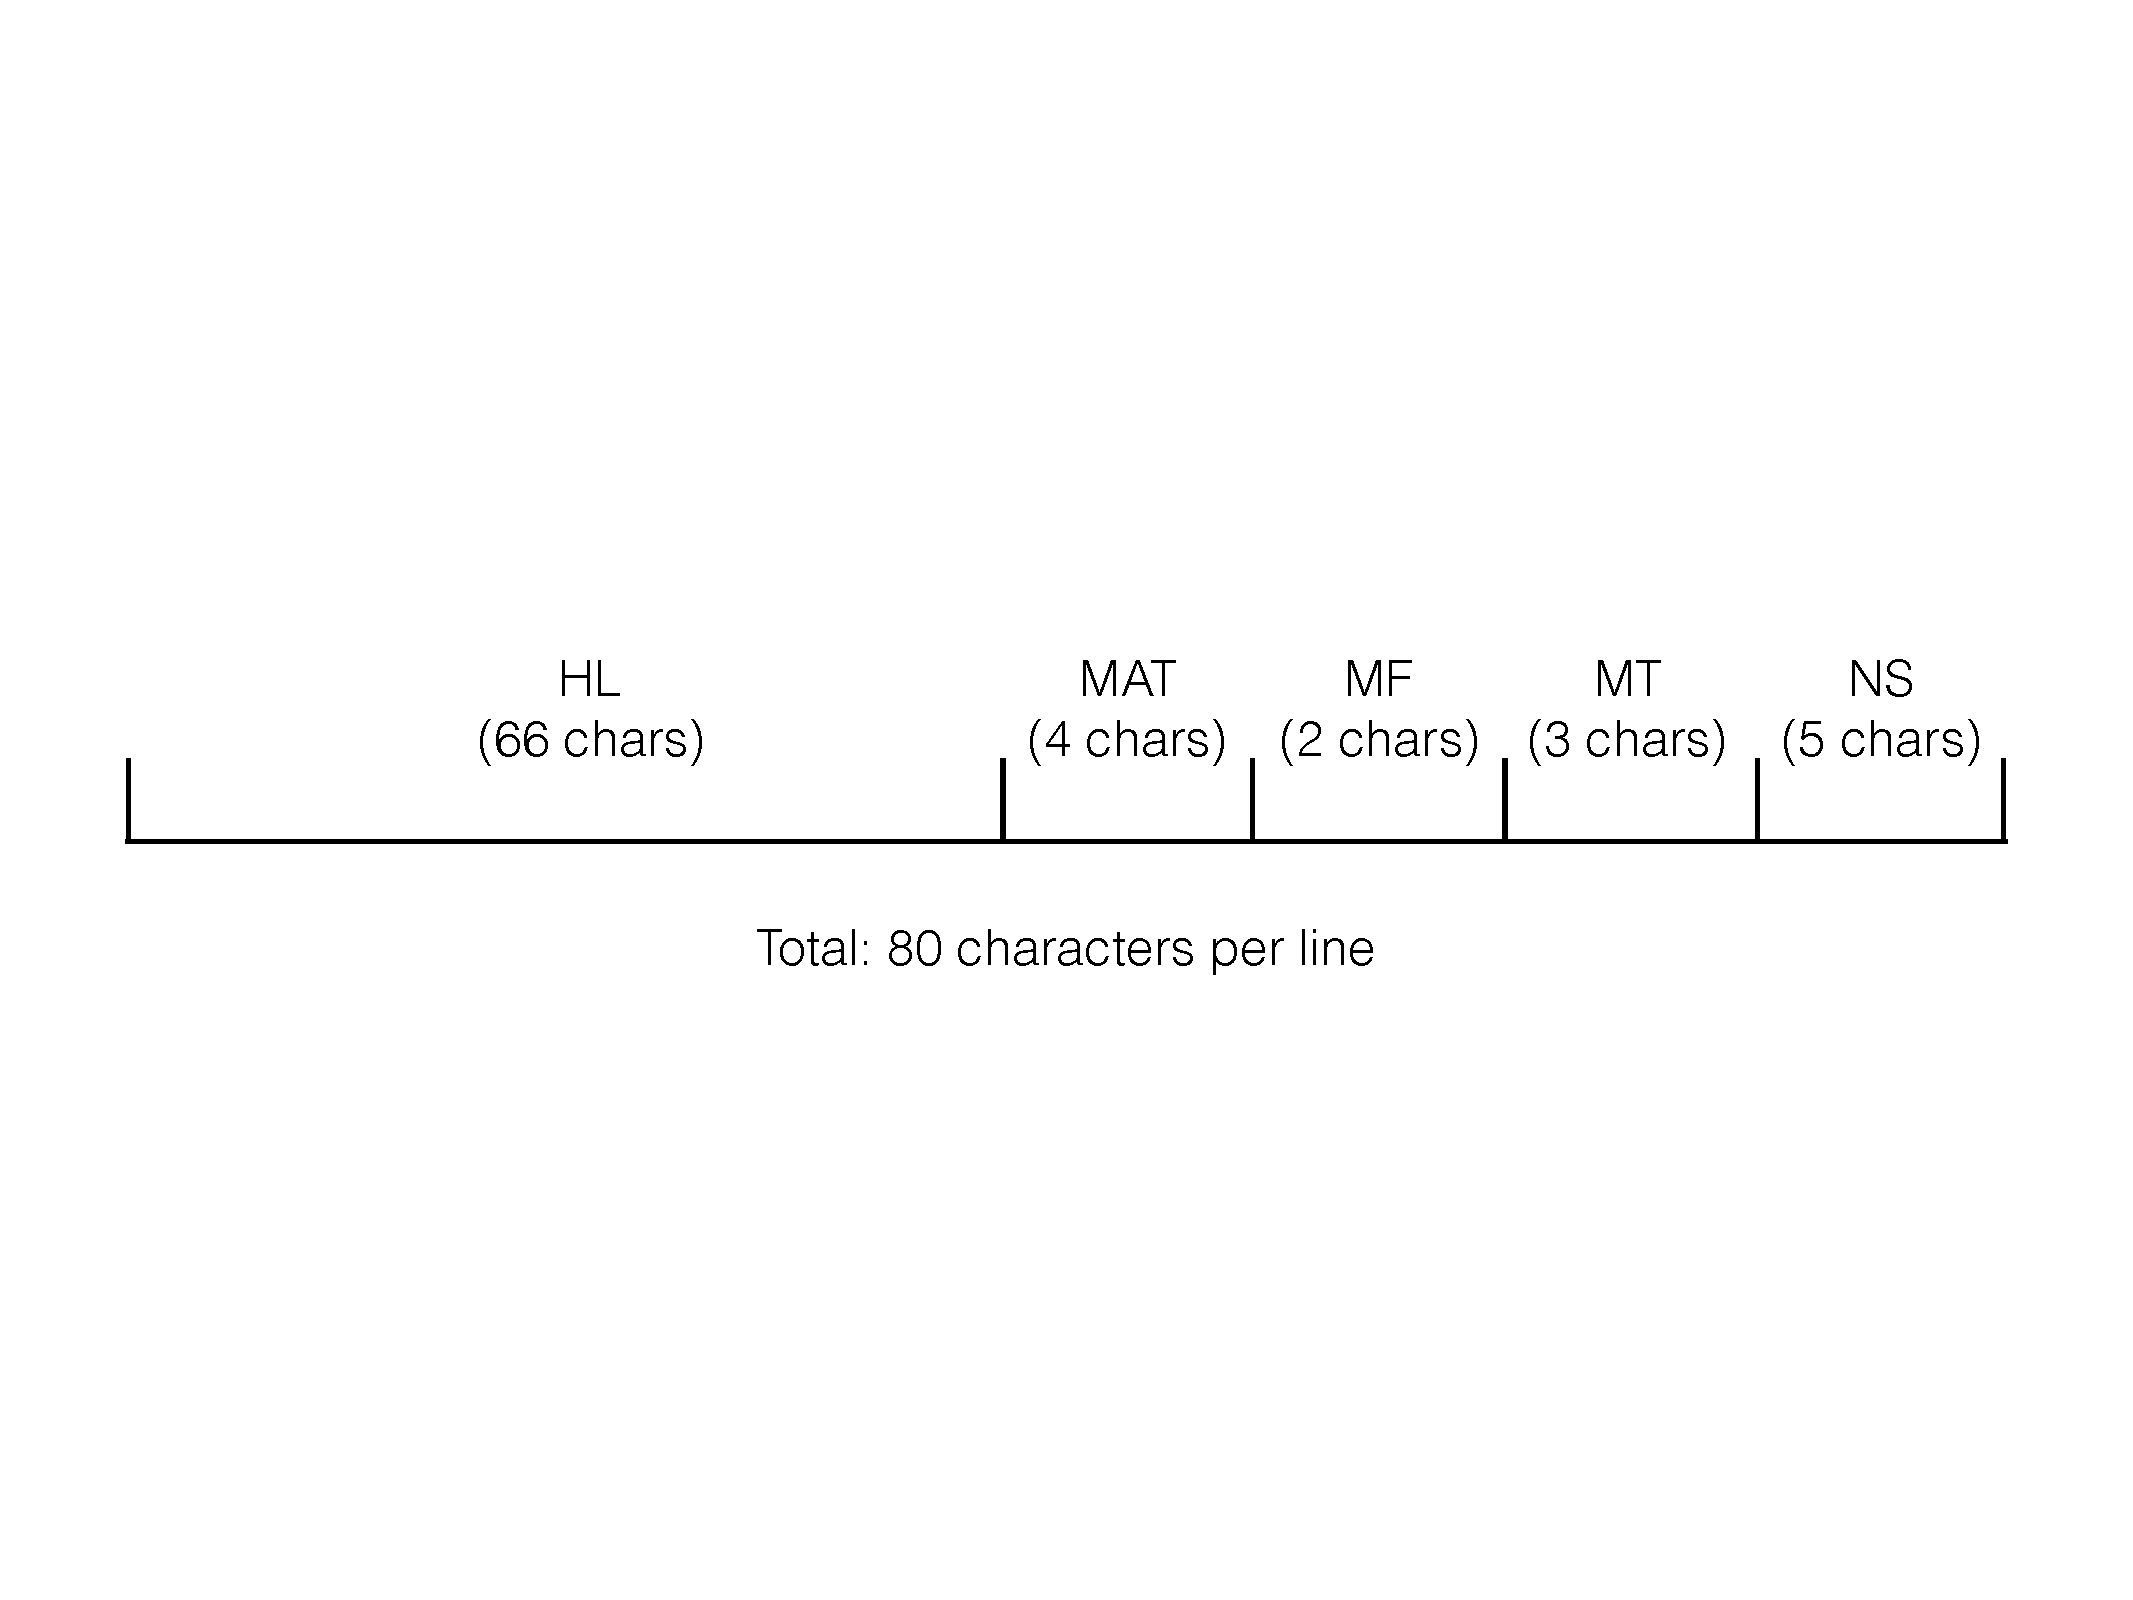
\includegraphics[scale=0.4]{./pics/endf-6-record-text.pdf}
\end{center}
\caption{ \label{fig:endf-6-record-text}
An example line of TEXT record for ENDF file}
\end{figure}

\subsection{CONT Records}
A CONT record includes some control information. The data field contains six floating numbers: C1, C2, L1, L2, N1 and N2. An illustration of the structure is shown in Figure \ref{fig:endf-6-record-cont}.

\begin{figure}[h]
\begin{center}
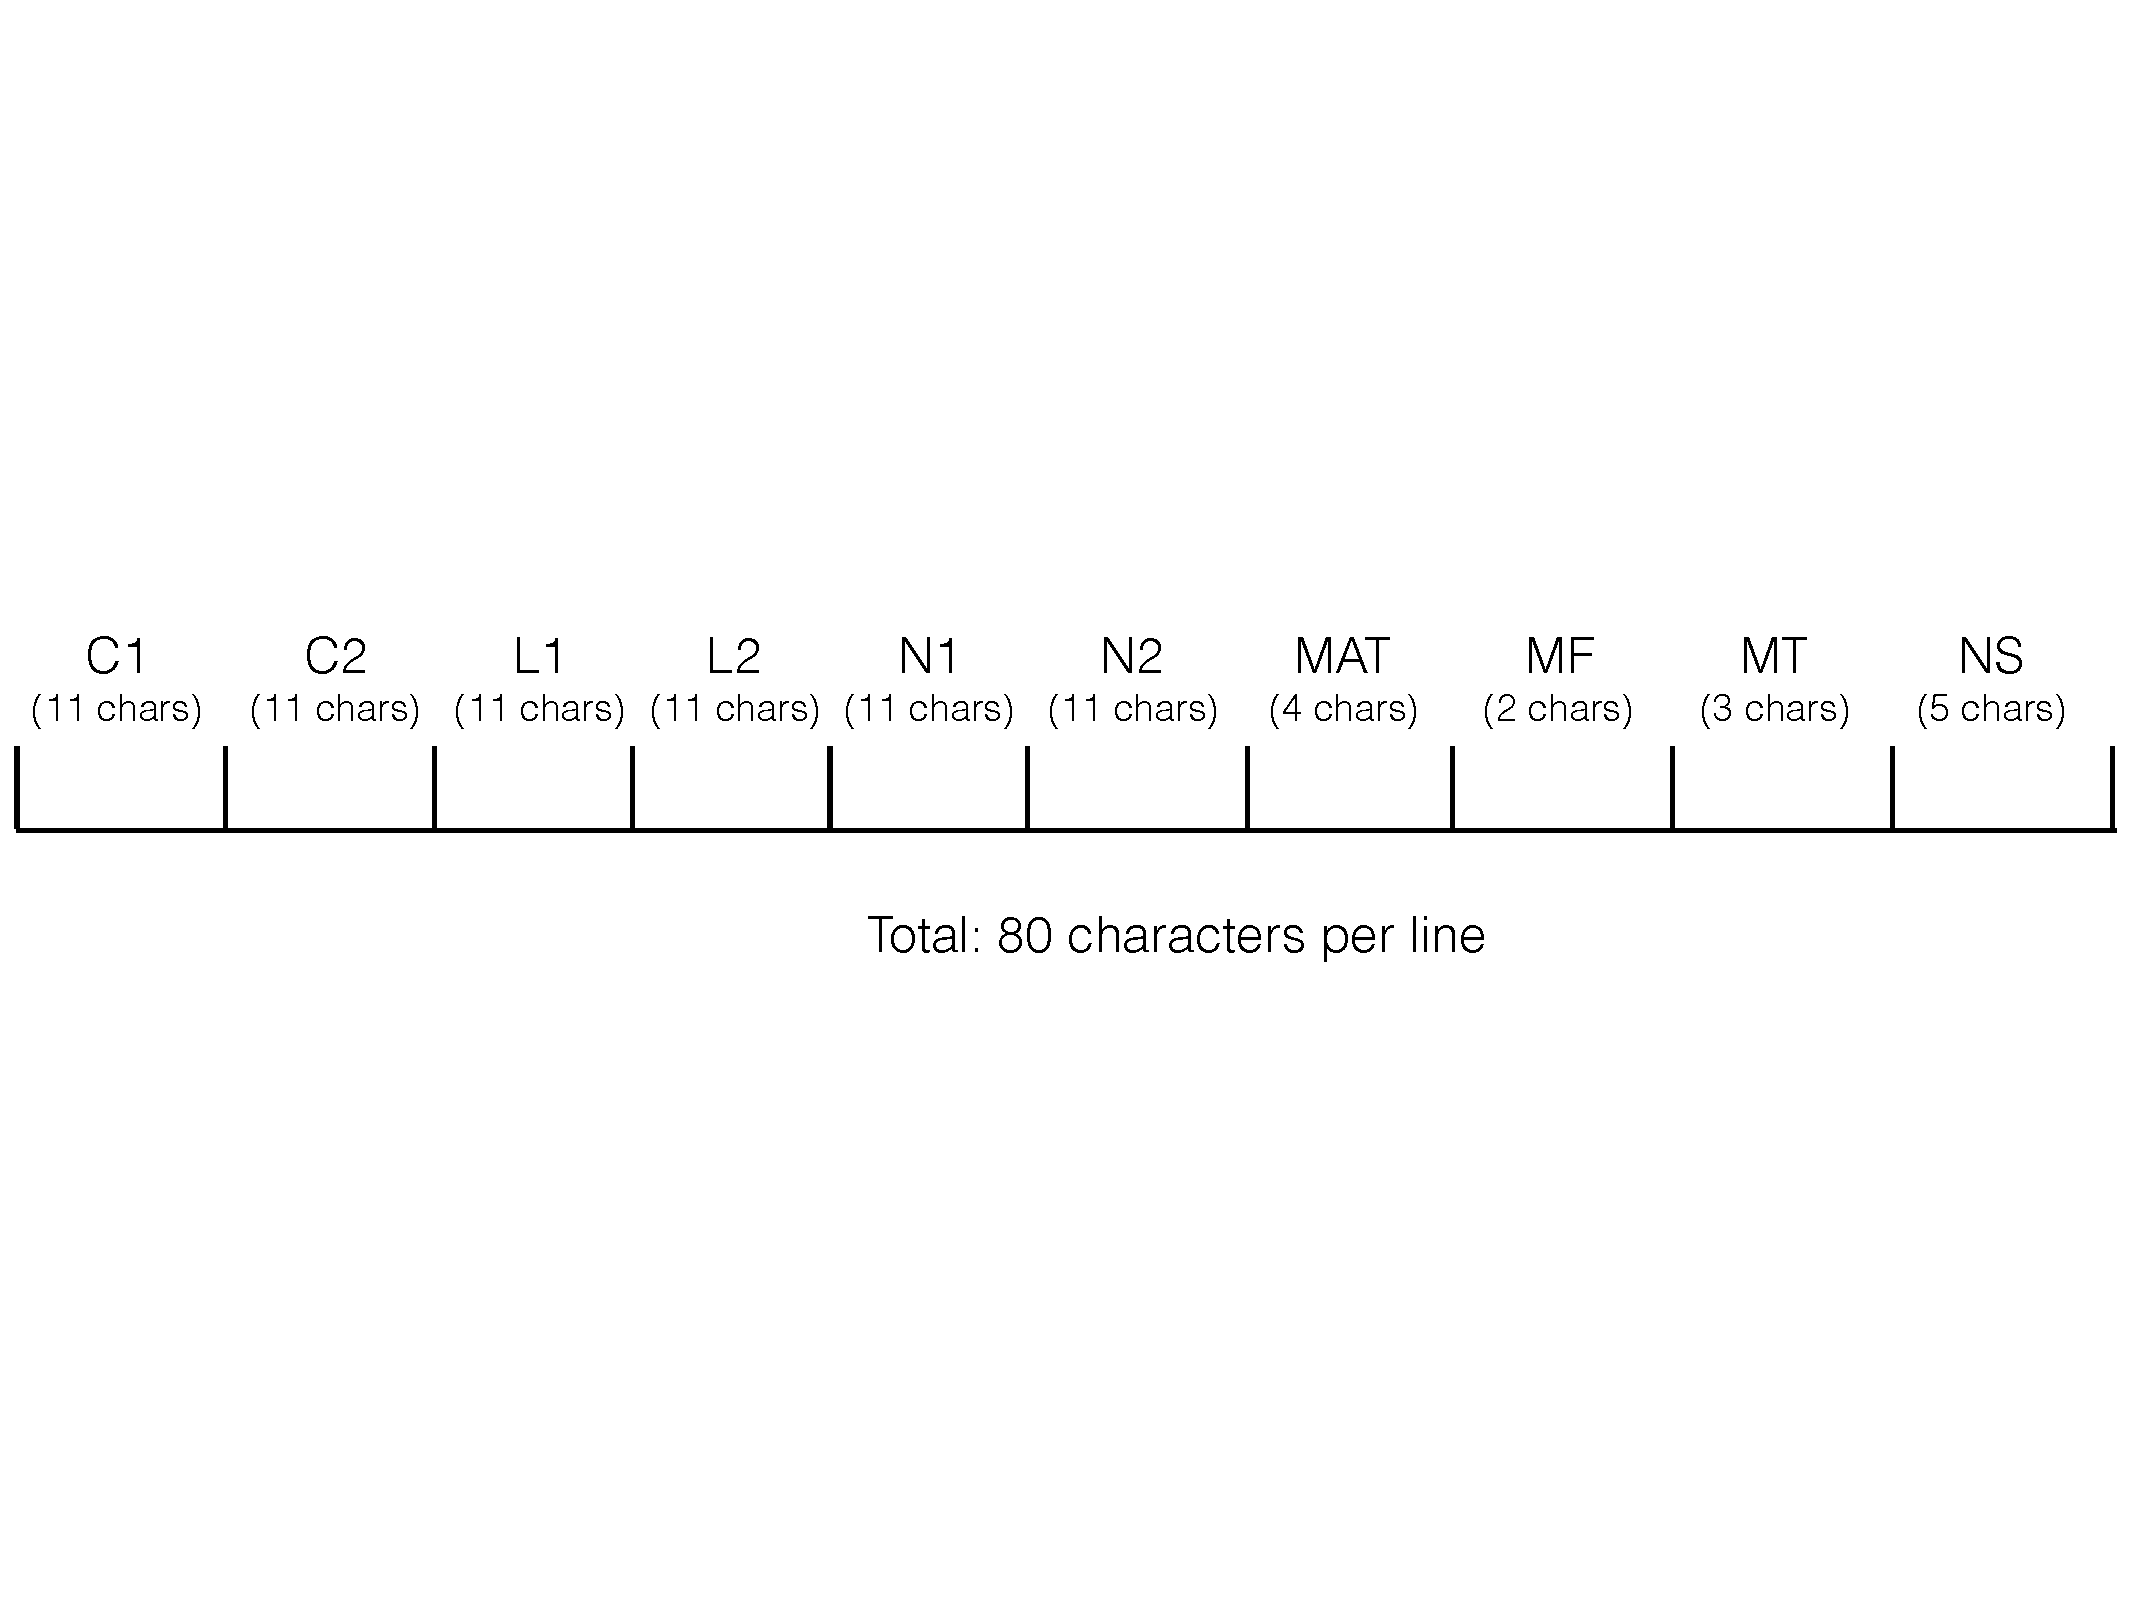
\includegraphics[scale=0.4]{./pics/endf-6-record-cont.pdf}
\end{center}
\caption{ \label{fig:endf-6-record-cont}
An example line of CONT record for ENDF file}
\end{figure}

\subsection{LIST Records}
A LIST record encodes a list of numbers. The records contains multiple lines, where the first line is a CONT record, and followed by a list of numbers organized into packages of 6 numbers. An illustration of these lines are shown in Figure \ref{fig:endf-6-record-list}. The length of list is stored in the 5th argument in the variable NPL in the first line. NPL needs not to be a multiple of 6, since the empty spaces in the list will be filled up with zeros.

\begin{figure}[h]
\begin{center}
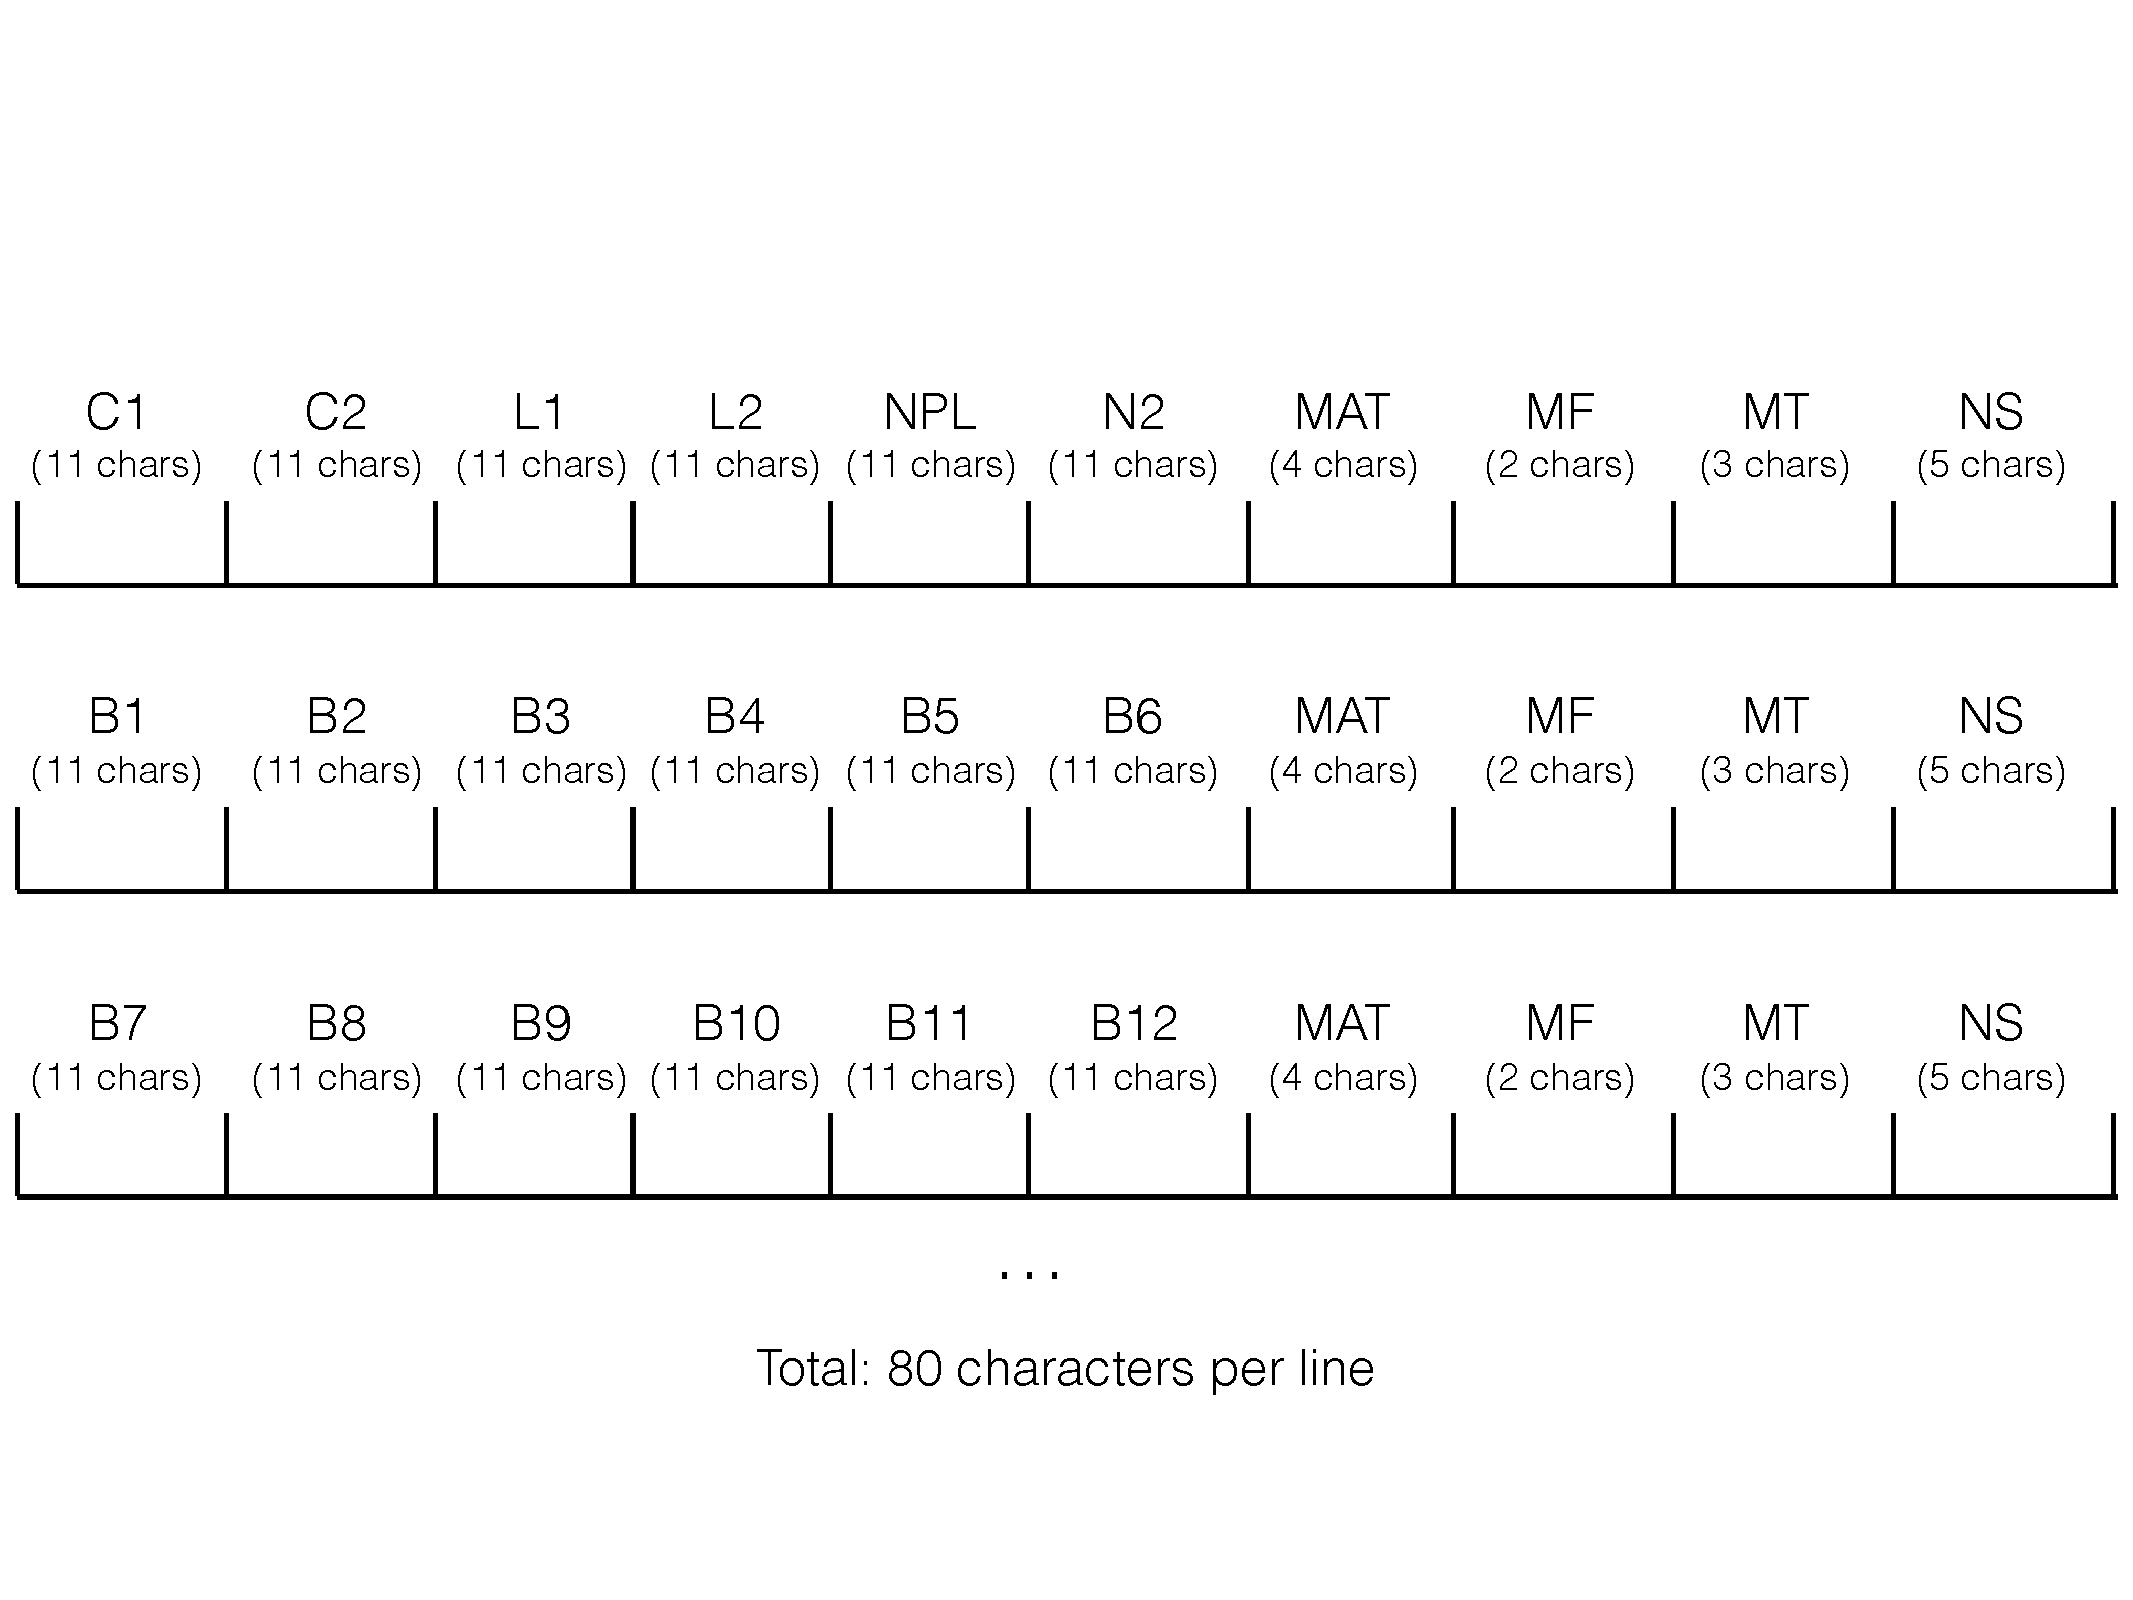
\includegraphics[scale=0.4]{./pics/endf-6-record-list.pdf}
\end{center}
\caption{ \label{fig:endf-6-record-list}
An example line of LIST record for ENDF file}
\end{figure}

\subsection{TAB1 Records}
A TAB1 record contains a one-dimensional tabulated functions such as $y(x)$. To describe the table function, four lists of data are presenting: NBT, INT, X, and Y. The dimensions of NBT and INT are NR, and the dimensions of X and Y are NP. This section of data contains a control record at the beginning, then followed by pairs of (NBT, INT) and pairs of (X, Y). An illustration of the storage format is shown in Figure \ref{fig:endf-6-record-tab1}.

\begin{figure}[h]
\begin{center}
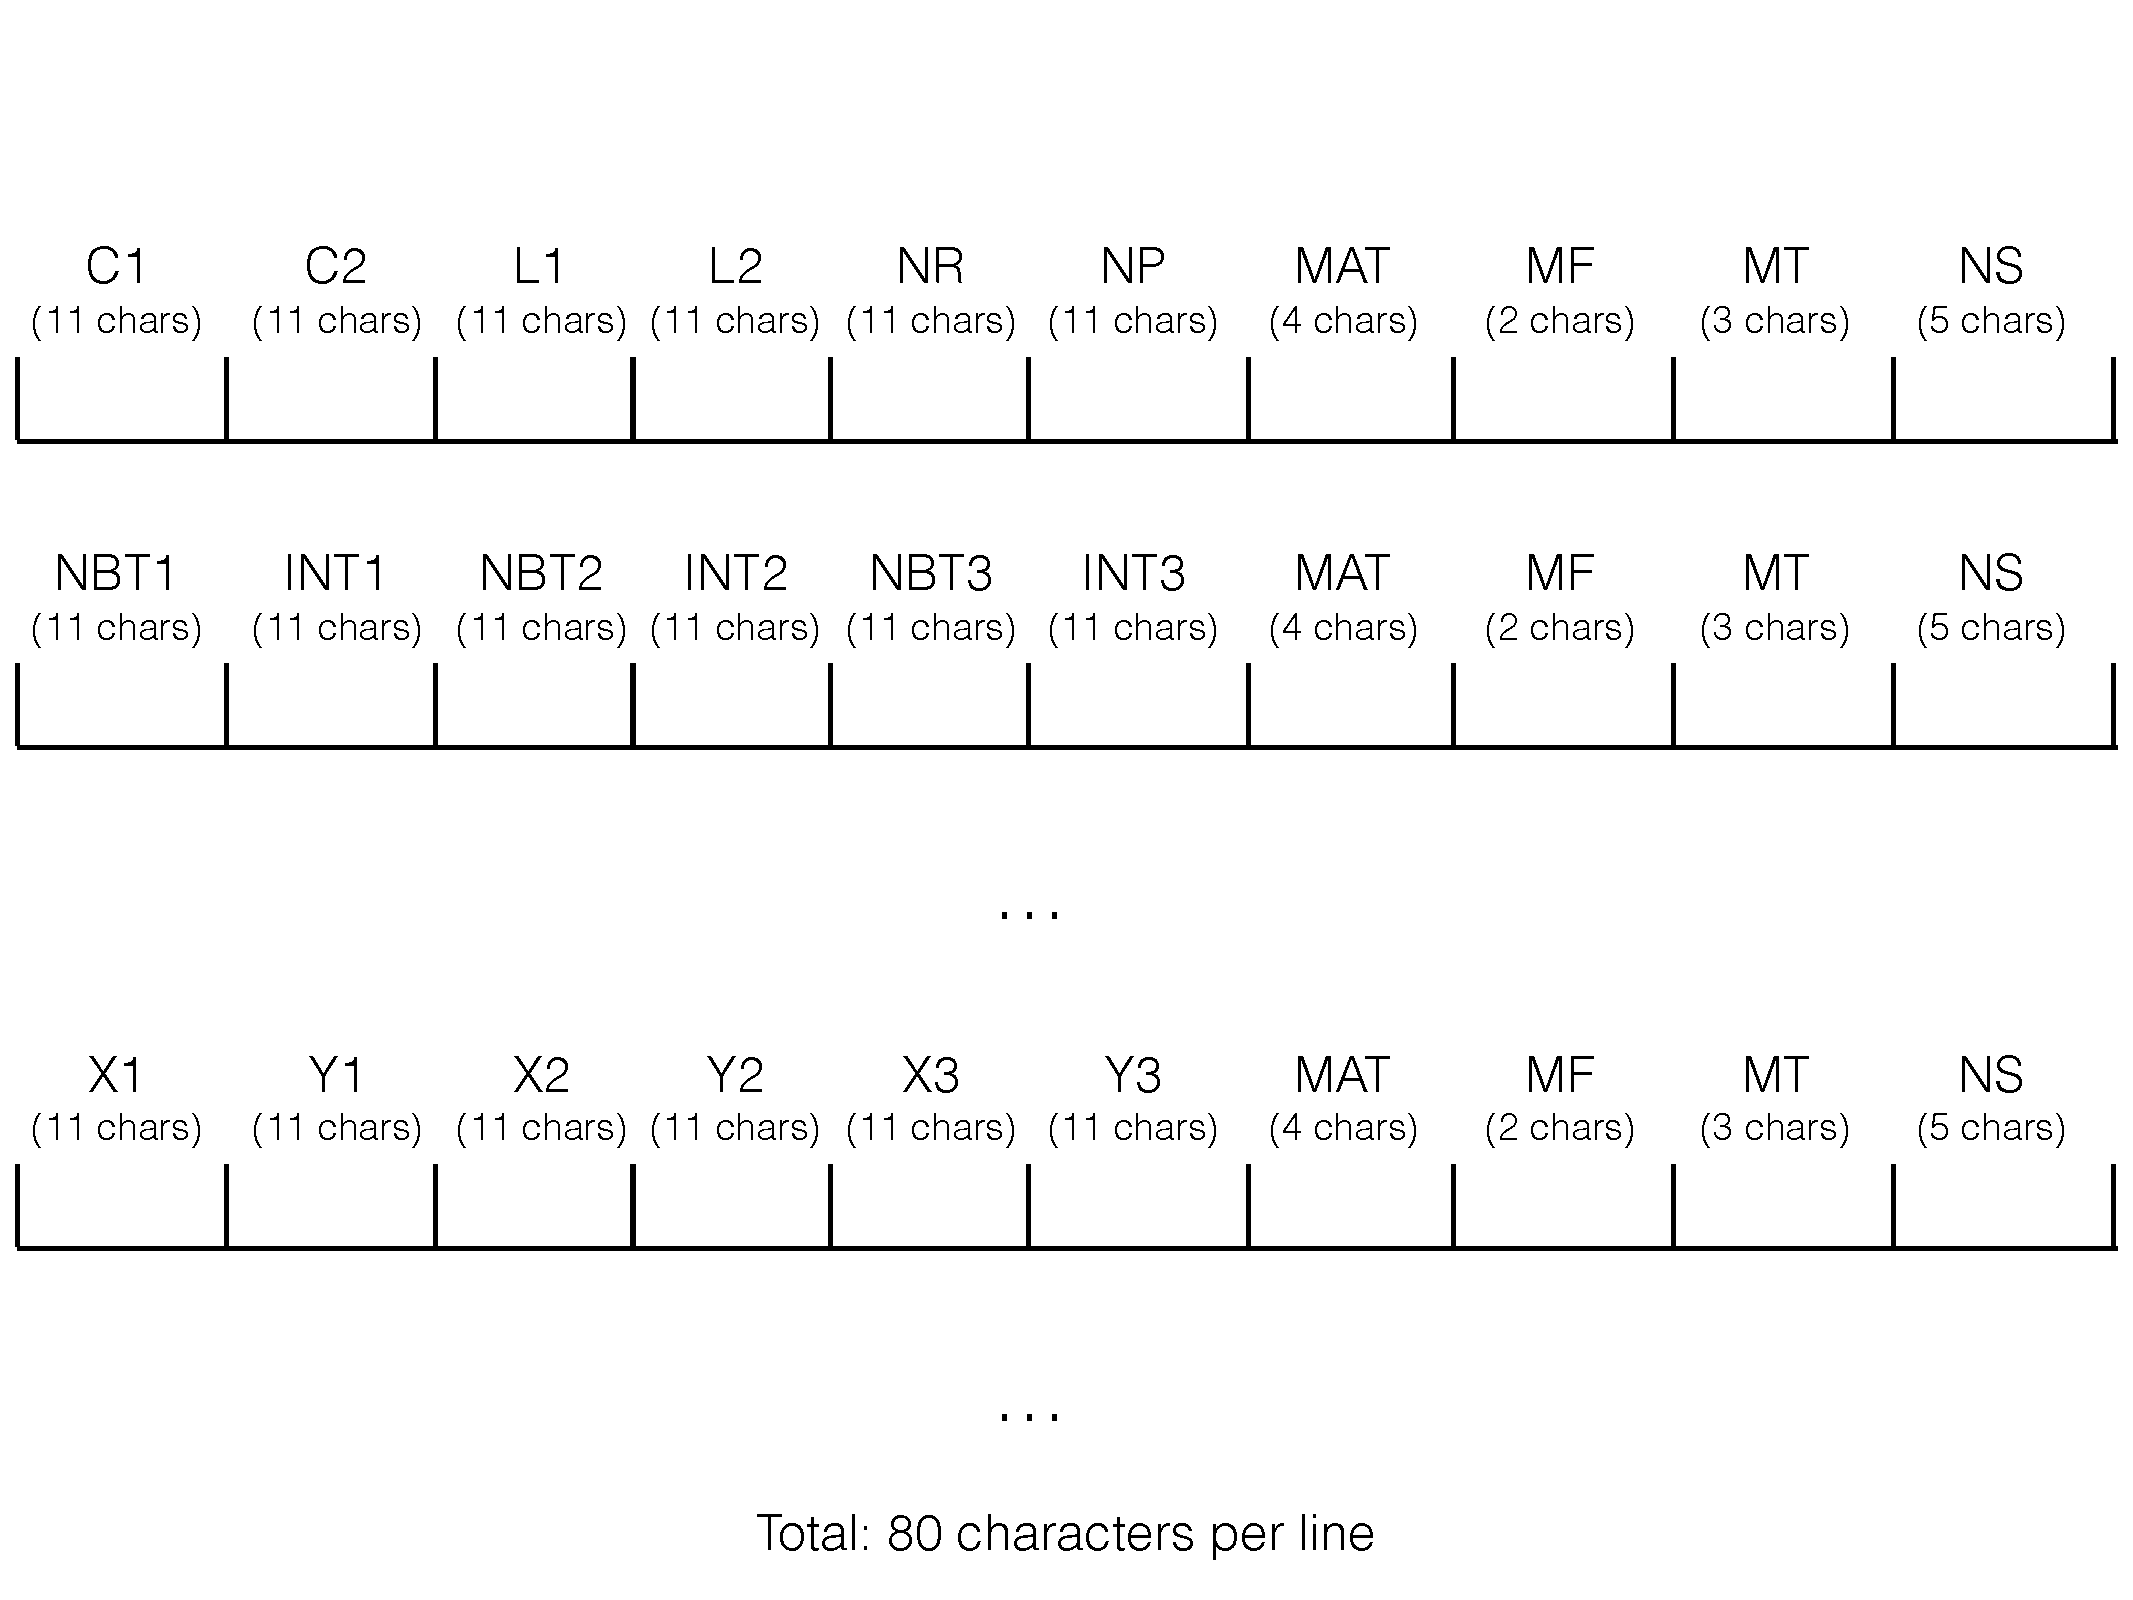
\includegraphics[scale=0.4]{./pics/endf-6-record-tab1.pdf}
\end{center}
\caption{ \label{fig:endf-6-record-tab1}
An example line of TAB1 record for ENDF file}
\end{figure}

\subsection{TAB2 Records}
A TAB2 record contains a two-dimensional tabular functions such as $y(x,z)$. The TAB2 records storages a list of data points for the $z$ variable and the interpolation rules in the NBT and INT array. It follows by NZ records with the C2 designated for the corresponding $z$ value. The possible records followed are either TAB1 or LIST record. An illustration of the format of storage is shown in Figure \ref{fig:endf-6-record-tab2}.

\begin{figure}[h]
\begin{center}
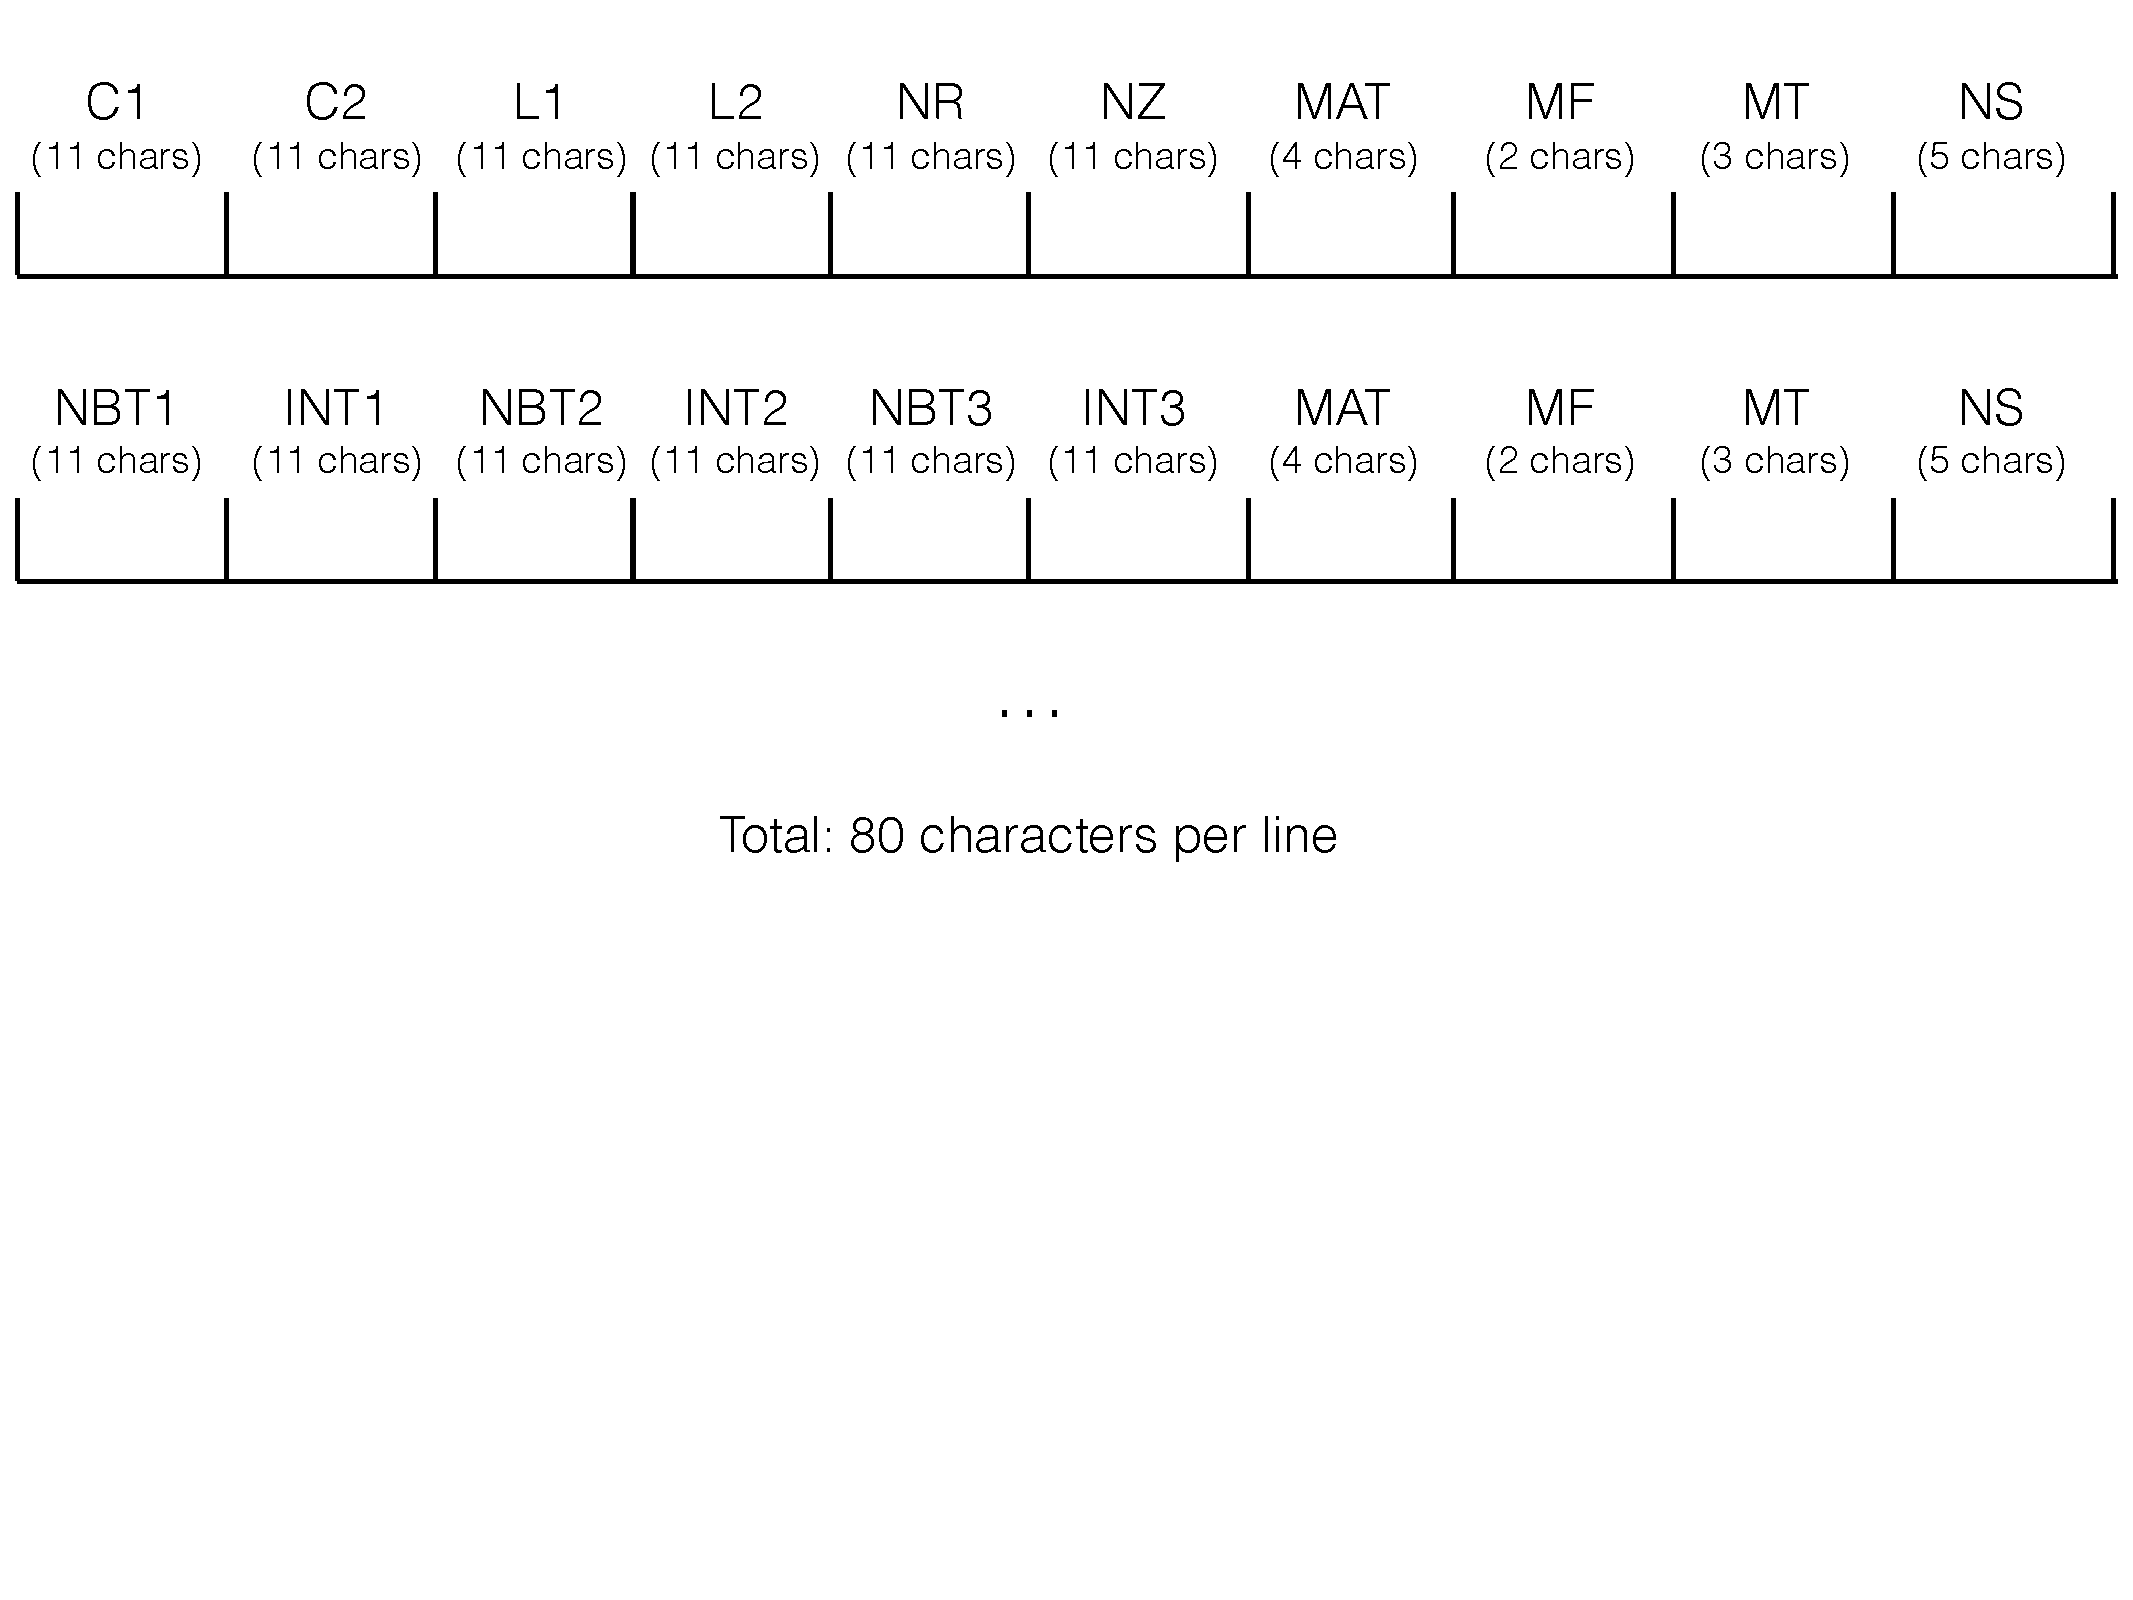
\includegraphics[scale=0.4]{./pics/endf-6-record-tab2.pdf}
\end{center}
\caption{ \label{fig:endf-6-record-tab2}
An example line of TAB2 record for ENDF file}
\end{figure}

\clearpage
\section{C++ Data Structure \& Application Interfaces}
The program is implemented native in C++ programming language, so in this section, we discuss the data structures first then the application interfaces.

The top level neutron data structure contains several major parts: the fission yield data, the reaction data, and the resonance data, as followed. 
\begin{verbatim} 
struct ENDFNeutronData {

    ... definitions of support data structures ...

    /* Key data structures for neutron data */
    
    // The fission yield information, from File 1 and 5
    YieldData                  fissionYield;
    
    // List of reactions information, from File 3
    std::vector<ReactionData>  reactions;
    
    // List of resonances information, from File 2
    std::vector<ResonanceData> resonances;
}
\end{verbatim}
The discussion begins with lower level data structures, and then discuss each major part in details.

\subsection{Fundamental Computational Data Structures}

\begin{itemize}
\item{\em Interpolation function: } 
The law of interpolation is a structure contains two fields: INT for the interpolation form, and NBT for the interpolation index.
\begin{verbatim} 
struct ENDFInterpLaw {
    long INT = -1;
    long NBT = -1;
};
\end{verbatim}
The law of interpolation is used in a list, i.e. 
\begin{verbatim} 
std::vector<ENDFInterpLaw> 
\end{verbatim}
, which is usually combined with a list of scattered function values with $x-y$ pairs. One such pair is called a datapoint, which is defined in a structure as followed:
\begin{verbatim} 
template <typename T>
struct ENDFObjectDataPoint {
    double x = 0.;
    T y;
};
\end{verbatim}
$x$ value is a scalar of floating number, and the $y$ value can be any object, and is expressed in a C++ template class parameter. A special case where $y$ is a scalar floating number as well is defined as a special type ENDFDataPoint.
\begin{verbatim} 
typedef ENDFObjectDataPoint<double>   ENDFDataPoint;
\end{verbatim}
A tabular function is represented by a list of ENDFInterpLaw and a list of ENDFDataPoint:
\begin{verbatim}
struct ENDFInterpolationFunction {
    std::vector< ENDFInterpLaw > interp;
    std::vector< ENDFDataPoint > data;
    
    // Evaluate the interpolation function at point x
    double evaluate(double x) const;
};
\end{verbatim}
The meaning of the integer INT is listed in table \ref{tab:interp}.
\begin{table}[h]
\centering
\caption{Definition of interpolation laws}
\vspace{1ex}
\begin{tabular}{L{2cm} L{6cm}}
\hline 
INT & Interpolation Scheme \\
\hline
1 & $y$ is constant in $x$ \\
2 & $y$ is linear in $x$\\
3 & $y$ is linear in $\ln(x)$ \\
4 & $\ln(y)$ is linear in $x$ \\
5 & $\ln(y)$ is linear in $\ln(x)$\\
\hline
\end{tabular}
\label{tab:interp}
\end{table}
Next, we illustrate how to interpolate the function at any given $x$ with an example, as shown in Figure \ref{fig:endf-int-laws}, taken from the ENDF manual. In this function, we have 10 data points which splits into 3 regions, the NBT numbers are marked to indicate the upper boundaries of the regions. The INT numbers indicate the interpolation laws of the regions, as explained in Table \ref{tab:interp}. It is possible that two points share the same $x$-coordinate, and this point relates to a `jump' in the function. For a given $x$ between two points $(x_l, y_l)$ and $(x_r, y_r)$ with an interpolation law INT. Then, the interpolated $y$ is calculated by:
\begin{eqnarray}
y &=& y_l, \mbox{ if INT} = 1,\\[1ex]
y &=& y_l + \frac{x-x_l}{x_r-x_l}(y_r-y_l),  \mbox{ if INT} = 2,\\[1ex]
y &=& y_l + \frac{\log(x/x_l)}{\log(x_r/x_l)}(y_r-y_l),  \mbox{ if INT} = 3,\\[1ex]
y &=& y_l \left(\frac{y_r}{y_l}\right)^{\left(\frac{x-x_l}{x_r-x_l}\right)},  \mbox{ if INT} = 4,\\[1ex]
y &=& y_l \left(\frac{y_r}{y_l}\right)^{\left(\frac{\log(x/x_l)}{\log(x_r/x_l)}\right)},  \mbox{ if INT} = 5.
\end{eqnarray}

\begin{figure}[h]
\begin{center}
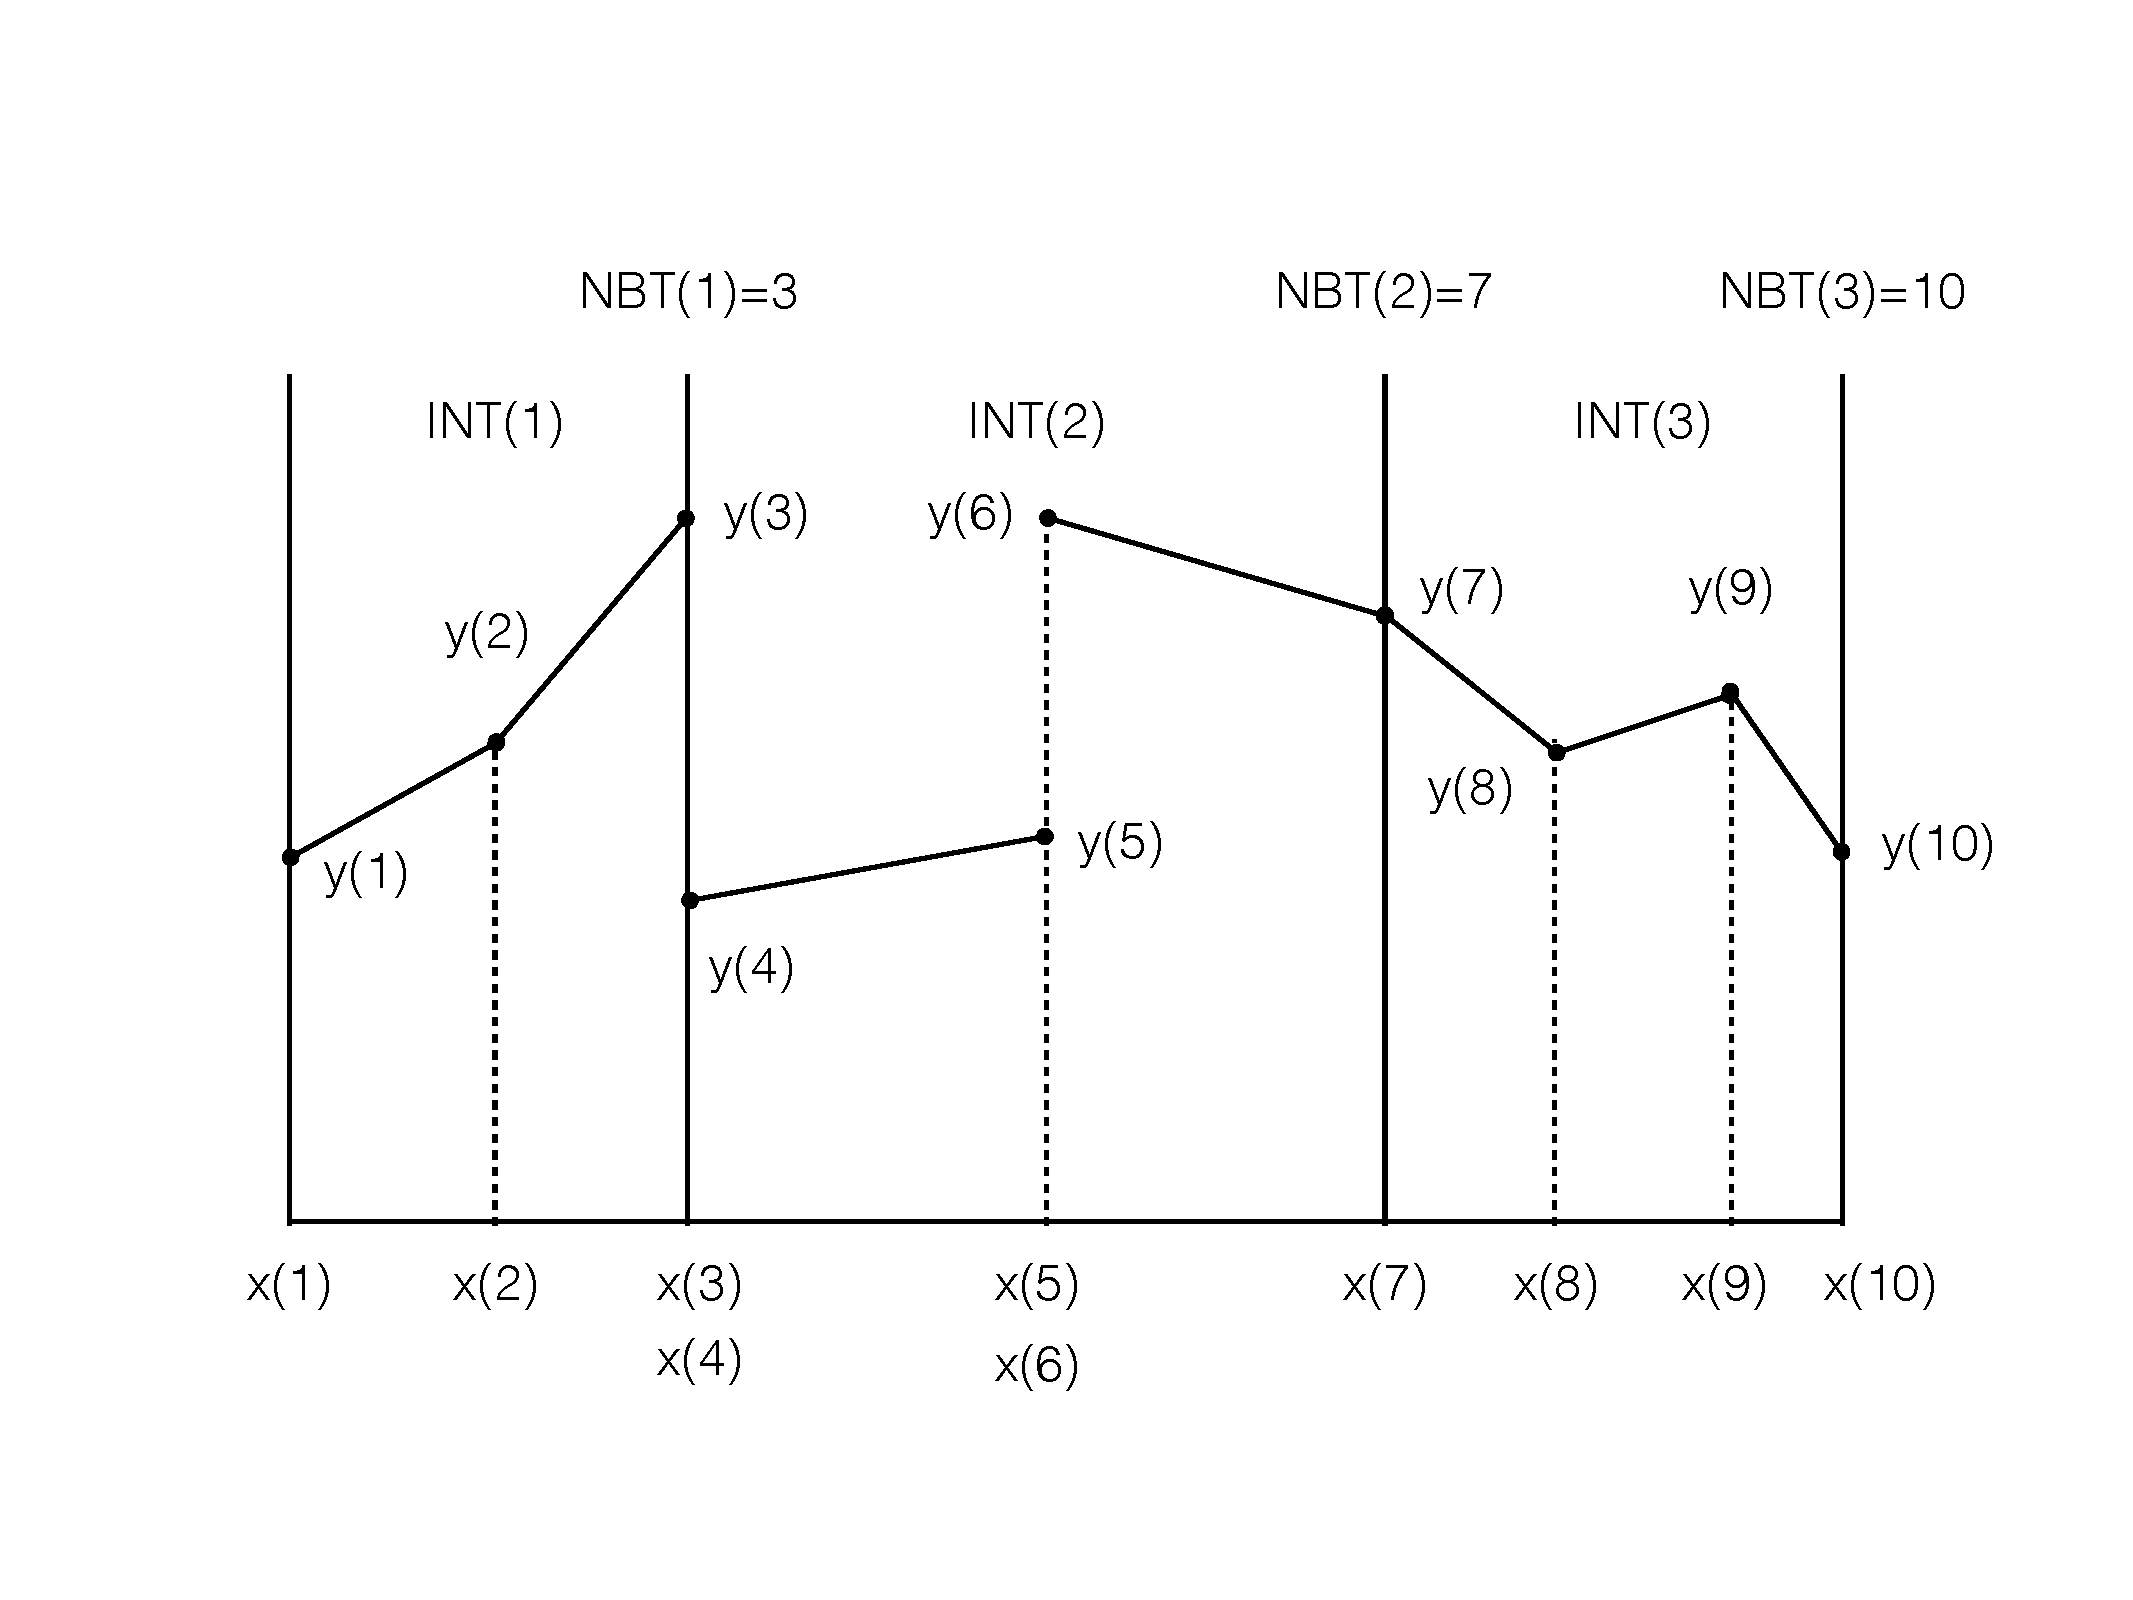
\includegraphics[scale=0.4]{./pics/endf-int-laws.pdf}
\end{center}
\caption{ \label{fig:endf-int-laws}
An example showing the ENDF interpolation rules of a function, the indices start from 1, but in C++ language, the indices start from 0}
\end{figure}
In the data structure, we have an public function`double evaluate(double x) const', which takes a given value $x$, and use the formula above to calculate the interpolated $y$.\\

\item{\em Polynomial function: } 
In the ENDF database, a function can be described by a polynomial with degree $n-1$ and coefficients $c_0, c_1, \dots, c_{n}$. The function value is evaluated by:
\begin{eqnarray}
y &=& \sum_{i=0}^{n-1}c_{i}\,x^i
\end{eqnarray}
The data structure for describing a polynomial function is given below:
\begin{verbatim}
struct ENDFPolynomialFunction {
    std::vector<double> coefficents;
    
    // Evaluate the polynomial function value at x
    double evaluate(double x) const;
};
\end{verbatim}
The `evaluate' function implements the evaluation of the function value at x.

\item{\em Function type: }
To specify whether a function is an ENDF interpolation or a polynomial, an enumeration is introduced as followed.
\begin{verbatim}
enum class ENDFFunctionType {
    INTERPOLATION = 1,
    POLYNOMIAL = 2
};
\end{verbatim}

\end{itemize}

\subsection{Fission Yield Data Structures}

The fission yield is an important property of the neutron data. For a fission nuclide, a fission can be prompt or delayed. Here, it discusses the data structures to describe the fission yield.

\begin{itemize}

\item{\em Fission spectrum: }
The fission spectrum describes the average number of neutron released as a function of the incident neutron energy. Such a function is denoted in $\bar{\nu}(E)$. For prompt fission, it is described as $\bar{\nu}_p(E)$, and for delayed fission, the sum is described as $\bar{\nu}_d(E)$. If there are $N$ precursor groups, the average number of neutron released from group $i$ is denoted as $\bar{\nu}_i(E)$, and
\begin{eqnarray}
\bar{\nu}_d(E) &=& \sum_{i=1}^{N}\bar{\nu}_i(E).
\end{eqnarray}
The average total fission neutron yield is given by $\bar{\nu}(E)$ and 
\begin{eqnarray}
\bar{\nu}(E) &=& \bar{\nu}_p(E) + \bar{\nu}_d(E).
\end{eqnarray}
The fission spectrum can be described either as an ENDF interpolation function or a polynomial function. So the data structure is listed as followed.
\begin{verbatim}
struct Spectrum {
    // The function type
    ENDFFunctionType type;
    // The data for interpolation function
    ENDFInterpolationFunction interpFunc;
    // The data for polynomial function
    ENDFPolynomialFunction polyFunc;
};
\end{verbatim}

\item{\em Precursor group: }
For precursor group $i$, there are the decay constant $\lambda_i$ and the group abundance $\alpha_i$. They can be either constant or energy dependent. So the precursors are described in the data structure as followed.
\begin{verbatim}
struct Precursor {
    // Decay constant, lambda
    double decayConst = 0.;
    // Decayed-group abundance, alpha
    double groupAbundance = 0.;
};
struct Precursors {
    // List of precursors
    std::vector<Precursor> precursors;
};
\end{verbatim}

\item{\em Neutron yield data: }
The neutron yield data is packed into a single data structure. The fission spectra are given in a C++ pointer. When the pointer is nullptr, then no such fission data is provided.
\begin{verbatim}
struct YieldData {
    ~YieldData();
    
    // Total neutron yield function
    Spectrum *total = nullptr;
    // Prompt neutron yield function
    Spectrum *prompt = nullptr;
    // Delayed neutron yield function
    Spectrum *delayed = nullptr;
    
    // Whether precursor is energy dependent
    bool isPrecursorEnergyDependent = false;
    // Energy independent precursors
    Precursors energyIndependentPrecursors;
    // Energy dependent precursors
    ENDFObjectInterpolationFunction< Precursors >
    energyDependentPrecursors;
};
\end{verbatim}

\end{itemize}

\subsection{Resonance Data Structure}

\begin{itemize}
\item
\end{itemize}

\subsection{Reaction Data Structure}
The reaction data structures taken from ENDF file 3 describe the `background' cross sections of reactions, which does not depend on the energy of the incident neutrons. The type of the reaction is determined by its `MT' number, whose definitions can be found in Table \ref{tab:mt-meaning}. The reaction cross sections are represented by the ENDF table with an `ENDFInterpolationFunction' data structure.
\begin{verbatim}
struct ReactionData {
    // Reaction number
    long   MT = -1;
    // Mass-difference Q value
    double QM = 0.;
    // Reaction Q value from the lowest energy state
    double QI = 0.;
    // Complex or "breakup" reaction flag
    long   LR = -1;
    // ENDF interpolated function for cross sections
    ENDFInterpolationFunction xsec;
};
\end{verbatim}

\begin{small}
\centering
\begin{longtable}{l l p{3.5cm} | l l p{3.5cm}}
MT & Symbol & Meaning & MT & Symbol & Meaning\\\hline
1 & (n,total) & total & 2 & (n,elastic) & elastic scattering\\\hline
3 & (n,inelastic) & inelastic scattering & 4 & (n,level) & level scattering\\\hline
5 & (n,other) & others & 11 & (n,2nd) & two neutrons plus one deuteron\\\hline 
16 & (n,2n) & two neutrons & 17 & (n,3n) & three neutrons\\\hline
18 & (n,fission) & fission & 19 & (n,f) & f \\\hline
20 & (n,nf) & one neutron and f & 21 & (n,2nf) & two neutrons and f\\\hline
22 & (n,na) & one neutron and one alpha & 23 & (n,n3a) & one neutron and three alphas\\\hline
24 & (n,2na) & two neutrons and one alpha & 25 & (n,3na) & three neutrons and one alpha\\\hline
28 & (n,np) & one neutron and one proton & 29 & (n,n2a) & one neutron and two alphas\\\hline
30 & (n,2n2a) & two neutrons and two alphas & 32 & (n,nd) & one neutron and one deuteron\\\hline
33 & (n,nt) & one neutron and one triton & 34 & (n,n3he) & one neutron and three helium\\\hline
35 & (n,nd2a) & one neutron, deuteron and two alphas & 36 & (n,nt2a) &  one neutron, triton and two alphas\\\hline
37 & (n,4n) & four neutrons & 38 & (n,3nf) & three neutrons and f\\\hline
41 & (n,2np) & two neutrons and one proton & 42 & (n,3np) & three neutrons and one proton\\\hline
44 & (n,n2p) & one neutron and two protons & 45 & (n,npa) & one neutron, proton and alpha\\\hline
$50+i$ & (n,n$i$) & $i$th level, $1\leq i\leq 40$ & 91 & (n,nc) & continuum scattering \\\hline
101 & (n,disappear) & & 102 & (n,gamma) & \\\hline
103 & (n,p) & & 104 & (n,d) & \\\hline
105 & (n,t) & & 106 & (n,3he) & \\\hline
107 & (n,a) & & 108 & (n,2a) & \\\hline
109 & (n,3a) & & 111 & (n,2p) & \\\hline
112 & (n,pa) & & 113 & (n,t2a) & \\\hline
114 & (n,d2a) & & 115 & (n,pd) & \\\hline
116 & (n,pt) & & 117 & (n,da) & \\\hline
$600+i$ & (n,p$i$) & $0\leq i\leq 48$ & 649 & (n,pc) & \\\hline
$650+i$ & (n,d$i$) & $0\leq i\leq 48$ & 699 & (n,dc) & \\\hline
$700+i$ & (n,t$i$) & $0\leq i\leq 48$ & 749 & (n,tc) & \\\hline
$750+i$ & (n,3he$i$) & $0\leq i\leq 48$ & 799 & (n,3hec) & \\\hline
$800+i$ & (n,a$i$) & $0\leq i\leq 48$ & 849 & (n,ac) & \\\hline
\caption{Meaning of the MT reaction number}
\label{tab:mt-meaning}
\end{longtable}
\end{small}

The relationship of the cross sections with different MT numbers is summarized in Table.

\subsection{Application Interfaces (APIs)}


\chapter{NDLS: Nuclear Data Library System} \label{chap:ndls}
\section{General Description}
The NDLS module stands for the nuclear data library system, which stores all ENDF-6 formatted data in a database. The benefit of this approach instead of traditional text file of ENDF is that it supports multi-processes access or even multi-operating systems access to database. So many applications can share the same database. The database supports regular SQL query interfaces, so it may be familiar to the existing client program. 

\section{Database ER Diagram and Schema}
The NDLS uses a database management system (DBMS) to store the ENDF data. The basic unit in a DBMS is a table, which contains rows of data with a homogenous column structure, i.e. a spreadsheet in Excel. To make the ENDF data fits in a database, we furthers break the data into more fundamental units. These units are represented in great details in an Entity-Relationship (ER) diagram and the schema of each table, and give the receipt how to store the ENDF information in terms of entries in the tables in DBMS. For one looks for how to use the programming API, one can skip this section.

\subsection{ER Diagram}
The design of a database can be described by a graph called Entity-Relationship (ER) diagram. This section describes the design. The database contains  7 entities: Material, Description, Type, Header, Function, List, and Interpolation entities. Next we describe their meaning and the relationship between them in details.

The top level abstraction of objects in the database is a material, which is associated with a material number (MAT). According to ENDF-6 format, an evaluated material is uniquely defined by the following numbers:

\begin{itemize}
\item MAT: a  unique identifier for a nuclide whose cross sections are evaluated in the database
\item NLIB: an integer indicating from where the file evaluated, such as ENDF/B, CENDL, JENDL,
\item NVER: an integer indicating the major version of the evaluation,
\item LREL: an integer indicating the minor release version of the evaluation,
\item NSUB: an integer indicating the type of collections of the evaluation,
\item NMOD: an integer indicating the modification flag,
\item LDRV: an integer indicating the derivation flag for a given material,
\item TEMP: a real number indicating the temperature of the material of evaluation.
\end{itemize}

Each material has a description associating with it. The description contains the following fields:
\begin{itemize}
\item ZSYMAM: the chemical symbol of the nuclide,
\item ALAB:  the originating laboratory,
\item EDATE: the date of evaluation,
\item AUTH: the authors names,
\item REF: primary reference information,
\item DDATE: original distribution date,
\item RDATE: the data and number of last version to this evaluation,
\item ENDATE: the master file entry date,
\item HSUB: first few rows of evaluation metadata,
\item Summary: some conclusive sentences about the evaluation,
\item Description: additional comments given in the evaluation file.
\end{itemize}
Since each description is uniquely associated with a material, and a material evaluation has a description, there is a one-to-one the relationship between the material entity and the description entity. 

Each material evaluation contains files the are identified by the file number (MF) and the reaction number (MT). We call the combination of the (MF, MT) pair as the properties of a type entity. There are multiple type entities associating with a material. 

\begin{figure}[h]
\begin{center}
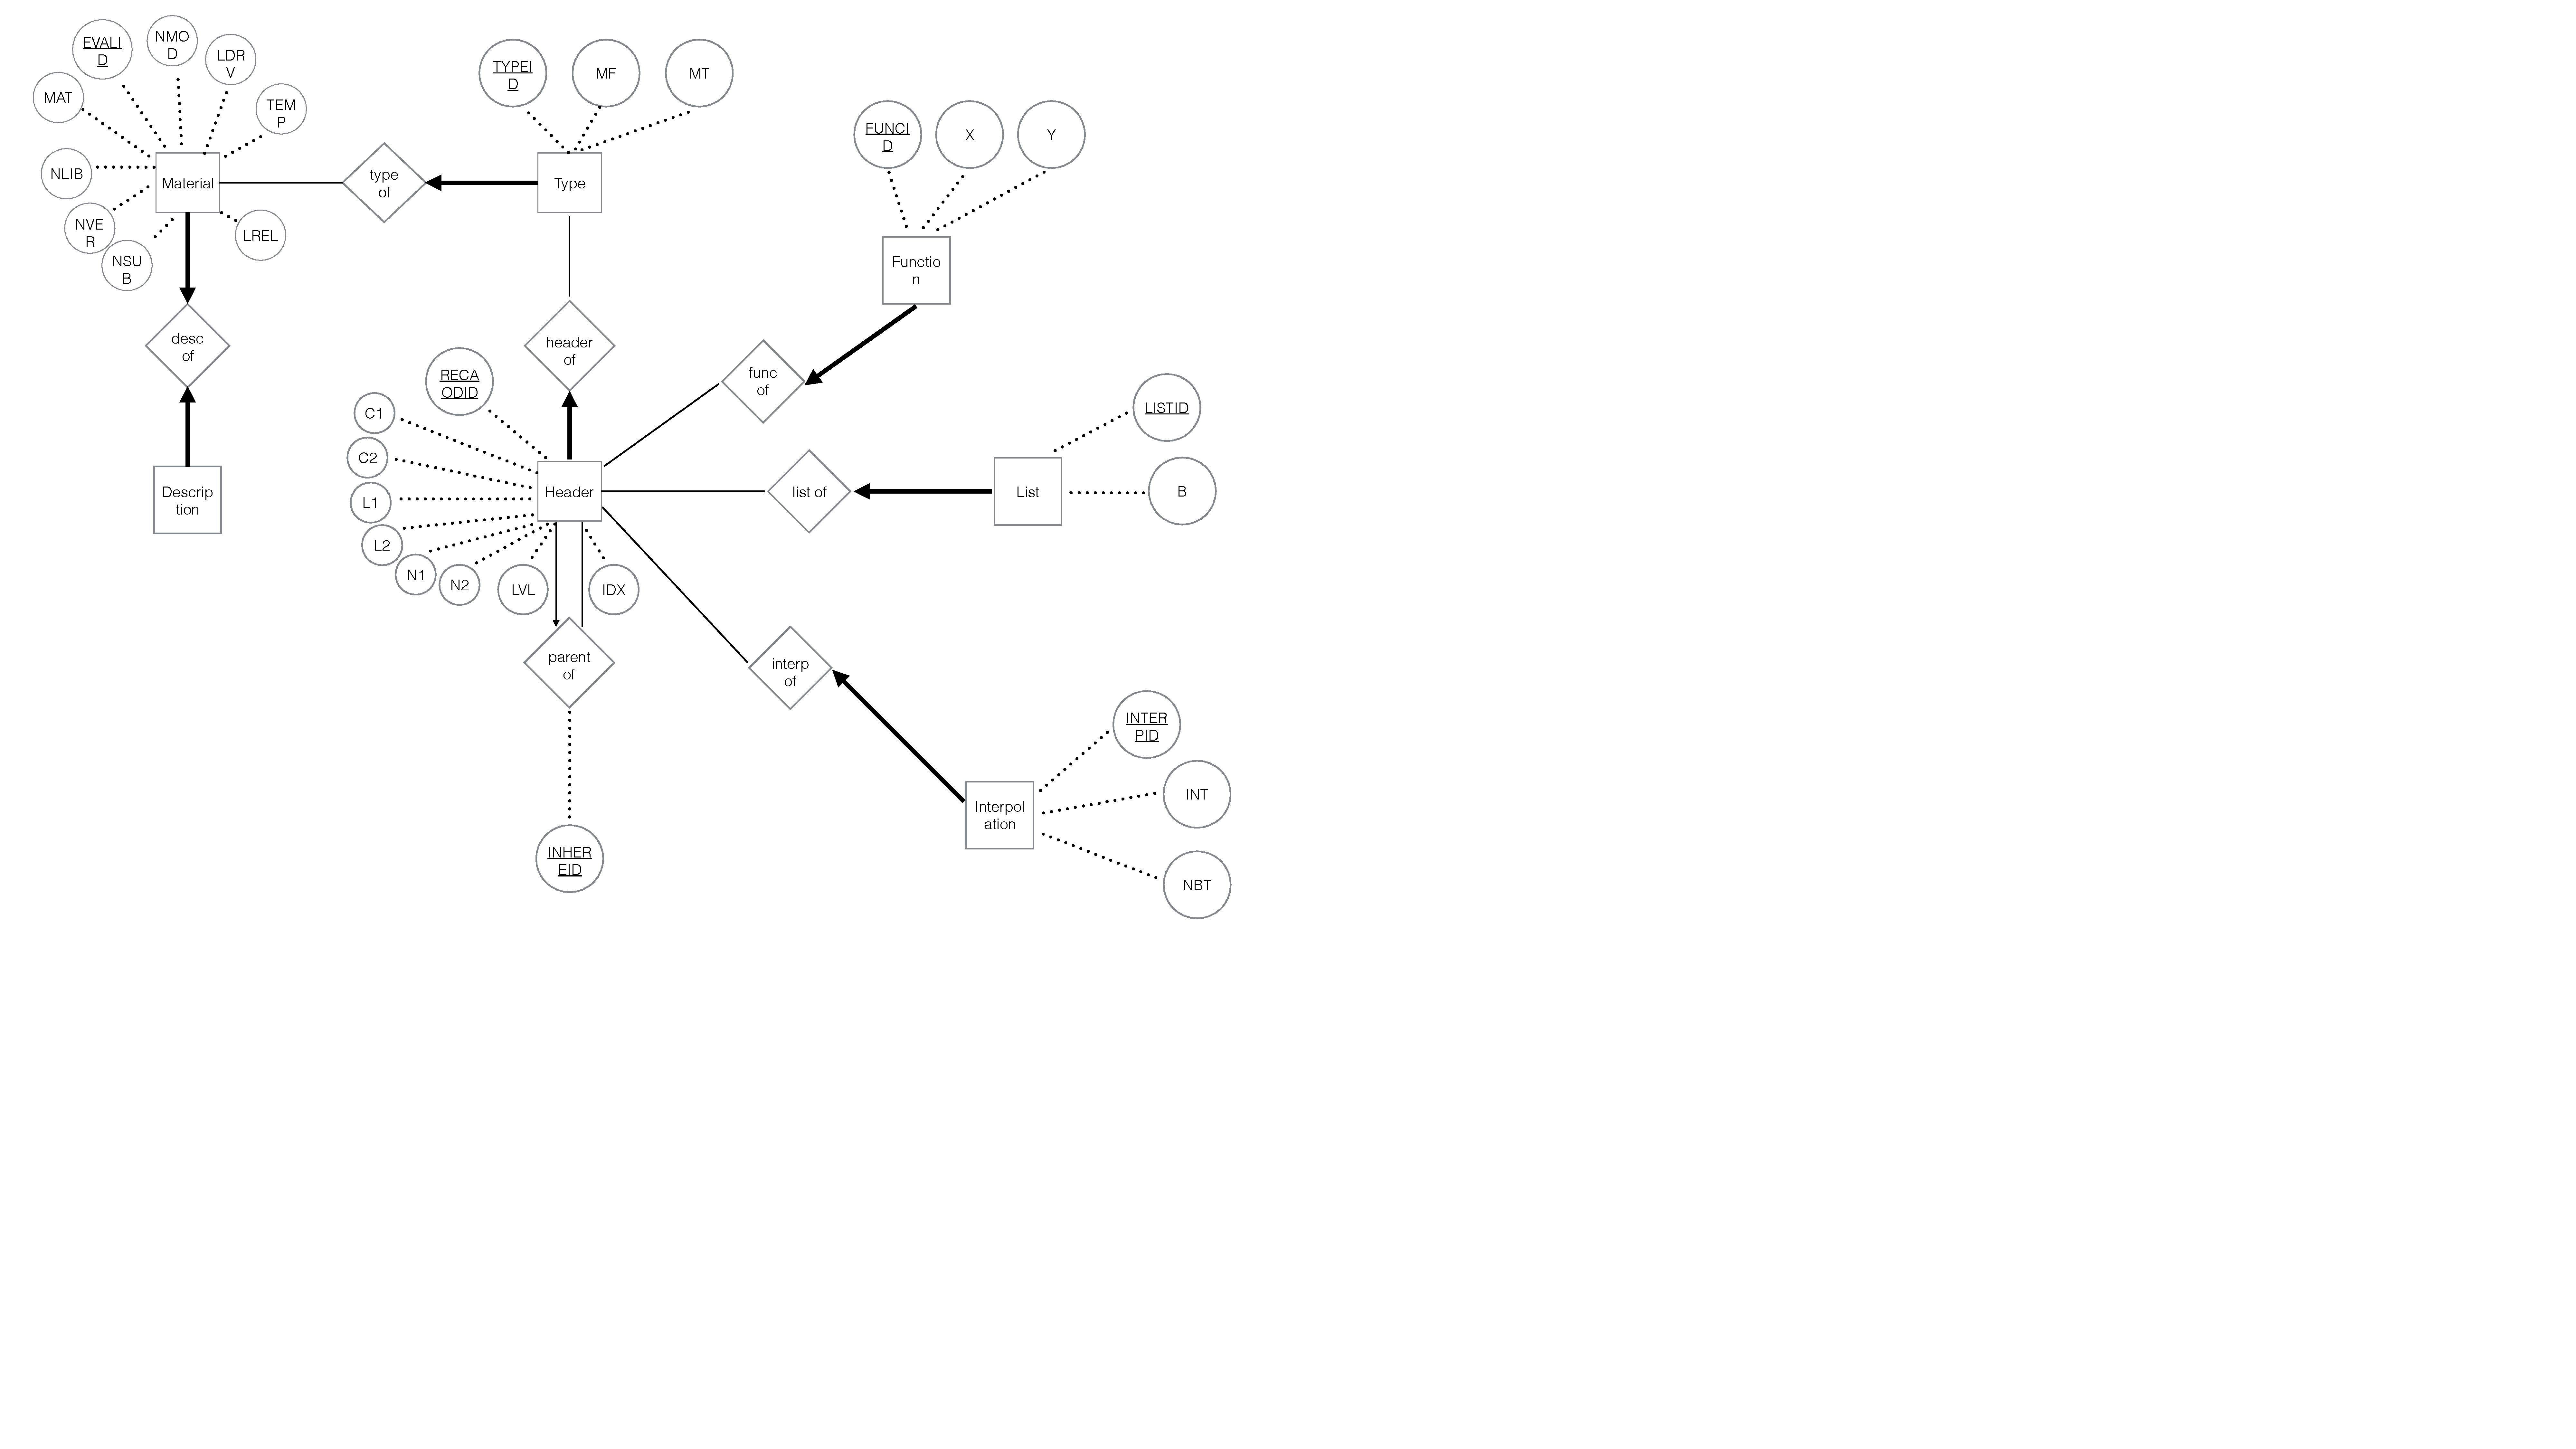
\includegraphics[scale=0.2]{./pics/endf-er-diagram.pdf}
\end{center}
\caption{ \label{fig:endf-6-record-tab2}
The ER diagram of the database}
\end{figure}

A header entity corresponds to a CONT record in the ENDF file, which contains six properties: C1, C2, L1, L2, N1, N2. In the ENDF text file, each CONT record is followed by any information for a list,  a one-dimensional function or a two dimensional function. The abstractions of function, list or interpolation entities, discussed later, are designated to describe a ENDF list, one-dimensional function, or a two dimensional function. Then in the ENDF file, a header entity is followed by a function, a list, an interpolation entity, or another header entity. An illustration of the file structure is shown in Figure \ref{fig:endf-header-inheritance}

\begin{figure}[h]
\begin{center}
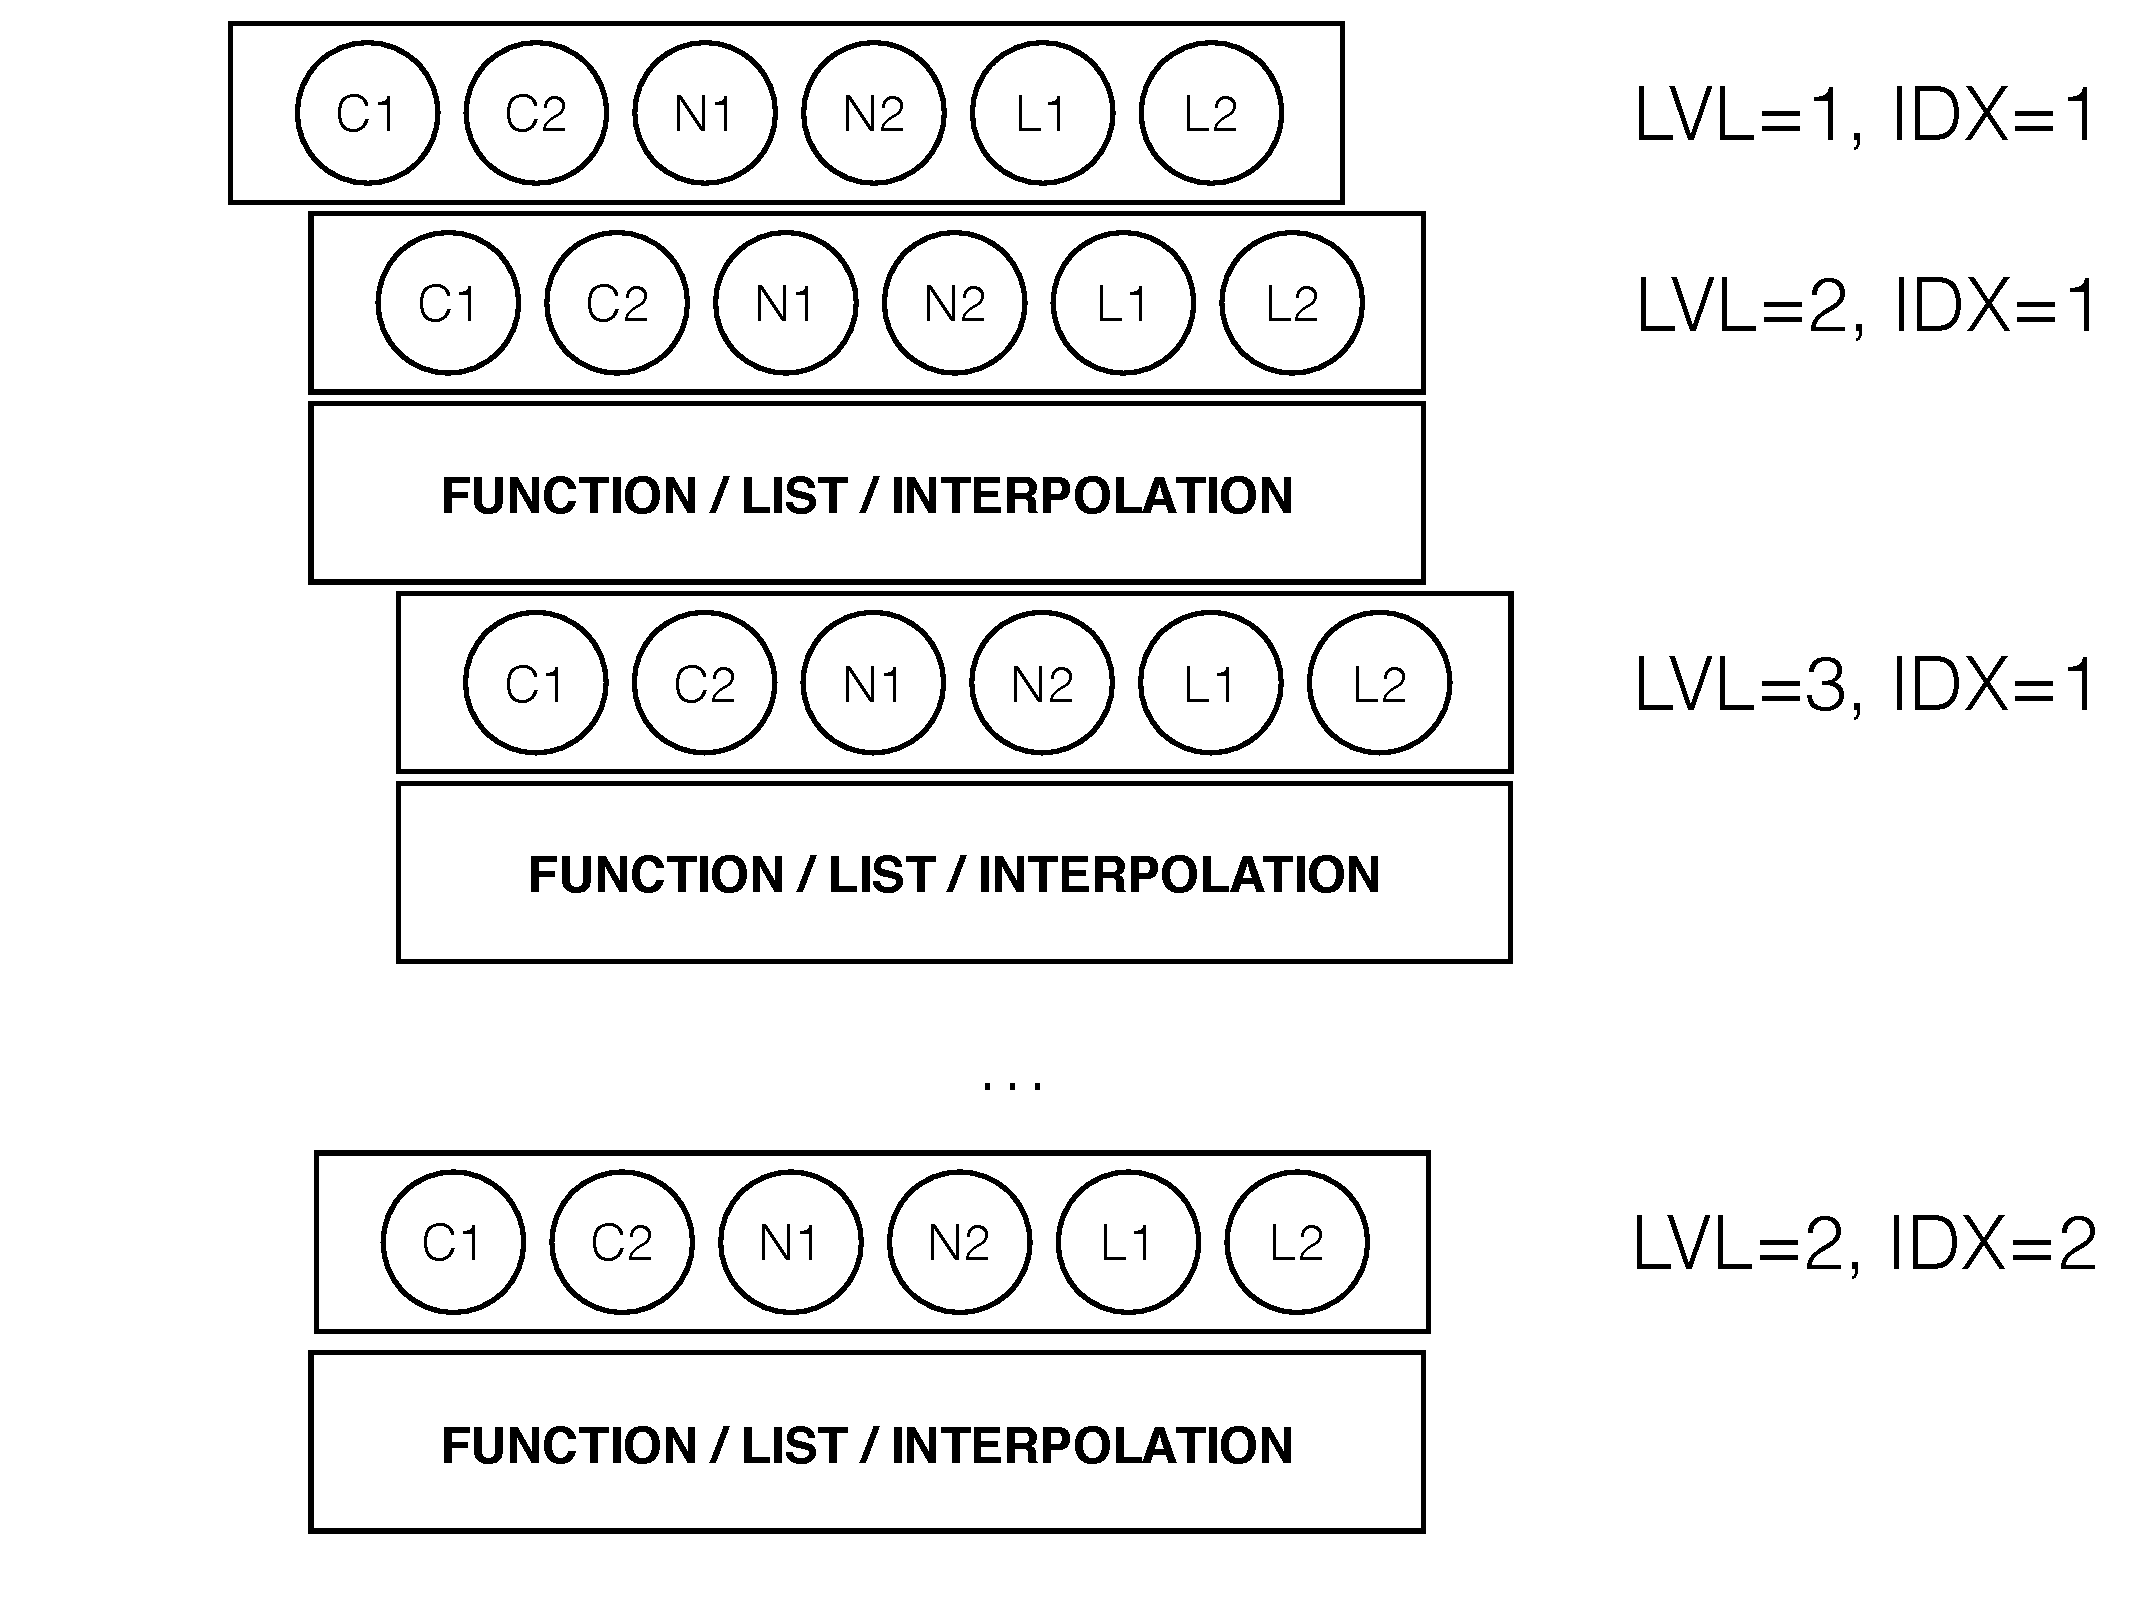
\includegraphics[scale=0.3]{./pics/endf-header-inheritance.pdf}
\end{center}
\caption{ \label{fig:endf-header-inheritance}
The header entities and the entities followed}
\end{figure}

Since a header entity could follow another header entity, there is an inherence relationship between the header entities. So we assign another two properties: the level (LVL) and the index (IDX) to indicate the parent-children relationship between headers and the brother and sister relationship between the header entities within a level. 

A function entity contains two properties x and y, which describe a one-dimensional function. A list entity contains a property B, which describes an array of data. An interpolation entity contains two properties: NBT and INT, which is used to describe the ENDF interpolation law. 

In the following sections, the database schema are given in more details.

\subsection{Material Table}
The material table contains important evaluation conditions for all evaluated data. According to the NJOY document, each evaluated data has a unique combination of MAT, NLIB, NVER, LREL, NSUB, NMOD, LDRV, and TEMP. We chose a self increasing integer EVALID as the primary key, which is generated at the time of inserting data into the database. The schema is shown in Program \ref{program:material_table_schema}.
\begin{program}[!htb]
\centering
\begin{verbatim} 
CREATE TABLE `Material_Table` (
	`EVALID`	INTEGER NOT NULL,
	`MAT`	INTEGER NOT NULL,
	`NLIB`	INTEGER NOT NULL,
	`NVER`	INTEGER NOT NULL,
	`LREL`	INTEGER NOT NULL,
	`NSUB`	INTEGER NOT NULL,
	`NMOD`	INTEGER NOT NULL,
	`LDRV`	INTEGER NOT NULL,
	`TEMP`	REAL NOT NULL,
	PRIMARY KEY(EVALID)
);
\end{verbatim}
\caption{ \label{program:material_table_schema}
SQL schema for material table}
\end{program}

\subsection{Description Table}
The description table includes additional evaluation information of the evaluated data. The EVALID from the material table is the primary key. The schema is shown in Program \ref{program:description_table_schema}.
\begin{program}[!htb]
\centering
\begin{verbatim} 
CREATE TABLE `Description_Table` (
	`EVALID`	INTEGER NOT NULL UNIQUE,
	`ZSYMAM`	TEXT,
	`ALAB`	TEXT,
	`EDATE`	TEXT,
	`AUTH`	TEXT,
	`REF`	TEXT,
	`DDATE`	TEXT,
	`RDATE`	TEXT,
	`ENDATE`	TEXT,
	`HSUB`	TEXT,
	`Summary`	TEXT,
	`Description`	TEXT,
	PRIMARY KEY(EVALID),
	FOREIGN KEY(`EVALID`) REFERENCES `Material_Table`(`EVALID`)
);
\end{verbatim}
\caption{ \label{program:description_table_schema}
SQL schema for description table}
\end{program}

\subsection{Type Table}
The type tables includes all file section paris. A self increasing integer TYPEID is automatically generated at the time of inserting data into the database and serve as the primary key. The schema is shown in Program \ref{program:type_table_schema}.

\begin{program}[!htb]
\centering
\begin{verbatim} 
CREATE TABLE `Type_Table` (
	`TYPEID`	INTEGER NOT NULL,
	`EVALID`	INTEGER NOT NULL,
	`MF`	INTEGER NOT NULL,
	`MT`	INTEGER NOT NULL,
	PRIMARY KEY(TYPEID),
	FOREIGN KEY(`EVALID`) REFERENCES `Material_Table`(`EVALID`)
);
\end{verbatim}
\caption{ \label{program:type_table_schema}
SQL schema for type table}
\end{program}

\subsection{Header Table}
The header table gives the header information for each record. A self increasing integer RECORDID is automatically generated at the time of inserting data into the database and serve as the primary key. The schema is shown in Program \ref{program:header_table_schema}.
\begin{program}[!htb]
\centering
\begin{verbatim} 
CREATE TABLE `Header_Table` (
	`RECORDID`	INTEGER NOT NULL,
	`TYPEID`	INTEGER NOT NULL,
	`C1`	REAL NOT NULL,
	`C2`	REAL NOT NULL,
	`L1`	REAL NOT NULL,
	`L2`	REAL NOT NULL,
	`N1`	REAL NOT NULL,
	`N2`	REAL NOT NULL,
	`LVL`	INTEGER NOT NULL,
	`IDX`	INTEGER NOT NULL,
	PRIMARY KEY(RECORDID),
	FOREIGN KEY(`TYPEID`) REFERENCES `Type_Table`(`TYPEID`)
);
\end{verbatim}
\caption{ \label{program:header_table_schema}
SQL schema for header table}
\end{program}

\subsection{Inheritance Table}
The inheritance table is designated to describe the inheritance relationship between the header tables, and the schema of which is shown in Program \ref{program:inherence_table_schema}.
\begin{program}[!htb]
\centering
\begin{verbatim} 
CREATE TABLE `Inheritance_Table` (
	`INHEREID`	INTEGER NOT NULL,
	`PARENTID`	INTEGER NOT NULL,
	`CHILDID`	INTEGER NOT NULL,
	PRIMARY KEY(INHEREID),
	FOREIGN KEY(`PARENTID`) REFERENCES `Header_Table`(`RECORDID`),
	FOREIGN KEY(`CHILDID`) REFERENCES `Header_Table`(`RECORDID`)
);
\end{verbatim}
\caption{ \label{program:inherence_table_schema}
SQL schema for inherence table}
\end{program}

\subsection{Function Table}
The function table records all one-dimensional functions x-y pairs. The RECORDID of a header table it associates with is the primary key. The schema of the function table is shown in Figure \ref{program:function_table_schema}.
\begin{program}[!htb]
\centering
\begin{verbatim} 
CREATE TABLE `Function_Table` (
	`FUNCID`	INTEGER NOT NULL,
	`RECORDID`	INTEGER NOT NULL UNIQUE,
	`X`	BLOB NOT NULL,
	`Y`	BLOB NOT NULL,
	PRIMARY KEY(FUNCID),
	FOREIGN KEY(`RECORDID`) REFERENCES `Header_Table`(`RECORDID`)
);
\end{verbatim}
\caption{ \label{program:function_table_schema}
SQL schema for function table}
\end{program}

\subsection{List Table}
The list table records all arrays of data in a list. The RECORDID of a header table it associates with is the primary key. The schema of the function table is shown in Figure \ref{program:list_table_schema}.
\begin{program}[!htb]
\centering
\begin{verbatim} 
CREATE TABLE `List_Table` (
	`LISTID`	INTEGER NOT NULL,
	`RECORDID`	INTEGER NOT NULL UNIQUE,
	`B`	BLOB NOT NULL,
	PRIMARY KEY(LISTID),
	FOREIGN KEY(`RECORDID`) REFERENCES `Header_Table`(`RECORDID`)
);
\end{verbatim}
\caption{ \label{program:list_table_schema}
SQL schema for list table}
\end{program}

\subsection{Interpolation Table}
The interpolation table records all ENDF interpolation rules. The RECORDID of a header table it associates with is the primary key. The schema of the function table is shown in Figure \ref{program:interpolation_table_schema}.
\begin{program}[!htb]
\centering
\begin{verbatim} 
CREATE TABLE `Interpolation_Table` (
	`INTERPID`	INTEGER NOT NULL,
	`RECORDID`	INTEGER NOT NULL UNIQUE,
	`INT`	BLOB NOT NULL,
	`NBT`	BLOB NOT NULL,
	PRIMARY KEY(INTERPID),
	FOREIGN KEY(`RECORDID`) REFERENCES `Header_Table`(`RECORDID`)
);
\end{verbatim}
\caption{ \label{program:interpolation_table_schema}
SQL schema for interpolation table}
\end{program}



%\section{Explicit Format Data-files}
%The information read from the database are too rudimentary and the meaning of the data are not disclosed explicitly. So we design the explicit format data-files to disclose the structural information of the nuclear data. The Google Protobuf format is used as a descriptive language for instantiating the nuclear data. In this section, we focus on the neutron data files.
%
%\subsection{Google Protobuf Message Format}
%The Google Protobuf protocol defines how to represent complex structured data. An example protocol message is shown in Program \ref{program:example_protocol}.
%
%\begin{program}[!htb]
%\centering
%\begin{verbatim} 
%message MessageName {
%modifier DataType variable = variable_index;
%}
%\end{verbatim}
%\caption{ \label{program:example_protocol}
%An example Google Protobuf protocol}
%\end{program}
%
%The 'messageName' variable is the name of the message or a structure. It is called a message because that the protocol file is used for sending data between computers in the Google cluster of servers. The 'modifier' field has three options, they are: required, repeated or optional, which modify the 'variable' after with type specified by 'DataType'. The data type can either be basic types such as a double precision floating number (double), a string (string), or  The 'variable\_index' is a unique integer for a variable in a message. This integer associates with the location of the variable when packed in an array of bytes.
%
%\subsection{Top Level Information for Neutron Data}
%The neutron data can be categorized into the resonance data (file 2), the reaction data (file 3), etc. The protocol is shown in Program \ref{program:top_level_neutron_data}.
%\begin{program}[!htb]
%\centering
%\begin{verbatim} 
%message NeutronData {
%	repeated Reaction reactions = 1;
%	repeated Resonance resonances = 2;
%}
%\end{verbatim}
%\caption{ \label{program:top_level_neutron_data}
%Google Protobuf protocol for top level information for neutron data}
%\end{program}
%
%\subsection{Fundamental ENDF data structures}
%The fundamental ENDF data structures include those for the ENDF tabulars and interpolation laws. The protocols are shown in Figure \ref{program:fundamental_endf_data_structure}.
%\begin{program}[!htb]
%\centering
%\begin{verbatim} 
%message TableInterpLaw {
%	required int64 INT = 1;
%	required int64 NBT = 2;
%}
%message TableDataPoint {
%	required double X = 1;
%	required double Y = 2;
%}
%message Table {
%	repeated TableInterpLaw interp_laws = 1;
%	repeated TableDataPoint data_points = 2;
%}
%\end{verbatim}
%\caption{ \label{program:fundamental_endf_data_structure}
%Google Protobuf protocol for fundamental ENDF data structures}
%\end{program}
%
%\subsection{Resonance Data}
%In this section, we disclose the design of resonance data. The resonance data are split into ranges of resonances. A resonance region can either be a resolved resonance region (RRR) or a unresolved resonance region (URR). 
%
%\subsubsection{Top Level Information for Resonance Data}
%The top level information for a resonance includes the atomic-mass number ZAI, the nuclide abundance ABN, the average fission width flag LFW, and an array of resonance ranges. The protocol is shown in Program \ref{program:top_level_neutron_data}.
%\begin{program}[!htb]
%\centering
%\begin{verbatim} 
%message Resonance {
%	required int64 ZAI = 1;
%	required double ABN = 2;
%	required int64 LFW = 3;
%	repeated ResonanceRange ranges = 4;
%}
%\end{verbatim}
%\caption{ \label{program:top_level_resonance_data}
%Google Protobuf protocol for top level information for resonance data}
%\end{program}
%
%\subsubsection{Top Level Information for Resonance Range}
%For each resonance range, there are many parameters to describe. The top level information is listed below in Program \ref{program:top_level_resonance_range}. The EL variable is the lower bound of the energy range, and EH is the upper bound of the energy range. LRU is an integer flag indicates which this is a RRR with LRU equals to 1 or URR with LRU equals to 2. LRF is an integer flag indicating the format of evaluation of the resonance parameters: Single-Level Breit-Wigner representation (SLBW) with LRF equals to 1. Multi-Level Breit-Wigner representation (MLBW) with LRF equals to 2, Reich-Moore representation (RM) with LRF equals to 3, Adler-Adler representation (AA) wth LRF equals to 4, and R-Matrix Limited representation (RML) with LRF equals to 7. NRO is the flag for indicating the energy dependence of the scattering radius: energy independent with NRO equals to 0, or energy dependent with NRO equals to 1. NAPS is the flag controls the use of channel radius and the scattering radius (AP). 
%
%Next, it is discussed here the information only applicable to the resolved resonance region with LRU equals to 1. SPI is the spin of the target nucleus. AP is the scattering radius in units ${10^{-12}}$cm. APE is an ENDF table to store the energy dependent scattering radius. LAD (for RM) is a flag indicating whether parameters can be used to calculate angular distributions. NLSC (for RM) is the number of angular moments used for converging calculations. LI (for AA) is the flag for controlling the kind of AA parameters. NX (for AA) is the number of sets of background constants. AWRI is the ratio of the mass of the isotope to the mass of a neutron, i.e. the atomic weight ratio. 
%
%\begin{program}[!htb]
%\centering
%\begin{verbatim} 
%message ResonanceRange {
%	required double EL = 1;
%	required double EH = 2;
%	required int64 LRU = 3;
%	required int64 LRF = 4;
%	required int64 NRO = 5;
%	required int64 NAPS = 6;
%
%	required double SPI = 11;
%	required double AP = 12;
%	required Table APE = 13;
%	required int64 LAD = 14;
%	required int64 NLSC = 15;
%
%	required int64 LI = 21;
%	required int64 NX = 22;
%	required double AWRI = 23;
%
%	required int64 LSSF = 31;
%	repeated double URRBES = 32;
%
%	required int64 IFG = 41;
%	required int64 KRM = 42;
%	required int64 KRL = 43;
%	repeated RMLParticlePair RMLPairs = 44;
%	repeated RMLSpin RMLSpins = 45;
%
%	repeated double AATotal = 51;
%	repeated double AAFission = 52;
%	repeated double AACapture = 53;
%
%	repeated AngularMomentum moments = 61;
%}
%\end{verbatim}
%\caption{ \label{program:top_level_resonance_range}
%Google Protobuf protocol for top level information for resonance range}
%\end{program}
%
%The additional defined data structures protocols are listed in Program \ref{program:additional_resonance_parameters}, Program \ref{program:additional_resonance_parameters_cont}, Program \ref{program:additional_resonance_parameters_cont2}, and Program
%\ref{program:additional_resonance_parameters_cont3}.
%
%\begin{program}[!htb]
%\centering
%\begin{verbatim} 
%message BreitWigner {
%	required double ER = 1;
%	required double AJ = 2;
%	required double GT = 3;
%	required double GN = 4;
%	required double GG = 5;
%	required double GF = 6;
%}
%message ReichMoore {
%	required double ER = 1;
%	required double AJ = 2;
%	required double GN = 3;
%	required double GG = 4;
%	required double GFA = 5;
%	required double GFB = 6;
%}
%message AAResonance {
%	required double DET = 1;
%	required double DWT = 2;
%	required double GRT = 3;
%	required double GIT = 4;
%	required double DEF = 5;
%	required double DWF = 6;
%	required double GRF = 7;
%	required double GIF = 8;
%	required double DEC = 9;
%	required double DWC = 10;
%	required double GRC = 11;
%	required double GIC = 12;
%}
%message AdlerAdler {
%	required double AJ = 1;
%	repeated AAResonance resonaces = 2;
%}
%\end{verbatim}
%\caption{ \label{program:additional_resonance_parameters}
%Google Protobuf protocol for top level information for  addition resonance paramters}
%\end{program}
%
%\begin{program}[!htb]
%\centering
%\begin{verbatim} 
%message UrrA {
%	required double D = 1;
%	required double AJ = 2;
%	required double AMUN = 3;
%	required double GNO = 4;
%	required double GG = 5;
%}
%message UrrB {
%	required double L = 1;
%	required double MUF = 2;
%	required double D = 3;
%	required double AJ = 4;
%	required double AMUN = 5;
%	required double GNO = 6;
%	required double GG = 7;
%	repeated double GF = 8;
%}
%message UrrC {
%	required double AJ = 1;
%	required int64 INT = 2;
%	required double AMUX = 3;
%	required double AMUN = 4;
%	required double AMUG = 5;
%	required double AMUF = 6;
%	repeated double ES = 7;
%	repeated double D = 8;
%	repeated double GX = 9;
%	repeated double GNO = 10;
%	repeated double GG = 11;
%	repeated double GF = 12;
%}
%message AngularMomentum {
%	required double AWRI = 1;
%	required double QX = 2;
%	required double L = 3;
%	required int64 LRX = 4;
%	required double APL = 5;
%	repeated BreitWigner BWTables = 6;
%	repeated ReichMoore RMTables = 7;
%	repeated AdlerAdler AATables = 8;
%	repeated UrrA URRATables = 9;
%	repeated UrrB URRBTables = 10;
%	repeated UrrC URRCTables = 11;
%}
%\end{verbatim}
%\caption{ \label{program:additional_resonance_parameters_cont}
%Google Protobuf protocol for top level information for  addition resonance parameters (Continue)}
%\end{program}
%
%\begin{program}[!htb]
%\centering
%\begin{verbatim} 
%message RMLParticlePair {
%	required double MA = 1;
%	required double MB = 2;
%	required int64 ZA = 3;
%	required int64 ZB = 4;
%	required int64 IA = 5;
%	required int64 IB = 6;
%	required double Q = 7;
%	required int64 PNT = 8;
%	required int64 SHF = 9;
%	required int64 MT = 10;
%	required double PA = 11;
%	required double PB = 12;
%}
%message RMLChannel {
%	required double IPP = 1;
%	required double L = 2;
%	required double SCH = 3;
%	required double BND = 4;
%	required double APE = 5;
%	required double APT = 6;
%
%	required int64 LBK = 11;
%	required int64 LPS = 12;
%	required Table RBR = 13;
%	required Table RBI = 14;
%	required Table PSR = 15;
%	required Table PSI = 16;
%	required double R0 = 17;
%	required double S0 = 18;
%	required double R1 = 19;
%	required double S1 = 20;
%	required double R2 = 21;
%	required double EU = 22;
%	required double ED = 23;
%	required double GA = 24;
%}
%\end{verbatim}
%\caption{ \label{program:additional_resonance_parameters_cont2}
%Google Protobuf protocol for top level information for  addition resonance parameters (Continue)}
%\end{program}
%
%\begin{program}[!htb]
%\centering
%\begin{verbatim} 
%message RMLResonance {
%	required double ER = 1;
%	repeated double GAMS = 2;
%}
%message RMLSpin {
%	required double AJ = 1;
%	required double PJ = 2;
%	required int64 KBK = 3;
%	required int64 KPS = 4;
%	repeated RMLChannel RMLChannels = 5;
%	repeated RMLResonance RMLResonances = 6;
%}
%\end{verbatim}
%\caption{ \label{program:additional_resonance_parameters_cont3}
%Google Protobuf protocol for top level information for  addition resonance parameters (Continue)}
%\end{program}

%\subsection{Reaction Data}

\clearpage
\section{C++ Data Structure \& Application Interfaces}
The program is implemented native in C++ programming language, so in this section, we discuss the data structures first then the application interfaces.

\subsection{Data Structure}


\subsection{Application Interfaces (APIs)}
\begin{program}[!htb]
\centering
\begin{verbatim} 
class NDLS {
public:
    NDLS(const std::string& dbFilepath);
    ~NDLS();
    
    bool open(const std::string& dbFilepath);
    void close();
    bool insertENDFFile(const std::string& endfFilepath);
}
\end{verbatim}
\caption{ \label{program:ndls_cpp_api}
C++ public APIs for NDLS module}
\end{program}


\chapter{LS: Linearization System} \label{chap:ls}
In this chapter we discuss an important topic in converting complex function into its linearized form. This is important since, the linearized function costs less computations. For the importance in its own, we use a whole chapter to discuss it.

\chapter{XLS: Cross Section Linearization System} \label{chap:xls}
The given cross sections in the reactions may not be linearized. As a result, they can be easily summed or accumulated. 

\section{Algorithm}
The ENDF interpolation tabular data points are divided into regions, each of which uses an integer from 1 to 5 to indicate the method of interpolation. 

\subsection{Histogram}
If the interpolation law number is 1, the method of interpolation represents a histogram. The points on the region boundaries will remain the same, and each point internal to the region will be accompanied by another point with a $y$ value equal to the previous point. 

\subsection{Linear-Linear Interpolation}
If the interpolation law number is 2, the method of interpolation is linear to linear. All points will remain the same. No modifications will be applied.

\subsection{Other Laws of Interpolation}
If the interpolation law number betweens 3 and 5, additional data points may be necessary to be inserted into the region to make the error of linearization below a certain level of requirement, for example $0.1\%$. The algorithm applied is called the method of inverted stack. 

\subsection{Removal of Duplicated Points}
Sometimes, the data points after the linearization may have duplications. That is the case that for two points: $(x_1,y_1)$ and $(x_2,y_2)$, we have:
\begin{eqnarray}
x_1 &=& x_2,\\
|y_1-y_2| &<& \epsilon,
\end{eqnarray}
where $\epsilon$ is small value such as $1\times10^{-10}$ barn.

\section{C++ Data Structures \& APIs}
The XLS class has a static method called `linearizeENDFInterpFunc', which takes a ENDF interpolation table function and return a vector of cross section data points.
\begin{verbatim}
struct XLSXsecPair {
    double energyEv  = 0.;
    double sigmaBarn = 0.;
};

// Discontinuity of cross section may present
struct XLSXsec {
    std::vector<XLSXsecPair> xspairs;
};

// The cross section linearization system will take
// an ENDFInterpolationFunction representation
// of a cross section data, and linearlize it
// into an XLSXsec data format, the tolerance in the fraction
// of the relative error is given
class XLS {
public:
    static XLSXsec linearizeENDFInterpFunc
    (const ENDFInterpolationFunction& endf, double tol);
};
\end{verbatim}

\chapter{XRS: Cross Section Reconstruction System} \label{chap:xrs}
The evaluated nuclear data are not easily used by the neutron transport softwares. So further processing are necessary. One important step is to discretize the cross sections on an energy grid with the cross sections linearized on it. In this chapter, we first discuss the topic of resonance cross section reconstruction and then how to combine the resonance with tabulated cross sections.

\section{Resolved Resonance}
In this section, we discuss the mathematical theories behind cross section evaluations and the method of linearization. First, we focus on the resolved resonance regions. Second, the unresolved resonance region is discussed. 

\subsection{SLBW: Single-level Breit-Wigner}
The Single-Level Breit-Wigner (SLBW) is the most simple ways of describing the resonance peaks. First the format of the data provided by the ENDF database is presented. Second, the mathematical theories behind for how to evaluating cross sections at a given energy is discussed. Third, how to write a computer algorithm is discussed.

\subsubsection{Data Format}
The data given from the ENDF database are discussed now. First, we list some scalar variables:
\\\\
\begin{small}
\begin{tabular}{l l l L{6cm}}
Variable Name & ENDF Name & Type & Meaning \\\hline
$I$ & SPI & floating & the total spin \\
$\hat{a}$ & AP & floating & scattering radius in units of $10^{-12}$ cm \\
$N$ & NLS & integer & the number of neutron orbital angular momentum \\
$A$ & AWRI & floating & the ratio of the mass of the isotope to that of a neutron \\
$a$ & N/A & floating & the channel radius \\
$f$ & NAPS & integer & radius choice flag\\
\end{tabular}
\end{small}
\\\\
There are $N$ angular momenta. For each angular momentum $l_i$ with $1\leq i\leq N$, there are some variables are defined depending on the index $i$:
\\\\
\begin{small}
\begin{tabular}{l l l L{6cm}}
Variable Name & ENDF Name & Type & Meaning \\\hline
$l_i$ & L & floating & angular momentum at index $i$\\
$M_i$ & NRS & integer & number of resolved resonances for $l_i$ \\
$Q_i$ & QX & floating & the Q-value used in calculating the penetrability factor \\
\end{tabular}
\end{small}
\\\\
There are some variables defined for the resonance defined at the resonance index $1\leq r\leq M_i$ for the angular momentum $l_i$. They are listed in the following table:
\\\\
\begin{small}
\begin{tabular}{l l l L{6cm}}
Variable Name & ENDF Name & Type & Meaning \\\hline
$E_{ir}$ & ER & floating & the resonance energy measured in the laboratory system for $r$th resonance and angular momentum $l_i$ \\
$J_{ir}$ & AJ & floating & the spin for $r$th resonance and angular momentum $l_i$\\
$\Gamma_{ir}^0$ & GT & floating & the resonance total width evaluated at energy $E_{ir}$ \\
$\Gamma_{n,ir}^0$ & GN & floating & the neutron width evaluated at energy $E_{ir}$ \\
$\Gamma_{\gamma,ir}^0$ & GG & floating & radiation width evaluated at energy $E_{ir}$ \\
$\Gamma_{f,ir}^0$ & GF & floating & fission width evaluated at energy $E_{ir}$\\
$\sigma_{m,ir}$ & N/A & floating & maximum cross section at energy $E_{ir}$
\end{tabular}
\end{small}
\\\\

\subsubsection{Mathematical Theory}
There are several commonly used types of representations for describing the resolved resonances. The first one is the Single-Level Breit-Wigner Representation (SLBW), the resonance elastics cross section ($\sigma_n$), the fission cross section ($\sigma_f$), the capture cross section ($\sigma_\gamma$), and the potential scattering cross section ($\sigma_p$) are given by:
\begin{eqnarray}
\sigma_n (E) &=& \sigma_p(E) \nonumber\\[1ex]
&& + \sum_{i=1}^{N} \sum_{r=1}^{M_i} \sigma_{m,ir}(E)\left\{\left[\cos2\phi_{l_i}(E)-(1-\frac{\Gamma_{n,ir}(E)}{\Gamma_{ir}(E)})\right]\psi(x_{ir}(E))\right.\nonumber\\
&& \left. + \sin2\phi_{l_i}(E)\frac{}{}\chi(x_{ir}(E))\right\}, \\
\sigma_{f} (E) &=& \sum_{i=1}^{N}\sum_{r=1}^{M_i} \sigma_{m,ir}(E) \frac{\Gamma_{f,ir}^0}{\Gamma_{ir}(E)} \psi(x_{ir}(E)),\\
\sigma_{\gamma}(E) &=&  \sum_{i=1}^{N}\sum_{r=1}^{M_i} \sigma_{m,ir}(E) \frac{\Gamma_{\gamma,ir}^0}{\Gamma_{ir}(E)} \psi(x_{ir}(E)),\\
\sigma_p (E) &=& \sum_{i=1}^{N} \frac{4\pi}{k(E)^2}(2l_i+1)\sin^2\phi_{l_i}(E),
\end{eqnarray}
where the given quantities are:
\begin{eqnarray}
E &=& \mbox{incident laboratory energy in units of eV},\\
A &=& \mbox{isotope weight ratio to neutron}, \\
N &=& \mbox{number of angular momentum}, \\
f &=& \mbox{radius choice flag either 0 or 1}, \\
l_i &=& i\mbox{th angular momentum},\; 1\leq i\leq N,\\
M_i &=& \mbox{number of resonance associated with }l_i,\\ 
\hat{a} &=& \mbox{scattering radius}, \\
J_{ir} &=& \mbox{spin for angular momentum }l_i\mbox{ and $r$th resonance }, \nonumber\\
&&1\leq i\leq N,\;1\leq r\leq M_i,\\
I &=& \mbox{total spin},\\
E_{ir} &=& \mbox{energy at the center of resonance},  \;1\leq i\leq N,\;1\leq r\leq M_i,\\
\Gamma_{ir}^0 &=& \mbox{resonance total width at } E_{ir}, \;1\leq i\leq N,\;1\leq r\leq M_i,\\
\Gamma_{n,ir}^0 &=& \mbox{resonance neutron width at } E_{ir}, \;1\leq i\leq N,\;1\leq r\leq M_i,\\
\Gamma_{\gamma,ir}^0 &=& \mbox{resonance capture width at } E_{ir}, \;1\leq i\leq N,\;1\leq r\leq M_i,\\
\Gamma_{f,ir}^0 &=& \mbox{resonance fission width at } E_{ir}, \;1\leq i\leq N,\;1\leq r\leq M_i,
\end{eqnarray}
The energy dependent resonance widths are:
\begin{eqnarray}
\Gamma_{n,ir}(E) &=& \frac{P_{l_i}(E)\Gamma_{n,ir}^0}{P_{l_i}(|E_{ir}|)}, \;1\leq i\leq N,\;1\leq r\leq M_i,\\
\Gamma_{ir}(E) &=& \Gamma_{n,ir}(E) + \Gamma_{ir}^0 - \Gamma_{n,ir}^0, \;1\leq i\leq N,\;1\leq r\leq M_i,
\end{eqnarray}
and the derived quantities are:
\begin{eqnarray}
k(E) &=& (2.196771\times10^{-3})\frac{A}{A+1}\sqrt{E},\\
g_{ir} &=& \frac{2J_{ir}+1}{4I+2},\; 1\leq i\leq N,\;1\leq r\leq M_i,\\
\sigma_{m,ir}(E) &=& \frac{4\pi}{k(E)^2}g_{ir}\frac{\Gamma_{n,ir}(E)}{\Gamma_{ir}(E)},\; 1\leq i\leq N,\;1\leq r\leq M_i,\\
a &=& \left\{\begin{array}{l l}0.123\;A^{1/3}+0.08, & f=0 \\\hat{a}, & f=1 \end{array}\right.,\\
\rho(E) &=& k(E)a,\\
\hat{\rho}(E) &=& k(E)\hat{a},\\
E_{ir}'(E) &=& E_{ir}+\frac{S_{l_1}(|E_{ir}|)-S_{l_i}(E)}{2P_{l_i}(|E_{ir}|)}\Gamma_{n,ir}^0,\; 1\leq i\leq N,\;1\leq r\leq M_i,\\
x_{ir}(E) &=& \frac{2(E-E_{ir}'(E))}{\Gamma_{ir}(E)},\; 1\leq i\leq N,\;1\leq r\leq M_i,\\
\psi(x) &=& \frac{1}{1+x^2},\\
\chi(x) &=& \frac{x}{1+x^2}.
\end{eqnarray}
The penetration factors are defined here:
\begin{eqnarray}
P_0(E) &=& \rho(E),\\
P_1(E) &=& \frac{\rho(E)^3}{1+\rho(E)^2},\\
P_2(E) &=& \frac{\rho(E)^5}{9+3\rho(E)^2+\rho(E)^4},\\
P_3(E) &=& \frac{\rho(E)^7}{225+45\rho(E)^2+6\rho(E)^4+\rho(E)^6},\\
P_4(E) &=& \frac{\rho(E)^9}{11025+1575\rho(E)^2+135\rho(E)^4+10\rho(E)^6+\rho(E)^8}.
\end{eqnarray}
The phase shifts are defined here:
\begin{eqnarray}
\phi_0(E) &=& \hat{\rho}(E),\\
\phi_1(E) &=& \hat{\rho}(E)-\tan^{-1}\hat{\rho}(E),\\
\phi_2(E) &=& \hat{\rho}(E)-\tan^{-1}\frac{3\hat{\rho}(E)}{3-\hat{\rho}(E)^2},\\
\phi_3(E) &=& \hat{\rho}(E)-\tan^{-1}\frac{15\hat{\rho}(E)-\hat{\rho}(E)^3}{15-6\hat{\rho}(E)^2},\\
\phi_4(E) &=& \hat{\rho}(E)-\tan^{-1}\frac{105\hat{\rho}(E)-10\hat{\rho}(E)^3}{105-45\hat{\rho}(E)^2+\hat{\rho}(E)^4}.
\end{eqnarray}
The shift factors are defined here:
\begin{eqnarray}
S_0(E) &=& 0,\\
S_1(E) &=& -\frac{1}{1+\rho(E)^2},\\
S_2(E) &=& -\frac{18+3\rho(E)^2}{9+3\rho(E)^2+\rho(E)^4},\\
S_3(E) &=& -\frac{675+90\rho(E)^2+6\rho(E)^4}{225+45\rho(E)^2+6\rho(E)^4+\rho(E)^6},\\
S_4(E) &=& -\frac{44100+4725\rho(E)^2+270\rho(E)^4+10\rho(E)^6}{11025+1575\rho(E)^2+135\rho(E)^4+10\rho(E)^6+\rho(E)^8}.
\end{eqnarray}

Plug in all definitions into the formula for cross sections. We have simplified versions:
\begin{eqnarray}
\sigma_{n}(E)  &=& \sigma_p(E) + \frac{\pi}{k(E)^2}\sum_{i=1}^{N}\sum_{r=1}^{M_i}g_{ir}\nonumber\\
&& \frac{\Gamma_{n,ir}(E)^2-2\Gamma_{n,ir}(E)\Gamma_{ir}(E)\sin^2\phi_{l_i}(E)+2(E-E_{ir}'(E))\sin2\phi_{l_i}(E)}{\frac{1}{4}\Gamma_{ir}^2(E)+(E-E_{ir}'(E))^2}\nonumber\\
&&\\
\sigma_{\gamma}(E) &=& \frac{\pi}{k(E)^2}\sum_{i=1}^{N}\sum_{r=1}^{M_i}g_{ir}\frac{\Gamma_{n,ir}(E)\Gamma_{\gamma,ir}^0}{\frac{1}{4}\Gamma_{ir}^2(E)+(E-E_{ir}'(E))^2},\\
\sigma_{f}(E) &=& \frac{\pi}{k(E)^2}\sum_{i=1}^{N}\sum_{r=1}^{M_i}g_{ir}\frac{\Gamma_{n,ir}(E)\Gamma_{f,ir}^0}{\frac{1}{4}\Gamma_{ir}^2(E)+(E-E_{ir}'(E))^2},\\
\sigma_{p}(E) &=& \sum_{i=1}^{N} \frac{4\pi}{k(E)^2}(2l_i+1)\sin^2\phi_{l_i}(E).
\end{eqnarray}


\subsection{MLBW: Multilevel Breit-Wigner}

\subsubsection{Data Format}
The data required by MLBW calculation are the same as that of SLBW.


\subsubsection{Mathematical Theory}



\subsection{R-M: Reich Moore}

\subsubsection{Data Format}

\subsubsection{Mathematical Theory}







\chapter{DBS: Doppler Broadening System} \label{chap:dbs}
Doppler broadening is an important physical phenomena need to take consideration for neutron transport calculation to get the collision probability correct. We first discuss the mathematical background of this issue, and then give the theory behind the widely used SIGMA1 method.
\section{Mathematical Background of Doppler Broadening}
Let $\vec{v}$ be the velocity of the neutron, let $\vec{V}$ be the velocity of the target nucleus, then we can define an averaged collision cross section for target nuclide moving with a probability $f(\vec{V})$.
\begin{eqnarray}
\int_{R^3}f(\vec{V})d\vec{V}&=&1,
\end{eqnarray}
\noindent where if $\vec{V}=(x,y,z)$ or $\vec{V}=(r\cos\theta\sin\phi,r\sin\theta\sin\phi,r\cos\phi)$, for a general function $K(\vec{V})=K(x,y,z)$:
\begin{eqnarray}
\int_{R^3}K(\vec{V})d\vec{V}&=&\int_{0}^\infty\int_{0}^\infty\int_{0}^\infty K(\vec{V})dxdydz,\\
\int_{R^3}K(\vec{V})d\vec{V}&=&\int_{0}^\infty\int_{0}^{\pi}\int_{0}^{2\pi} K(\vec{V}) r^2\sin\phi d\theta d\phi dr,
\end{eqnarray}
\noindent the averaged cross section is:
\begin{eqnarray}
\bar{\sigma}(\vec{v})&=&\frac{1}{|\vec{v}|}\int_{R^3}|\vec{v}-\vec{V}|\sigma(|\vec{v}-\vec{V}|)f(\vec{V})d\vec{V}.
\end{eqnarray}
\noindent In the thermal motion case, the distribution function $f$ follows the free-gas thermal motion law, which at temperature $T$ is:
\begin{eqnarray}
f(\vec{V})&=&f^{*}(|\vec{V}|, T)=(\frac{M}{2\pi k T})^{3/2}e^{-M|\vec{V}|^2/2kT},
\end{eqnarray}
\noindent which depends only on the magnitude of $\vec{V}$. In this case we are able to define a cross section only depends on the magnitude of neutron velocity $\vec{v}$:
\begin{eqnarray}
\bar{\sigma}(|\vec{v}|,T)&=&\frac{1}{|\vec{v}|}\int_{R^3}|\vec{v}-\vec{V}|\sigma(|\vec{v}-\vec{V}|)f^{*}(|\vec{V}|, T)d\vec{V}.
\end{eqnarray}
\noindent If we define $v_r=|\vec{v}-\vec{V}|$, and denote $v$ and $V$ as the speed of $\vec{v}$ and $\vec{V}$:
\begin{eqnarray}
v&=&|\vec{v}|,\\
V&=&|\vec{V}|.
\end{eqnarray}
\noindent It is possible to rewrite the integral in scalar quantities as:
\begin{eqnarray}
\bar{\sigma}(v,T)&=&\frac{2\pi}{v^2}\int_0^{\infty}\int_{|v-V|}^{v+V}v_r^2\sigma(v_r)Vf^{*}(V,T)dv_rdV.
\end{eqnarray}
\noindent Change the order of integration, we get:
\begin{eqnarray}
\bar{\sigma}(v,T)&=&\frac{2\pi}{v^2}\int_0^{\infty}\int_{|v-v_r|}^{v+v_r}v_r^2\sigma(v_r)Vf^{*}(V,T)dVdv_r.
\end{eqnarray}
\noindent If we define the thermal speed $v_{th}=\sqrt{kT/M}$, $\omega=v/\sqrt{2}v_{th}$, and $\omega_r=v_r/\sqrt{2}v_{th}$:
\begin{eqnarray}
\bar{\sigma}(\omega,T)&=&\frac{1}{\omega^2\sqrt{\pi}}\int_0^{\infty}\omega_r^2\sigma(\omega_r)\left(e^{-(\omega-\omega_r)^2}-e^{-(\omega+\omega_r)^2}\right)d\omega_r.
\end{eqnarray}
\noindent In terms of the more frequently used energy quantities of neutron $E=\frac{1}{2}mv^2$, where $m$ is the neutron mass. We define the additional quantities:
\begin{eqnarray}
\alpha &=& \frac{M}{2kT},\\
x &=& \sqrt{\alpha}\,v = \sqrt{\alpha \frac{2E}{m}}=\sqrt{\frac{ME}{mkT}},
\end{eqnarray}
where $x$ is dimensionless. We define $\sigma(x,T)$ as the cross section as a function of the variable $x$ and temperature $T$, the formula is rewrite as:
\begin{eqnarray}
x^2\sigma(x,T) &=& \frac{1}{\sqrt{\pi}}\int_{0}^{\infty}x_r^2\sigma(x_r,0)\left(e^{-(x-x_r)^2}-e^{-(x+x_r)^2}\right)dx_r,
\end{eqnarray}
in which we have $x=\omega$ and $x_r=\omega_r$. In a more general case, if we start at temperature $T_1$ and want to get doppler broadened cross section at temperature $T_2$, and define $\alpha=M/2k(T_2-T_1)$, and $x=\sqrt{ME/mk(T_2-T_1)}$, we have:
\begin{eqnarray}
x^2\sigma(x,T_2) &=& \frac{1}{\sqrt{\pi}}\int_{0}^{\infty}x_r^2\sigma(x_r,T_1)\left(e^{-(x-x_r)^2}-e^{-(x+x_r)^2}\right)dx_r.
\end{eqnarray}
For simplicity, if we change the variable $x_r,x$ by $x,y$, we have:
\begin{eqnarray}
y^2\sigma(y,T_2) &=& \frac{1}{\sqrt{\pi}}\int_{0}^{\infty}x^2\sigma(x,T_1)\left(e^{-(y-x)^2}-e^{-(y+x)^2}\right)dx,
\end{eqnarray}
which is the formula we usually see in the textbooks.

\section{Theory of SIGMA1 Method}
The SIGMA1 method is probably the most widely used algorithm in the doppler broadening codes. It starts from a linearly interpolated cross section data points, which appears in the PENDF format in the NJOY system. We first define this linearly interpolated data points and derive the algorithm on it.
\subsection{Grid for Data Points}
Given the `cold'  cross section on a $x$ grid $(x_n,\sigma_n),n=1\dots N$ with additional data points:
\begin{eqnarray}
x_0 &=& 0,\\
x_{N+1} &=& \infty.
\end{eqnarray}
Let the cross section have a $1/x$ interpolation below the given data points, i.e. in the interval $(0,x_1]$/ The cross section is constant above the given data points, i.e. in the interval $(x_N,\infty)$. Therefore, the cross sections as a function of $x$ at the cold temperature $T_1$ are given by:
\begin{eqnarray}
\sigma(x,T_1)&=&\left\{
\begin{array}{r @{\;:\;} l}
\frac{x_1\sigma_1}{x} & 0<x\leq x_1\\
\sigma_n+s_n(x^2-x_n^2) & x_n<x\leq x_{n+1},\;\;1\leq n\leq {N-1}\\
\sigma_N & x_N<x<\infty
\end{array}\right.,
\label{eq:dbxsec}
\end{eqnarray}
where the slope is given by:
\begin{eqnarray}
s_n &=& \frac{\sigma_{n+1}-\sigma_n}{x_{n+1}^2-x_n^2},\;\;1\leq n\leq {N-1}.
\end{eqnarray}
\subsection{SIGMA1 Algorithm}
The doppler broadened cross section at `hot' temperature $T_2$ is given by the formula:
\begin{eqnarray}
\sigma(y,T_2) &=& \sigma^{*}(y,T_2) - \sigma^{*}(-y,T_2),\\[1ex]
\sigma^{*}(y,T_2) &=& \frac{1}{\sqrt{\pi}\,y^2}\int_{0}^{\infty}x^2\,\sigma(x,T_1)\,e^{-(x-y)^2}dx.
\end{eqnarray}
Plug in the formula Equation (\ref{eq:dbxsec}) for interpolated `cold' cross section formula:
\begin{eqnarray}
\sigma^{*}(y,T_2) &=& x_1\sigma_1\frac{1}{\sqrt{\pi}\,y^2}\int_{0}^{x_1}x\,e^{-(x-y)^2}dx+\nonumber\\
&&\frac{1}{\sqrt{\pi}\,y^2}\sum_{n=1}^{N-1}\int_{x_{n}}^{x_{n+1}}x^2\,[\sigma_n+s_n(x^2-x_n^2)]\,e^{-(x-y)^2}dx+\nonumber\\
&&\sigma_N\frac{1}{\sqrt{\pi}\,y^2}\int_{x_N}^{\infty}x^2\,e^{-(x-y)^2}dx
\end{eqnarray}
Next, we define the $H$ function for simplifying the doppler broadening formula:
\begin{eqnarray}
H_m(a,b) &=& \frac{1}{\sqrt{\pi}}\int_{a}^{b}z^me^{-z^2}\;dz,
\end{eqnarray}
with the eqivalent representation:
\begin{eqnarray}
H_m(a,b) &=& F_m(a)-F_m(b),\\[1ex]
F_m(a) &=& \frac{1}{\sqrt{\pi}}\int_{a}^{\infty}z^me^{-z^2}dz.
\end{eqnarray}
The Taylor expansions for the case that $a$ close to $b$ are:
\begin{eqnarray}
H_m(a,b) &=& F_m(a)-F_m(b),\\[1ex]
&=& -F'_m(a)(a-b)+\mathcal{O}((a-b)^2),\\[1ex]
&=& \frac{1}{\sqrt{\pi}}a^me^{-z^2}(a-b)+\mathcal{O}((a-b)^2).
\end{eqnarray}
The recursive formula for the $H$ function can be written as:
\begin{eqnarray}
F_0(a) &=& \frac{1}{2}\,\mbox{erfc}(a),\\
F_1(a) &=& \frac{1}{2\sqrt{\pi}}\,e^{-a^2},\\
F_m(a) &=& \frac{n-1}{2}F_{m-2}(a)+a^{m-1}F_1(a),\,m\geq 2,
\end{eqnarray}
and the formula for lower order $F_n$ are:
\begin{eqnarray}
F_2(a) &=& \frac{1}{4}\,\mbox{erfc}(a)+\frac{1}{2\sqrt{\pi}}\,a\,e^{-a^2},\\
F_3(a) &=& \frac{1}{2\sqrt{\pi}}\,\left(1+a^2\right)\,e^{-a^2},\\
F_4(a) &=& \frac{3}{8}\,\mbox{erfc}(a)+\frac{1}{2\sqrt{\pi}}\left(\frac{3}{2}a+a^3\right)\,e^{-a^2}.
\end{eqnarray}
As a result of this, formula for $\sigma^{*}$ is simplified as:
\begin{eqnarray}
\sigma^{*}(y,T_2) = \sum_{n=1}^{N-1}\left[A_{n}(y)(\sigma_n-s_nx_n^2)+B_{i}(y)s_n\right]+x_1\sigma_1\left[C(y)\right]+\sigma_N\left[B_N(y)\right],
\end{eqnarray}
where we define $A_{i}(y)$ and $B_{i}(y)$ as:
\begin{eqnarray}
H_{m,n}(y) &=& H_m(x_n-y, x_{n+1}-y),\\[1ex]
A_{n}(y) &=& \frac{1}{y^2}H_{2,n}(y)+\frac{2}{y}H_{1,n}(y)+H_{0,n}(y),\\
B_{n}(y) &=& \frac{1}{y^2}H_{4,n}(y)+\frac{4}{y}H_{3,n}(y)+6H_{2,n}(y)+4yH_{1,n}(y)+y^2H_{0,n}(y),\\
C(y) &=& \frac{1}{y^2}H_{1,0}(y)+\frac{1}{y}H_{0,0}(y).
\end{eqnarray}
There is a special case for $n=N$:
\begin{eqnarray}
H_{m,N}(y) &=& H_m(x_N-y,\infty),\nonumber\\
&=& F_m(x_N-y) - F_m(\infty),\nonumber\\
&=& F_m(x_N-y) - \frac{1}{\sqrt{\pi}}\int_{\infty}^{\infty}z^me^{-z^2}dz,\nonumber\\
&=& F_m(x_N-y).
\end{eqnarray}

\section{SIGMA1 Code Approximation}
In earlier computer implementation, for $y<64$, there is an additional approximation that used. The key is to assume that:
\begin{eqnarray}
\int_{x_n}^{x_{n+1}}x^2\left[\sigma_n+s_n(x^2-x_n^2)\right]e^{-(x-y)^2}dx \approx 
\int_{x_n}^{x_{n+1}}x^2\,\frac{\sigma_n+\sigma_{n+1}}{2}e^{-(x-y)^2}dx.
\end{eqnarray}
With this approximation,
\begin{eqnarray}
\sigma^{*}(y,T_2) &\approx& \sum_{n=1}^{N-1}\frac{\sigma_n+\sigma_{n+1}}{2}\left[A_{n}(y)\right]+x_1\sigma_1\left[C(y)\right]+\sigma_N\left[B_N(y)\right].
\end{eqnarray}
No justification is provided here. In the OpenJOY code, the version with no approximations is used.

%
%\subsection{BROADL}
%The BROADL subroutine is responsible for doppler broadening the cross section. For the case that $x_n>y$, the integral during the $[x_n,x_{n+1})$ portion is given by the following formula for $I_n(y)$:
%\begin{eqnarray}
%I_n(y) &=& I_n^{*}(y) - I_n^{*}(-y),\\[1ex]
%I_n^{*}(y) &=& (\sigma_{n}+\sigma_{n+1})\cdot(f2a_n(y)-f2b_n(y)),\\[1ex]
%f2a_n(y) &=& (y^2+\frac{1}{2})\,\mbox{erfc}(x_n-y)+\frac{1}{\sqrt{\pi}}(x_n+y)e^{-(x_n-y)^2},\\[1ex]
%f2b_n(y) &=& (y^2+\frac{1}{2})\,\mbox{erfc}(x_{n+1}-y)+\frac{1}{\sqrt{\pi}}(x_{n+1}+y)e^{-(x_{n+1}-y)^2}.
%\end{eqnarray}
%When $y=x_n$, we have the simplification:
%\begin{eqnarray}
%f2a_n(y) &=& \left(y^2+\frac{1}{2}\right) + \frac{2}{\sqrt{\pi}}y.
%\end{eqnarray}
%After apply the previous definitions, we have:
%\begin{eqnarray}
%\frac{1}{4y^2}I_n(y) &=& \frac{\sigma_n+\sigma_{n+1}}{2}A_n(y).
%\end{eqnarray}
%The key approximation behind is:
%\begin{eqnarray}
%\int_{x_n}^{x_{n+1}}x^2\left[\sigma_n+s_n(x^2-x_n^2)\right]e^{-(x-y)^2}dx \approx 
%\int_{x_n}^{x_{n+1}}x^2\,\frac{\sigma_n+\sigma_{n+1}}{2}e^{-(x-y)^2}dx.
%\end{eqnarray}
%
%\subsection{BROADH}
%The BROADH subroutine provides the doppler broadening algorithm for the energy region higher than the one applicable for BROADL, the difference is that the approximation is not used. I.e. the direct summed term for the energy between $x_n$ and $x_{n+1}$ for the case $y>x_n$ is:
%\begin{eqnarray}
%A_n(y)\sigma_n+(B_n(y)-A_n(y)x_n^2)s_n,
%\end{eqnarray}
%which is evaluated by the integral:
%\begin{eqnarray}
%I_n(y) &=& I_n^{*}(y) - I_n^{*}(-y),\\[1ex]
%I_n^{*}(y) &=& \sigma_{n}\cdot(f2a_n(y)-f2b_n(y))+s_n\cdot(f4a_n(y)-f4b_n(y)),\\[1ex]
%f2a_n(y) &=& \left(y^2+\frac{1}{2}\right)\,\mbox{erfc}(x_n-y)+\frac{1}{\sqrt{\pi}}(x_n+y)e^{-(x_n-y)^2},\\[1ex]
%f2b_n(y) &=& \left(y^2+\frac{1}{2}\right)\,\mbox{erfc}(x_{n+1}-y)+\frac{1}{\sqrt{\pi}}(x_{n+1}+y)e^{-(x_{n+1}-y)^2},\\[1ex]
%f4a_n(y) &=& \left(\left(y^2+\frac{1}{2}\right)(y^2-x_n^2)+\frac{5}{2}y^2+\frac{3}{4}\right)\,\mbox{erfc}(x_n-y)+\nonumber\\[1ex]
%&& \frac{1}{\sqrt{\pi}}\left((x_n+y)\left(x_n^2+\frac{3}{2}+y^2-x_n^2\right)+y\right)e^{-(x_{n}-y)^2},\\[1ex]
%f4b_n(y) &=& \left(\left(y^2+\frac{1}{2}\right)(y^2-x_n^2)+\frac{5}{2}y^2+\frac{3}{4}\right)\,\mbox{erfc}(x_{n+1}-y)+\nonumber\\[1ex]
%&& \frac{1}{\sqrt{\pi}}\left((x_{n+1}+y)\left(x_{n+1}^2+\frac{3}{2}+y^2-x_n^2\right)+y\right)e^{-(x_{n+1}-y)^2}.
%\end{eqnarray}
%When $y=x_n$, we have the simplification:
%\begin{eqnarray}
%f2a_n(y) &=& \left(y^2+\frac{1}{2}\right)+\frac{2}{\sqrt{\pi}} y,\\
%f4a_n(y) &=& \left(\frac{5}{2}y^2+\frac{3}{4}\right) + \frac{2}{\sqrt{\pi}} y (y^2+2) .
%\end{eqnarray}
%The formula is given by:
%\begin{eqnarray}
%\frac{1}{2y^2}I_n(y).
%\end{eqnarray}
%After reverse reduction, the term $\frac{1}{2y^2}I_n(y)$ is reconstructed as:
%\begin{eqnarray}
%&&\sigma_n\left((1+\frac{1}{2y^2})H_{0,n}(y)+\frac{1}{y^2}H_{2,n}(y)-\frac{1}{2y^2}H_{0,n}(y)+\frac{2}{y}H_{1,n}(y)\right)+\nonumber\\
%&&s_n\left( \left((1+\frac{1}{2y^2})(y^2-x_n^2)+\frac{5}{2}+\frac{3}{4y^2}\right)H_{0,n}(y) +\right.\nonumber\\
%&&\left. (1+\frac{3}{2y^2})(H_{2,n}(y)-\frac{1}{2}H_{0,n}(y)) + \left((1+\frac{3}{2y^2})(2y)+\frac{1}{y}\right)H_{1,n}(y) \right) \nonumber\\[1ex]
%&=& \sigma_n \left(H_{0,n}(y)+\frac{2}{y}H_{1,n}(y)+\frac{1}{y^2}H_{2,n}(y)\right)+\nonumber\\
%&& s_n\left(\left((1+\frac{1}{2y^2})(y^2-x_n^2)+2\right)H_{0,n}(y)+(1+\frac{3}{2y^2})H_{2,n}(y)+\right.\nonumber\\
%&& \left.\left((1+\frac{3}{2y^2})(2y)+\frac{1}{y}\right)H_{1,n}(y) \right).
%\end{eqnarray} 
%
%
%\subsection{BROADS}
%The BROADS subroutine provides the doppler broadening algorithm for very high energy. At this level, some more approximations can be applied. For the case that $x_n>y$, the integral during the $[x_n,x_{n+1})$ portion is given by the following formula for $I_n(y)$:
%\begin{eqnarray}
%I_n(y) &=& I^{*}_n(y) - I^{*}_n(-y),\\[1ex]
%I^{*}_n(y) &=& \sigma_n(\mbox{erfc}(x_n-y) - \mbox{erfc}(x_{n+1}-y))+s_n(f4a_n(y)-f4b_n(y)),\\[1ex]
%f2a_n(y) &=& \frac{1}{\sqrt{\pi}}(x_n+y)\,e^{-(x_n-y)^2},\\[1ex]
%f4a_n(y) &=& \left((y^2-x_n^2)+\frac{5}{2}\right)\,\mbox{erfc}(x_n-y)+f2a_n(y),\\[1ex]
%f2b_n(y) &=& \frac{1}{\sqrt{\pi}}(x_{n+1}+y)\,e^{-(x_{n+1}-y)^2},\\[1ex]
%f4b_n(y) &=& \left((y^2-x_{n}^2)+\frac{5}{2}\right)\,\mbox{erfc}(x_{n+1}-y)+f2b_n(y).
%\end{eqnarray}
%When $y=x_n$, we have the simplification:
%\begin{eqnarray}
%f2a_n(y) &=& \frac{2}{\sqrt{\pi}} y,\\
%f4a_n(y) &=& \frac{5}{2} + \frac{2}{\sqrt{\pi}} y.
%\end{eqnarray}
%The summed integral is given by:
%\begin{eqnarray}
%\frac{1}{2}I_n(y).
%\end{eqnarray}
%The key approximation is:
%\begin{eqnarray}
%\frac{x}{y} &\approx& 1,\\[1ex]
%\frac{1}{y^2}\int_{x_n}^{x_{n+1}}x^2\left[\sigma_n+s_n(x^2-x_n^2)\right]e^{-(x-y)^2}dx &\approx&\\[1ex]
%\int_{x_n}^{x_{n+1}}\left[\sigma_n+s_n(x^2-x_n^2)\right]e^{-(x-y)^2}dx&&.
%\end{eqnarray}
%The kernel approximation is given by:
%\begin{eqnarray}
%\epsilon &=& \left(\frac{x}{y}\right)^2-1,\\
%\delta &=& \left(\frac{x_n}{y}\right)^2-1,
%\end{eqnarray}
%and we can see that $\epsilon$ and $\delta$ are in the nearly same order,
%\begin{eqnarray}
%\frac{1}{y^2}\left[\left(\sigma_n-s_nx_n^2\right)x^2+s_nx^4\right] \nonumber
%\end{eqnarray}
%\begin{eqnarray}
%&=& (\sigma_n-s_ny^2(1+\delta))(1+\epsilon)+s_ny^2(1+\epsilon)^2,\nonumber\\
%&=&  \sigma_n(1+\epsilon)-s_ny^2(1+\delta+\epsilon)+s_ny^2(1+2\epsilon)+\mathcal{O}(\epsilon^2)+\mathcal{O}(\delta^2)+\mathcal{O}(\epsilon\delta),\nonumber\\
%&=& \sigma_n(1+\epsilon)+s_ny^2(\epsilon-\delta)+\mathcal{O}(\epsilon^2)+\mathcal{O}(\delta^2)+\mathcal{O}(\epsilon\delta),\nonumber\\
%&=&\sigma_n \frac{x^2}{y^2} + s_n(x^2-x_n^2) + \mathcal{O}(\epsilon^2)+\mathcal{O}(\delta^2)+\mathcal{O}(\epsilon\delta),\nonumber\\
%&=& -s_nx_n^2 + x^2\left(\frac{1}{y^2}\sigma_n+s_n\right) + \mathcal{O}(\epsilon^2)+\mathcal{O}(\delta^2)+\mathcal{O}(\epsilon\delta),\nonumber\\
%\end{eqnarray}
%\begin{eqnarray}
%-s_nx_n^2H_{0,n}(y)+\left(\frac{1}{y^2}\sigma_n+s_n\right)(y^2 H_{0,n}(y) + 2yH_{1,n}(y) + H_{2,n}(y))
%\end{eqnarray}
%As results, the summed term has the approximation:
%\begin{eqnarray}
%A_n(y)\,\sigma_n+(B_n(y)-A_n(y)x_n^2)\, s_n &\approx& E_n(y)\,\sigma_n+(F_n(y)-E_n(y)x_n^2)\, s_n
%\end{eqnarray}
%where,
%\begin{eqnarray}
%E_n(y) &=& H_{0,n}(y), \\
%F_n(y) &=& y^2 H_{0,n}(y) + 2yH_{1,n}(y) + H_{2,n}(y).
%\end{eqnarray}
%After reversely reduction, the integral terms $\frac{1}{2}I_n(y)$ are reconstructed by:
%\begin{eqnarray}
%&&\sigma_n H_{0,n}(y) + \nonumber\\
%&&s_n \left((y^2-x_n^2)H_{0,n}(y)+\frac{5}{2}H_{0,n}(y)+2yH_{1,n}(y)+H_{2,n}(y)-\frac{1}{2}H_{0,n}(y)\right)\\
%&=&\sigma_n H_{0,n}(y) + s_n \left((y^2-x_n^2)H_{0,n}(y)+2H_{0,n}(y)+2yH_{1,n}(y)+H_{2,n}(y)\right).\;\;
%\end{eqnarray}

\section{C++ Data Structure \& Application Interfaces}
\subsection{Data Structure}
The operation of doppler broadening is applied pairs of energy and cross section. A cross section pair is defined in the following data structure:
\begin{verbatim} 
struct ENDFXsecPair {
    double energyEv  = 0.;
    double sigmaBarn = 0.;
};
\end{verbatim}
To avoid potential confusion in the units of energies, we explicitly mark the unit at the end of variable names.

\subsection{Application Interfaces (APIs)}
The C++ class DBS has a few static methods (currently only one) that take a vector (C++ standard library) of pairs of energy and cross section, the mass ratio of target nuclide to neutron, and a {\em positive} temperature difference between the broadened (`hot') cross section and the un-broadened (`cold') cross section. The vector of pairs of energy and cross section is taken by reference.
\begin{program}[!htb]
\centering
\begin{verbatim} 
class DBS {
public:
    static void proceedWithSigma1
    (std::vector<ENDFXsecPair>& xspairs, 
     double massRatio, double tempK);
};
\end{verbatim}
\caption{ \label{program:ndls_cpp_api}
C++ public APIs for DBS module}
\end{program}
All methods will modify the cross section in-place, i.e. the member `sigmaBarn' in the elements of `xspairs' will be modified to the doppler broadened cross sections.

\subsubsection{Method: proceedWithSigma1}
The `proceedWithSigma1' method will doppler broaden the cross section with the SIGMA1 method as discussed in previous sections.


\chapter{ALS: Angle Linearization System} \label{chap:als}
\section{Emitted Particle Angular Distribution}
There are many reactions from which particles are emitted. Refer to Table \ref{tab:mt-meaning} for the meaning of the reactions. The direction of flight of the emitted particle is described by the angular distributions. The scattered particles are usually to be azimuthal symmetric, which means that for incoming direction $\hat{\Omega}$ (a unit vector) and outgoing direction $\hat{\Omega}'$ (a unit vector). The probability of emitting depends on only on the cosine of the angular between $\hat{\Omega}$ and $\hat{\Omega}'$, which is defined as:
\begin{eqnarray}
\mu&=&\hat{\Omega}\cdot\hat{\Omega}',\;-1\leq\mu\leq1.
\end{eqnarray}
The distribution function $f(\mu)$ is normalized with the condition:
\begin{eqnarray}
\int_{-1}^{1}f(\mu)\,d\mu &=& 1.
\label{eq:als_norm}
\end{eqnarray}
The angular distribution in general depends on the energy of outgoing particle as well. Even, the energy and the angular cosine may couple together. In this chapter, the discussion treats solely the angular distribution. In this chapter, we discuss the approaches to represent the angular distribution, and the linearization approach to make it suitable for computation. First we discuss the representation formats in the ENDF data files. Then, we discuss the algorithm to convert them into computation friendly format.

\section{Representation in ENDF Data File}
In ENDF data file, the angular distribution is represented in either a Legendre polynomial expansion or the ENDF interpolation table. 
\subsection{Legendre Expansion}
For functions $f(\mu)$ defined in the interval $[-1,1]$, there is an orthogonal expansion (in the sense of mathematics) can be used to approximate the function:
\begin{eqnarray}
f(\mu) &\approx& \sum_{l=0}^{N}\,a_l\,\frac{2l+1}{2}\,P_l(\mu),
\end{eqnarray}
where $P_l(\mu)$ is the $l$th order Legendre polynomial. There is an recursive definition for $P_l(\mu)$:
\begin{eqnarray}
P_0(\mu) &=& 1,\\
P_1(\mu) &=& \mu,\\
P_l(\mu) &=& \frac{2l-1}{l}\mu P_{l-1}(\mu)-\frac{l-1}{l}P_{l-2}(\mu),\;l\geq 2.
\end{eqnarray}
The coefficients $a_l$ can be calculated by the formula:
\begin{eqnarray}
a_l &=& \int_{-1}^{-1}f(\mu)P_l(\mu)\,d\mu.
\end{eqnarray}
Apply the normalization \ref{eq:als_norm}, the Legendre coefficients are assumed to satisfy:
\begin{eqnarray}
a_0 &=& \frac{1}{2}.
\end{eqnarray}
In the ENDF data file, the Legendre coefficients $a_1,a_2,\dots a_N$ are given.

\subsection{ENDF Interpolation Laws}
As discussed in previous chapter, an ENDF interpolation function can provided to describe the angular distribution functions.

\section{Linearization of Angular Distribution}
To make the angular distribution suitable for computation, the function needs to be linearized. The linearization used in OpenJOY follows the `Inverted Stack' algorithm in previous discussions of cross section linearization. At the beginning, two function points evaluated at $\mu=\pm1$ are inserted in the initial stack at the beginning of the algorithm.


\chapter{CFS: Computational Format System} \label{chap:cfs}
The data proceeded by previous module are needed to be packed in a computational friendly format. In this chapter, we discuss the design in details. The C++ data structure is described as well. The design goal of the CFS module is to make it easy for programmers to build transport software on top of this module. To achieve that goal, we describe the data with some concepts that we think will give the programmers intuitively access to the data for their transport calculations. 

\section{Fundamental Data Structure Design}
To make our data structures as intuitive and as expressive as possible, some fundamental data structures need to be designed first. In this section, we discuss them.

\subsection{ENDF Interpolation Function}
The CFS module directly inherits the interpolation function from the original ENDF library, which mathematically describe a mapping from a number to an object:
\begin{eqnarray}
f &:& x\in\{\mbox{ number }\}\;\to\;y\in\{\mbox{ any data type }\}.
\end{eqnarray}
The function is described the interpolation laws and sampled data points:
\begin{eqnarray}
\mbox{interp} &:& 
\left(
\begin{array}{c}
i_1\\
\vdots\\
i_K
\end{array}
\right)\in\{\mbox{ integer index }\}
\;\to\;
\left(
\begin{array}{c}
l_1\\
\vdots\\
l_K
\end{array}
\right)\in\{\mbox{ interpolation law }\}, \\
\mbox{data} &:& 
\left(
\begin{array}{c}
x_1\\
\vdots\\
x_N
\end{array}
\right)\in\{\mbox{ number }\}
\;\to\;
\left(
\begin{array}{c}
y_1\\
\vdots\\
y_N
\end{array}
\right)\in\{\mbox{ any data type }\}.
\end{eqnarray}
There are a general version, which takes an object as the function $y$ value type, and a specific version, which takes double floating numbers as the function $y$ value type. The data structure are listed here:
\begin{verbatim}
template<typename T, typename H = ENDFEmpty>
struct CFSObjectFunction : 
ENDFObjectInterpolationFunction<T, H> {
    
    // Additional interfaces
    
};

struct CFSFunction : 
ENDFInterpolationFunction {
    
    // Additional interfaces
    
};
\end{verbatim}

\subsection{Linearly Interpolation Function}


\subsection{Probability Function}



\section{Reaction Categorization}

\section{Common Energy Grid}
All cross sections are based on a common energy grid with cross sections being linearly interpolated between points on the grid. The energy grid is chosen so that the interpolation delivers a maximum relative error of 0.1\% from the true value. The CFS module will combine related parts in the neutron data structure and derive the command energy grid. We define the energy grid as:
\begin{eqnarray}
E_i,\;\; i=1\dots N.
\end{eqnarray}
The C++ data structure is described here:
\begin{verbatim}
struct CFSEnergyGrid {
    // The energy data points in eV
    std::vector<double> energiesEv;
};
\end{verbatim}

\section{Cross Sections}
Each reaction has an $MT$ number whose meaning is introduced in Table \ref{tab:mt-meaning}. The cross section on the energy grid is given by:
\begin{eqnarray}
I^{MT} &=& \mbox{starting index of reaction MT},\\[1ex]
J^{MT} &=& \mbox{ending index of reaction MT},\\[1ex]
\sigma_i^{MT}, && i=I^{MT}\dots J^{MT}.
\end{eqnarray}
The cross section $\sigma_i^{MT}$ may be only defined for a portion of the energy grid, i.e. from index $I^{MT}$ to index $J^{MT}$, and is extended as a function of $1/v$ (or $1/\sqrt{E}$) below the region of interest, and is extended as a constant above the region of interest. The C++ data structure is described here:
\begin{verbatim}
struct CFSCrossSection {
    
    // The starting index of the cross section 
    // on the energy grid
    long startIndex = 0;
    
    // The cross section data points in barn
    std::vector<double> sigmasBarn;
};
\end{verbatim}


\section{Energy Angular Distributions}
In this section we discuss the energy and angle distributions of the particles emitting from a reaction. 

\subsection{General Distributions}
When neutron or other particles incident on the target particle, particles may emitted. For an outgoing particle $i$, the differential cross section for an incoming particle with energy $E$ and outgoing particle with energy $E'$ and an angular cosine $\mu$ between them is given by:
\begin{eqnarray}
\label{eq:cfs_diff_xsec}
\sigma_i(\mu,E,E') &=& \frac{1}{2\pi}\,\sigma(E)\,y_i(E)\,f_i(\mu,E,E'),
\end{eqnarray}
where the terms are defined as:
\begin{eqnarray}
\sigma(E) &=& \mbox{reaction cross section for incoming particle at energy $E$},\\
y_i(E) &=& \mbox{number of particles $i$ emitted  incoming particle at energy $E$},\\
f_i(\mu,E,E') &=& \mbox{a probability density function to describe outgoing particle},
\end{eqnarray}
and the distribution $f_i(\mu,E,E')$ has the normalization:
\begin{eqnarray}
\int_{0}^{E_{max}'}dE'\int_{-1}^{1}d\mu\, f_i(\mu,E,E') &=& 1,
\end{eqnarray}
where $E_{max}'$ is the maximum possible energy of outgoing particle. The coupled distribution is given in ENDF file 6.

\subsection{Decoupled Distributions}
There are cases that the energy and angular distributions can be decoupled into the angular part and the energy part. The key is that the energy $E'$ and the angle $\mu$ are independent for each other. In this case, we express the distribution $f_i$ as the product of two functions:
\begin{eqnarray}
f_i(\mu,E,E') &=& p_i(E,E')\,g_i(\mu,E),
\end{eqnarray}
where the $p_i$ function is the energy distribution part and the $g_i$ function is the angular part. The normalization conditions are:
\begin{eqnarray}
\label{eq:cfs_p_norm}
\int_{0}^{E_{max}'}p_i(E,E')\,dE' &=& 1,\\
\label{eq:cfs_g_norm}
\int_{-1}^{1}g_i(\mu,E)\,d\mu &=& 1.
\end{eqnarray}
The differential cross section is given by:
\begin{eqnarray}
\sigma_i(\mu,E,E') &=& \left[\frac{1}{2\pi}\,g_i(\mu,E)\right]\,\sigma(E)\,y_i(E)\,p_i(E,E').
\end{eqnarray}
The decoupled angular distribution is given in ENDF file 4, and the decoupled energy distribution is given in ENDF file 5. Sometimes, the energy law $p_i(E,E')$ is too complicated to be represented in s a single law, we express as the sum of components:
\begin{eqnarray}
p_i(E,E') &=& \sum_{k=1}^{K} \alpha_k(E) q_{i,k}(E,E'),
\end{eqnarray}
where the functions $q_{i,k}(E,E')$ are $k$th partial law with a validity function $\alpha_{k}(E)$:
\begin{eqnarray}
\sum_{k=1}^{K}\alpha_k(E) &=& 1.
\end{eqnarray}
Moreover, each partial law is normalized as well:
\begin{eqnarray}
\int_{0}^{E_{max}'}q_{i,k}(E,E')\,dE' &=& 1,
\end{eqnarray}
which keeps the total distribution $p_i$ normalized as equation (\ref{eq:cfs_p_norm}).

\subsection{Yield of Reactions}
In the differential cross section $\ref{eq:cfs_diff_xsec}$, one important factor is the yield $y_i(E)$, or the number of partials emitted from the reaction. In this subsection, we discuss the possible yields from reactions. In ENDF description system, a yield can be given implicit from the type of reaction or from the yield function from File 6. There are two possibilities of the yield function: a constant or a function of energy. Since the neutron is the most important particle in reactor physics calculation, we summarize the neutron yields in Table \ref{tab:cfs_neutron_yield}.

\begin{small}
\begin{longtable}{| p{2cm} | p{2cm} | p{2cm} || p{2cm} | p{2cm} | p{2cm} |}
\hline 
Reaction & Possible Constant $y$ & Be Function $y(E)$ &Reaction & Possible Constant $y$ & Be Function $y(E)$\\ \hline\hline
MT = 2 & 1 & NO & MT = 5 & $N\geq 0$ & YES \\ \hline
MT = 11 & 2 & NO & MT = 16 & 2 & NO \\ \hline
MT = 17 & 3 & NO & MT = 18 & N/A & YES \\ \hline
MT = 19 & N/A & YES & MT = 20 & N/A & YES \\ \hline
MT = 21 & N/A & YES & MT = 22 & 1 & NO \\ \hline
MT = 23 & 1 & NO & MT = 24 & 2 & NO \\ \hline
MT = 25 & 3 & NO & MT = 28 & 1 & NO \\ \hline
MT = 29 & 1 & NO & MT = 30 & 2 & NO \\ \hline
MT = 32 & 1 & NO & MT = 33 & 1 & NO \\ \hline
MT = 34 & 1 & NO & MT = 35 & 2 & NO \\ \hline
MT = 36 & 1 & NO & MT = 37 & 4 & NO \\ \hline
MT = 41 & 2 & NO & MT = 42 & 3 & NO \\ \hline
MT = 44 & 1 & NO & MT = 45 & 1 & NO \\ \hline
MT = 50+$i$, $1\leq i\leq 40$ & 1 & NO & MT = 91 & 1 & NO \\ \hline
MT $>100$ & 0 & NO & & & \\ \hline
\caption{Neutron yields for reactions}
\label{tab:cfs_neutron_yield}
\end{longtable}
\end{small}



\chapter{ACE: ACE Evaluated File System} \label{chap:ace}
\input{chapters/ace.tex}

\chapter{ADLS: ACE Data Library System} \label{chap:adls}
\input{chapters/adls.tex}

%\chapter{Using This Template}   \label{chap:manual}
%This chapter is stuck among the others as a brief users' manual for this
%template.  The approach to this template is to result in \LaTeX~source
%code files (\textit{i.e.}~\tfile{.tex} files) that are as simple as
%possible.  It also tries to do as much as possible automatically so that
%the user does not have to spend a lot of effort trying to match the
%confusing and arbitrary guidelines from Rackham.  This is particularly
%useful for the first few pages, for example the title page, dedication,
%and abstract page, which are difficult to make in \LaTeX~and are
%supposed to go in a certain order.
%
%In addition to the description in this chapter, anyone may, of course,
%also look at the source code for this file, \tfile{thesis-sample.tex}.
%That file contains all of the source for this \tfile{.pdf} in a single
%file, but it will work just as well with multiple input files combined
%with the \verb|\input| command.
%
%The final generic comment about this template is that it has been
%updated to take advantage of \LaTeX's capabilities to create documents
%with links in them.  Provided you are using a modern PDF viewer to view
%this document, you may have already noticed this.  It creates a list of
%bookmarks, which can be used to quickly navigate what may be a long
%document.  It also turns references within the text into links.  The
%best examples in this file are the entries in the Table of Contents.
%Although the chapter and section names are shown in black (in accordance
%with the Rackham guidelines), clicking on them does navigate to the
%start of the chapter, section, \textit{etc.}
%
%\section{General Usage}
%The way to invoke usage of this template is to put
%\begin{code}
%\documentclass{thesis-umich.cls}
%\end{code}
%at the beginning of your preamble.  This can also work if the
%\tfile{thesis-umich.cls} file is not in the same directory as your
%\tfile{.tex} file.  To do so, just give the relative path.
%\begin{code}
%\documentclass{./tex/thesis-umich.cls}
%\end{code}
%
%Much like a usual article or report in \LaTeX, the user specifies the
%primary information about the document in the preamble with commands
%like
%\begin{code}
%\author{Derek J. Dalle}
%\chair{James F. Driscoll}
%\end{code}
%At the beginning of the document, \textit{i.e.}~wherever the user
%types \verb|\begin{document}|, the title page will automatically be
%created and inserted at the beginning of the document.  If you
%forget to declare any of the required fields, it will generate a
%title page with a message such as ``Insert an author!''
%
%However, the template does a lot more in the preamble than just create
%a title page.  The preamble (that is, whatever comes before
%\verb|\begin{document}| in the primary \tfile{.tex} file) is also the
%place for the user to specify a dedication, any acknowledgments, a
%foreword, \textit{etc.}  This is done in a manner very similar manner
%to declaring the author, title, and so on.  Suppose that someone wants
%to have a simple dedication ``To Mom'' like the one in the Rackham
%guidelines, the following command is all that is needed.
%\begin{code}
%\dedication{To Mom}
%\end{code}
%This will cause the document to have a dedication page with the
%corresponding text.  If the \verb|\dedication| command is not present,
%there will not be a dedication page.  All the work of either having or
%not having a dedication has been compressed into a single command!
%Things other than simple text \emph{are} allowed in the dedication, so
%feel free to put equations or whatever inside there.  There are a few
%more commands that can be used to customize the appearance of the
%dedication page, and also for the other preamble text pages, but that
%is left to Section \ref{ssec:dedication}.
%
%
%\section{Front Matter}
%The \LaTeX term ``frontmatter'' refers to all of the pages that occur
%before the beginning of the first chapter.  It is usually made clear
%to the reader because the pages in the front matter are numbered with
%lower-case Roman numerals instead of Arabic numerals.
%
%The present template, \tfile{thesis-umich.cls} attempts to remove as
%much work associated with the front matter as possible.  The template
%inserts all of the front matter pages automatically, so that there is
%not even a need to use a command like \verb|\maketitle|.  The first
%thing after \verb|\begin{document}| should be the start of the first
%chapter.
%
%\subsection{Identifiers}
%The template is not able to read minds, of course, so there needs to be
%some way of inputting the relevant information.  This section covers how
%to specify the author, title, and so on.  For the most part, this works
%just like any other \LaTeX~document, but a dissertation has a few more
%identifiers than most documents (How many books or reports have a
%committee?).  So there are a few extra commands provided by this
%template, and they work \emph{almost} exactly like the standard
%commands.
%
%\begin{table}
% \caption{ \label{tab:identifiers}
%  List of all identifier commands}
% \centering
% \small
% \begin{tabular}{l @{\hspace{16pt}} l @{\hspace{16pt}} p{6cm}}
%  \hline \hline
%  \textsc{Item} & \textsc{Usage} & \textsc{Comment} \\
%  \hline
%  Author      & \verb|\author{...}|
%   & Works as in standard \LaTeX \\
%  Chair       & \verb|\chair{...}|
%   & Name of chair \emph{without} any title or affiliation.  This
%     appears only on the abstract page, and only if there is no
%     co-chair. \\
%  Co-chair    & \verb|\cochair{...}|
%   & Names of all co-chairs \emph{without} any titles or
%     affiliations.  This appears only on the abstract page.  Note
%     that by convention, it is not chair \emph{and} co-chair, but
%     just two co-chairs. \\
%  Committee   & \verb|\committee{...}|
%   & Formatted names of committee members \emph{with} the
%     appropriate titles and university names.  This will appear
%     only on the title page. \\
%  Department  & \verb|\department{...}|
%   & Title of department of student \\
%  Title       & \verb|\title{...}|
%   & Works as in standard \LaTeX \\
%  Year        & \verb|\year=2012|
%   & Year that dissertation will be \emph{completed} \\
%  \hline \hline
% \end{tabular}
%\end{table}
%
%A full list of the identifiers is given in Table \ref{tab:identifiers}.
%All of these commands are required except for \verb|\chair| and
%\verb|\cochair|.  Those are only used if there is an in-dissertation
%abstract page, and in that case only one of the two commands needs to
%be used, depending on whether or not you have co-chairs.  If the
%\verb|\cochair| command is invoked, the chair will be ignored, and the
%co-chairs will be inserted on the abstract page.
%
%The only command that is somewhat unusual to use is the
%\verb|\committee| command.  It requires the author to separate the
%different committee members manually using line-ending commands.  In
%general, this will look something like
%\begin{code}
%\committee{
% Professor 1 \\
% Professor 2, Other School \\
% Professor 3}
%\end{code}
%If any of the required fields are not specified, the compilation does
%not crash, but rather a reminder message (such as ``Insert a Title!'')
%will be placed on the title page in the place of whatever identifier
%is missing.
%
%The last comment in this section is on the ability to refer to the
%fields of the commands in Table \ref{tab:identifiers} automatically
%throughout the text.  This can be done using commands like
%\verb|\insertauthor|, \verb|\insertyear|, \textit{etc.}  This is not
%Earth-shattering, but it may be convenient if, for example, you are
%not sure if you will finish your dissertation in December or January.
%
%\subsection{Frontispiece and Copyright}
%Two optional pages occur after the title page and before page i.  The
%first of these is called the frontispiece, which is usually a picture
%that goes along with the theme of your document.  In this sample
%document, it is a schematic of a conceptual design of ascramjet vehicle.
%To get a frontispiece in your dissertation, use a command of the
%following form.
%\begin{code}
%\frontispiece{\includegraphics{...}}
%\end{code}
%
%The other page has the copyright information.  By default, the template
%assumes that there should be a copyright page, and the copyright
%holder is the author.  To prevent the copyright page from appearing,
%use the command \verb|\hidecopyright|.  To assign the copyright to
%someone other than the author, use the following command.
%\begin{code}
%\copyrightholder{Someone Else}
%\end{code}
%
%
%\subsection{Text Pages}  \label{ssec:dedication}
%The handling of the first few pages after the title page is one of the
%best features of this template.  The pages that occur between the
%copyright page and the abstract page all consist of short pieces of text
%that are usually a single paragraph.  The list of such pages that exist
%in this template (in the order they would appear if all used) is
%dedication, acknowledgments, preface, prologue, and foreword.  Of
%course, it would be unusual to use more than one of the last three.
%The text for each of these pages is set up using a command of the same
%name.
%\begin{code}
%\foreword{This is going to be the best dissertation ever.}
%\end{code}
%Usually the contents of each of these pages will be longer than a single
%sentence, and thus it should be noted that each of these commands allows
%most types of \LaTeX~input.  For example, the following is perfectly
%acceptable input--at least as far as the template is concerned.
%\begin{code}
%\foreword{This is going to be the \emph{best}. \\
% \begin{center} Really, really. \end{center}}
%\end{code}
%
%As I mentioned before, a given page will appear in the document if and
%only if the corresponding command is used.  The order in which the pages
%appear does not depend on the order the commands are used in the
%preamble.  You can also prevent the pages from appearing by using
%commands like \verb|\hideforeword|.
%
%The style of each page can also be set by the user.  By default, each
%page will appear with a bold, italic heading corresponding to the name
%of the page.  However, there are five other formats, which can be
%controlled using an optional argument.  For example, the following
%command creates a dedication page with no heading (\textit{i.e.}~it
%does not say ``Dedication'' on the page) but with lines above and
%below the dedication text.
%\begin{code}
%\dedication[4]{To Mom}
%\end{code}
%A complete list of the available styles is given in Table
%\ref{tab:fronstyle}.  The style of each page can be set independently,
%but it is also possible to change which style is used by default.
%\begin{code}
%\frontpagestyle{6}
%\end{code}
%This would make all of the commands that were called without optional
%inputs to create pages using style 6.  In this document, the dedication
%uses style 1, the acknowledgments use style 6, and the preface uses
%style 2.  The heading is the reason that there is the ability to declare
%a prologue, a foreword, and a preface.  The only difference between each
%pair of commands is the resulting heading.
%
%\begin{table}
% \caption{ \label{tab:fronstyle}
%  List of styles for frontmatter text pages}
% \centering
% \begin{tabular}{c @{\hspace{16pt}} p{8cm}}
%  \hline \hline
%  \textsc{Style} & \textsc{Description} \\
%  \hline
%  1 & Justified text with no header or lines \\
%  2 & Justified text with bold italic header and no lines \\
%  3 & Justified text, capitalized header, no lines \\
%  4 & Justified text with lines and no header \\
%  5 & Justified text with bold italic header and lines \\
%  6 & Justified text with capitalized header and lines \\
%  other & Centered text with no header or lines \\
%  \hline \hline
% \end{tabular}
%\end{table}
%
%The final capability of the front page commands is to change the width
%of the paragraph for each page.  By default each page except for the
%preface and prologue will create a text region that is 66\% of the
%maximum width allowed by the Rackham margin guidelines (The other two
%are set to 75\% because they may have more text.), but these numbers
%can be changed.  Suppose that for whatever reason the dedication page
%would look better if the text area were quite a bit wider.
%\begin{code}
%\dedicationwidth{0.8}
%\end{code}
%Using this command would set the area to 80\% of the maximum allowable
%width.  This command exists for each of the text pages, and the argument
%should be a single number between 0 and 1.
%
%
%\subsection{Lists of Things}   \label{ssec:lists}
%For whatever reason, the Rackham guidelines say more about the Table of
%Contents than any other page.  There are lots of comments about what
%\textbf{\textsf{must}} and \textbf{\textsf{must not}} go in the Table
%of Contents.  Of course, that is a relatively difficult thing to control
%in \LaTeX, which is why it is critical to have a template that takes
%care of all that automatically.
%
%Suffice it to say that this template handles the Table of Contents
%appropriately, but this section is also meant to address the List of
%Figures, List of Tables, \textit{etc}.  According to the guidelines,
%a corresponding list must appear of there is more than one figure,
%table, map, program, illustration, or appendix.  How to insert a map,
%program, or illustration is discussed in Section \ref{ssec:float}.  This
%brings us to one of the things that the template is not able to do
%automatically.  There is no way to determine if the document will have
%more than one of each type of float, so the user must manually inform
%the template which lists to create.  For example, if the document has
%more than one map in it, the command
%\begin{code}
%\showlistofmaps
%\end{code}
%must occur somewhere in the preamble.  Note that this also applies to
%the list of appendices, which for some reason are not supposed to
%appear as simply specially-numbered chapters in the Table of Contents.
%For more information about appendices with this template, see Appendix
%\ref{app:appendix}.  The template assumes that the dissertation will
%contain at least two figures and tables.  If, for example, there is only
%one figure,
%\begin{code}
%\hidelistoffigures
%\end{code}
%must be put in the preamble.
%
%The other type of list that can occur is for abbreviations of various
%types.  This is a somewhat convenient feature, particularly there are a
%lot of acronyms in the dissertation.  This template utilizes the
%\tfile{acronym} package.  In the preamble put a command like the
%following.
%\begin{code}
%\abbreviations{
% \acro{CFD}{Computational Fluid Dynamics}
% \acro{LOA}{List of Abbreviations}
% \acro{H2O}[$\mathrm{H_2O}$]{water}}
%\end{code}
%This will define a bunch of abbreviations that can be used.  When you
%want to use one of the acronyms within the text, simply use the
%\verb|\ac| command to refer to the abbreviation you want.  This will
%automatically spell out what the abbreviation stands for on the first
%use and only print out the abbreviation on subsequent uses.  For
%example, when the definitions from the previous example are used,
%\verb|\ac{H2O}| will result in ``$\mathrm{H_2O}$ (water)'' the first
%time it is used and just ``$\mathrm{H_2O}$'' all subsequent times.  In
%addition to the \verb|\abbreviations| command, the template also
%provides \verb|\acronyms| and \verb|\symbols|.  Each of these works in
%the same way, and if they are called, a page will appear between the
%list of appendices and the abstract with the corresponding header.  As a
%final note, the abbreviations will only appear in the list if they are
%used at least once in the text of the document.
%
%\subsection{Abstract Page}
%The abstract page can optionally occur within the document.  To add an
%abstract to a dissertation with this template, one can simply use the
%\verb|\abstract| command.  In other words, this works almost exactly
%like the dedication, acknowledgments, \textit{etc.}~commands.  However,
%it will create a page with slightly more information, and there is no
%optional argument that determines the style of the page.
%
%According to the Rackham Guidelines, the abstract page
%\textsf{\textbf{must}} have a page number.  However, the abstract page
%created by this template meets the guidelines for the required abstract
%that is needed separately from the dissertation, which
%\textsf{\textbf{must not}} have a page number.  So that's pretty silly.
%Anyway, it would be pretty convenient to just use the appropriate page
%from the dissertation as the abstract page, so there is a command to
%hide the page number on the abstract page.
%\begin{code}
%\hideabstractpagenumber
%\end{code}
%Once the abstract page has been printed, remember to git rid of this
%command so that the abstract in the dissertation (which is not required,
%by the way) will have the appropriate page number.
%
%
%\section{Text Portion}
%The template also provides several tools that can be used in the main
%text part of the document, as well.  One of the features of this
%template is that it loads most of the common packages automatically.
%This alleviates the need for an annoying list of \verb|\usepackage|
%commands in the preamble.  This does not mean, however that other
%packages cannot be used.
%
%
%\subsection{Alternative Float Types}  \label{ssec:float}
%The Rackham guidelines refer to objects such as maps and illustrations,
%which behave much like a figure, but may be numbered and organized
%separately. Correspondingly, template provides environments for maps,
%programs, and illustrations.  They work exactly like a figure, as shown
%in the following example.
%\begin{code}
%\begin{map}
% \centering
% \includegrapics{...}
% \caption{...}
%\end{map}
%\end{code}
%The only difference between this and a figure is that the caption will
%say ``Map \ldots'' instead of ``Figure \ldots''  As mentioned in Section
%\ref{ssec:lists}, this is also tied to a List of Maps, although the user
%must have the command
%\begin{code}
%\showlistofmaps
%\end{code}
%if there are at least two maps in the document.
%
%\subsection{Additional Text Formatting}
%The template contains several commands which can be used to format
%special types of text.  These work exactly like built-in
%\LaTeX~commands such as \verb|\textbf|, but they combine multiple
%formatting features.  A complete list with examples is in Table
%\ref{tab:text:function}.
%
%\begin{table}
% \caption{ \label{tab:text:function}
%  List of text function from this template}
% \centering
% \begin{tabular}{l @{\hspace{16pt}} l @{\hspace{16pt}} p{6cm}}
%  \hline \hline
%  \textsc{Command} & \textsc{Example} & \textsc{Possible use} \\
%  \hline
%  \verb|\tfile|     & \tfile{thesis-umich.cls}
%   & name of a file \\
%  \verb|\tfunction| & \tfunction{sqrt}
%   & name of functions in programs \\
%  \verb|\tmenu|     & \tmenu{Format}
%   & a button or menu entry \\
%  \verb|\tstring|   & \tstring{off}
%   & contents of a string in a program \\
%  \verb|\tvar|      & \tvar{n\_apples}
%   & name of variable in programs \\
%  \hline \hline
% \end{tabular}
%\end{table}
%
%Another capability that is provided by this template is the short code
%snippets that have been interspersed throughout this chapter.  This is
%done using the \verb|code| environment, and an example is shown in
%Program \ref{program:code}.  The only differences between this
%environment and the \verb|verbatim| environment are that there is an
%indentation to set it off from the rest of the text, and the resulting
%text is not enormous compared to the rest of the text.
%
%\begin{program}[!htb]
%\centering
%\begin{verbatim}
%\begin{code}
%Stuff to appear exactly as you type it...
%\end{code}
%\end{verbatim}
%\caption{ \label{program:code}
%Entering small code snippets}
%\end{program}
%
%
%\subsection{Bibliography}
%The bibliography does not require any special additional guidelines.  It
%will work best with Bib\TeX, and the usual
%\begin{code}
%\bibliography{./ref/references}
%\end{code}
%type of command will result in a correctly formatted bibliography.
%The references within the text will automatically generate links to the
%part of the bibliography page where the reference information is
%present.
%
%There is an additional capability that puts links to the page numbers on
%which each reference was cited.  As an example. suppose you cited
%reference 1 on pages 24, 36, and 40.  Then the bibliography will have
%the numbers 24, 36, and 40 immediately after the first reference, and
%these numbers will be links to the corresponding pages.  In order to
%activate this behavior, use the \verb|backref| option in the very first
%line.
%\begin{code}
%\documentclass[backref]{thesis-umich.cls}
%\end{code}
%
%
%
%\subsection{Document Format}
%The template has a capability to change the format of the entire
%document by simply changing
%\begin{code}
%\documentclass{thesis-umich.cls}
%\end{code}
%to
%\begin{code}
%\documentclass[report]{thesis-umich.cls}
%\end{code}
%This can also be combined with other options.
%\begin{code}
%\documentclass[report,backref]{thesis-umich.cls}
%\end{code}
%The \verb|report| format will change the base font size from 12pt to
%10pt, decrease the size of the margins, and change the main text into
%two-column format.  It also puts headers on pages that are not the first
%page of a chapter.  The purpose of this option is to compress the
%dissertation into a tighter, more journal-like format for personal
%records.  However, it will \emph{not} ensure that all of your figures,
%tables, and equations will fit with the new format.
%
%
%
%
%\chapter{Setting}
%The next chapter has the good stuff.
%
%\section{Convergence Criteria}
%Actually, it might have the worst stuff.  But it is slightly easier to
%write than the material in Chapter \ref{chap:intro}.
%
%\begin{figure}
% \begin{center}
%  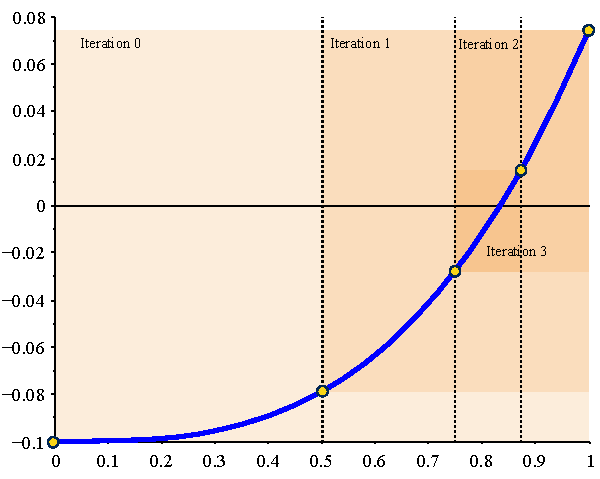
\includegraphics[scale=1]{./pics/f1_tol.pdf}
% \end{center}
% \caption{ \label{fig:fn:tol}
%  Illustration of $x$- and $y$-tolerances for bisection iterations}
%\end{figure}
%
%\newpage
%
%It takes very little text to fill a page in this format, but there is even less text on most of these sample pages.
%
%\section{Why we are doing it}
%It is usually a good idea to give reasons for your research.  If you do not, the people who payed you to waist all that time will feel really bad about it, and then they will not provide the same opportunity to future students.
%
%\newpage
%
%I need this page to see what even-numbered pages look like.
%
%\appendix
%\chapter{Methods}
%Here is how to implement the methods.
%
%\begin{program}
% \begin{verbatim}
%  (A map of the United States)
% \end{verbatim}
% \caption{Map of the United States}
%\end{program}
%
%\section{Bisection}
%The easiest method.
%
%\begin{equation}
%x_k = \frac{a_k+b_k}{2}
%\end{equation}
%
%\section{False Position}
%The next one.
%
%
%\chapter{Using Appendices}    \label{app:appendix}
%This appendix contains the portion of the users' manual that describes
%how to use appendices with this template.  It is put in this appendix
%rather than in Chapter \ref{chap:manual} simply so that there are two
%appendices, so that a list of appendices can appear earlier in the
%document.
%
%\section{Starting the Appendices}
%Actually, using appendices is quite simple.  Immediately after the end
%of the last chapter and before the start of the first appendix, simply
%enter the command \verb|\appendix|.  This will tell \LaTeX~to change
%how it interprets the commands \verb|\chapter|, \verb|\section|,
%\textit{etc.}
%
%Each appendix is actually a chapter, so once the \verb|\appendix|
%command has been called, start a new appendix by simply using the
%\verb|\chapter| command.
%\begin{code}
%\appendix
%\chapter{The First Appendix}
%...
%
%\chapter{The Boring Part That Is Not in the Chapters}
%\end{code}
%
%Note that the \verb|\appendix| command should be called only
%once--not before the start of each appendix.
%
%\section{Lists Including the Appendices}
%As mentioned in Section \ref{ssec:lists}, the command
%\begin{code}
%\showlistofappendices
%\end{code}
%must appear in the preamble if there are more than one appendices.  For
%some reason, Rackham does not want the individual appendices and their
%sections to appear in the Table of Contents, so a special List of
%Appendices page (which must occur in the Table of Contents!) is required
%as a sort of extension to the Table of Contents.
%
%This does not require a user of this template to do anything, but it is
%so silly that I felt it was worth explaining.  Also, there is nowhere
%for the sections or subsections of appendices to show up in the Table of
%Contents or any of the lists, but they do still create navigation tabs
%in a modern PDF viewer.
%
%
%
%% Using AIAA bibliography style since I'm in aero.
%\bibliographystyle{aiaa}
%% Give this command the relative path to the .bib file.
%\bibliography{./tex/thesis-bib}

\end{document}
